%%%%%%%%%%%%%%%%%%%%%%%%%%%%%%%%%%%%%%%%%%%%%%%%%%%
%% LaTeX book template                           %%
%% Author:  Amber Jain (http://amberj.devio.us/) %%
%% License: ISC license                          %%
%%%%%%%%%%%%%%%%%%%%%%%%%%%%%%%%%%%%%%%%%%%%%%%%%%%

\documentclass[a4paper,11pt,usenames,dvipsnames]{book}
\usepackage[T1]{fontenc}
\usepackage[utf8]{inputenc}
\usepackage{lmodern}
%%%%%%%%%%%%%%%%%%%%%%%%%%%%%%%%%%%%%%%%%%%%%%%%%%%%%%%%%
% Source: http://en.wikibooks.org/wiki/LaTeX/Hyperlinks %
%%%%%%%%%%%%%%%%%%%%%%%%%%%%%%%%%%%%%%%%%%%%%%%%%%%%%%%%%
\usepackage{hyperref}
\hypersetup{
    colorlinks,
    linktoc=all,
    citecolor=blue,
    filecolor=blue,
    linkcolor=blue,
    urlcolor=blue
}
\usepackage{color}
\usepackage{graphicx}
\usepackage[english]{babel}
\usepackage{tcolorbox}

\usepackage{fancyvrb} % To draw boxes around some verbatim text

\usepackage[margin=1in]{geometry} % To increase margin width

\usepackage{sectsty}
\chapterfont{\color{MidnightBlue}}
\sectionfont{\color{MidnightBlue}}
\subsectionfont{\color{MidnightBlue}}
\subsubsectionfont{\color{MidnightBlue}}
%%%%%%%%%%%%%%%%%%%%%%%%%%%%%%%%%%%%%%%%%%%%%%%%%%%
% First page of book which contains 'stuff' like: %
%  - Book title, subtitle                         %
%  - Book author name                             %
%%%%%%%%%%%%%%%%%%%%%%%%%%%%%%%%%%%%%%%%%%%%%%%%%%%

% Book's title and subtitle
\title{\Huge \textbf{PALEOSTRIP v1.0}  \\ \huge  User Manual}
% Author
\author{\textsc{Florence Colleoni....others}\thanks{\url{fcolleoni@inogs.it}}}


\begin{document}

\frontmatter
\maketitle


%%%%%%%%%%%%%%%%%%%%%%%%%%%%%%%%%%%%%%%%%%%%%%%%%%%%%%%%%%%%%%%%%%%%%%%%
% Auto-generated table of contents, list of figures and list of tables %
%%%%%%%%%%%%%%%%%%%%%%%%%%%%%%%%%%%%%%%%%%%%%%%%%%%%%%%%%%%%%%%%%%%%%%%%
\tableofcontents

\mainmatter

%-----------------------------------------------------------
% BEFORE STARTING
%-----------------------------------------------------------
\chapter{Before starting}

\section{Acknowledgements}\label{sec:acknowledgement}

PALEOSTRIP has been funded by several national Italian programs:
\begin{itemize}
\item PNRA18\_00002, ``Onset of Antarctic Ice Sheet Vulnerability to Oceanic conditions (ANTIPODE)'' 
\item PNRA16\_00016, ``West Antarctic Ice Sheet History from Slope Processes–Eastern Ross Sea (WHISPERS)'' 
\item MAECI bilateral Italy-US project US16GR04, ``Global Sea Level rise \& Antarctic Ice Sheet Stability predictions: guessing future by learning from past(GLSAISS)''.
\end{itemize}


\section{License}\label{sec:license}

PALEOSTRIP is distributed under the \href{https://www.gnu.org/licenses/gpl-3.0.html}{GNU General Public License v3.0}:\\\\

%\begin{tcolorbox}[colback=lightgray]
\begin{Verbatim}[frame=single]
Copyright (C) 2021 PALEOSTRIP Authors
This file is part of PALEOSTRIP.

PALEOSTRIP is free software; you can redistribute it and/or modify it under 
the terms of the GNU General Public License as published by the Free 
Software Foundation; either version 3 of the License, or (at your option) 
any later version.

PALEOSTRIP is distributed in the hope that it will be useful, but WITHOUT ANY
WARRANTY; without even the implied warranty of MERCHANTABILITY or FITNESS
FOR A PARTICULAR PURPOSE.  See the GNU General Public License for 
more details.

You should have received a copy of the GNU General Public License
along with PALEOSTRIP; if not, write to the Free Software
Foundation, Inc., 51 Franklin St, Fifth Floor, Boston, MA  02110-1301  USA.
\end{Verbatim}
%\end{tcolorbox}

\section{PALEOSTRIP design philosophy}\label{sec:design}

PALEOSTRIP is an open-source \texttt{MATLAB} code easy to use thanks to its Graphic User Interface. The structure of the software is transparent and flow a logical flow. The code is developed so that any modification to the source can be easily incorporated and new parameterisations can be easily implemented with a ''plug-and-play`` philosophy.\\

\noindent PALEOSTRIP has been designed so that the user can separate the effect of the various corrections needed and thus all corrections can be switch on or off from the GUI.\\


\section{PALEOSTRIP: what it does and does not do}\label{sec:design}

PALEOSTRIP is a software to perform backtracking, i.e., retrieve paleo-water depths from a computed subsidence history. It does not allow to carry out backstripping, i.e., retrieve the subsidence history from input paleo-water depths. Backstripping will be considered for a future release of PALEOSTRIP.




%-----------------------------------------------------------
% GETTING STARTED
%-----------------------------------------------------------
\chapter{Getting started}

The aim of this User Manual is not to describe the physics embedded within the code. Most of the physics embedded in PALEOSTRIP is based on \textcolor{red}{Allen and Allen, 2nd, 1993} and is described in \textcolor{red}{Colleoni et al., submitted to GMD - link to GMD Discussion}.  In the following, we detail the options available from PALEOSTRIP GUI and explain how to run PALEOSTRIP built-in examples. 


\section{Requirements}\label{sec:requirements}

 \textbf{MATLAB v2019 or later versions}: \\PALEOSTRIP has been developed using \textbf{\texttt{MATLAB v2019b}}. More specifically, the Graphical User Interface is coded with the App Designer toolbox that will substitute the previous toolbox \texttt{GUIDE} from MATLAB v2020 onward. Thus it is important compiling and running PALEOSTRIP using \textbf{\texttt{MATLAB v2019} or later versions}. In addition, the MATLAB version must include the App Designer Toolbox otherwise, it will be impossible to launch the Graphical User interface.\\
 
  \noindent  \textbf{The Graphical User Interface}:\\ PALEOSTRIP cannot not run without its GUI. However, the source code could be modified to do so without requiring too much extra work. In practice, the user would need to create a routine to open data files and set physical options to be passed to the main routine of PALEOSTRIP (\texttt{backtracking.m}).\\

 

\section{Download \& Install}\label{sec:installing}
\subsection{Get PALEOSTRIP}

PALEOSTRIP is hosted on GitHub and can be downloaded here:\\
\textcolor{red}{\href{}{PALEOSTRIP v1.0}}

\subsection{PALEOSTRIP directories}

PALEOSTRIP comes with the GUI source code, some accessory files and two directories:

\begin{itemize}
\item \texttt{PALEOSTRIP\_App.mlapp}: source code of the GUI to be opened with the App Designer toolbox (just double click on it).
\item \texttt{COPYING}: terms of the GNU GPL v3.0 license.
\item \texttt{OGS\_transparent.png}:  logo of the main hosting research institution.
\item \texttt{doc/}: present User Manual.
\item \texttt{auxiliary/}: all the source code of the routines called by the GUI.\\
\end{itemize}


\textbf{It is important that all the listed files and directories above are located in the same directory.}\\


The \texttt{auxiliary/} directory contains all the routines called by the GUI and is subdivided as follows:
\begin{itemize}
\item \texttt{backtracking.m}: \\ Main routine of PALEOSTRIP called by the GUI.This routines performs the sediment decompaction and subsidence and sea level corrections.  It calls \texttt{thermal\_subsidence.m}, \texttt{isostasy.m} and \texttt{dynamic\_topography.m}. 
\item \texttt{dynamic\_topography.m}: \\reads user-based GUI dynamic topography correction.
\item \texttt{isostasy.m}: \\ Calculates isostatic compensation for sediment removal (2D/3D flexure or Airy).
\item \texttt{sealevel.m}: \\ Calculates sea level change correction based on the water loading changes relative to present-day (using flexure or Airy isostasy). \textbf{This correction cannot be computed if isostasy is switched off}.
\item \texttt{thermal\_subsidence.m}: \\ provides the time-evolving syn-rift and post-rift thermal subsidence correction based on the 1D model of \textcolor{red}{McKenzie et al. (1978)}.
\item \texttt{isostasy/}: \\ contains the routines for 3D and 2D flexural isostasy \textcolor{red}{(Cardozo et al.)}.
\item \texttt{mesh\_grid/}: \\ routines to regrid 3D variables (lithospheric elastic thickness and sediment layers) to expand the original grid domain for flexural isostasy purpose or for plotting results.
\item \texttt{plot\_save/}: routines to plot backtracked variables and save results to ASCII files. Also contains routines to extract and save 2D sections or 1D well from backtracked data (See GUI description).
\item \texttt{read\_data/}: \\ various routines to read input data provided through the GUI.
\end{itemize} 

\newpage
\subsection{Run PALEOSTRIP}

To run PALEOSTRIP:
\begin{itemize}
\item [\textbf{1}] Open Matlab and browse the directories to load PALEOSTRIP directory
\item [\textbf{2}] Double click on the \texttt{PALEOSTRIP\_App.mlapp} GUI source code. This will open the \texttt{App Designer toolbox}.
\item [\textbf{3}] Click on the green arrow on the top menu to execute the code, it opens the GUI (Figure~\ref{appdesign}). It is thus important to retrieve a \texttt{Matlab v2019b }version or later, including the \texttt{App Designer toolbox}.\\
\end{itemize}

\begin{figure}[!h]
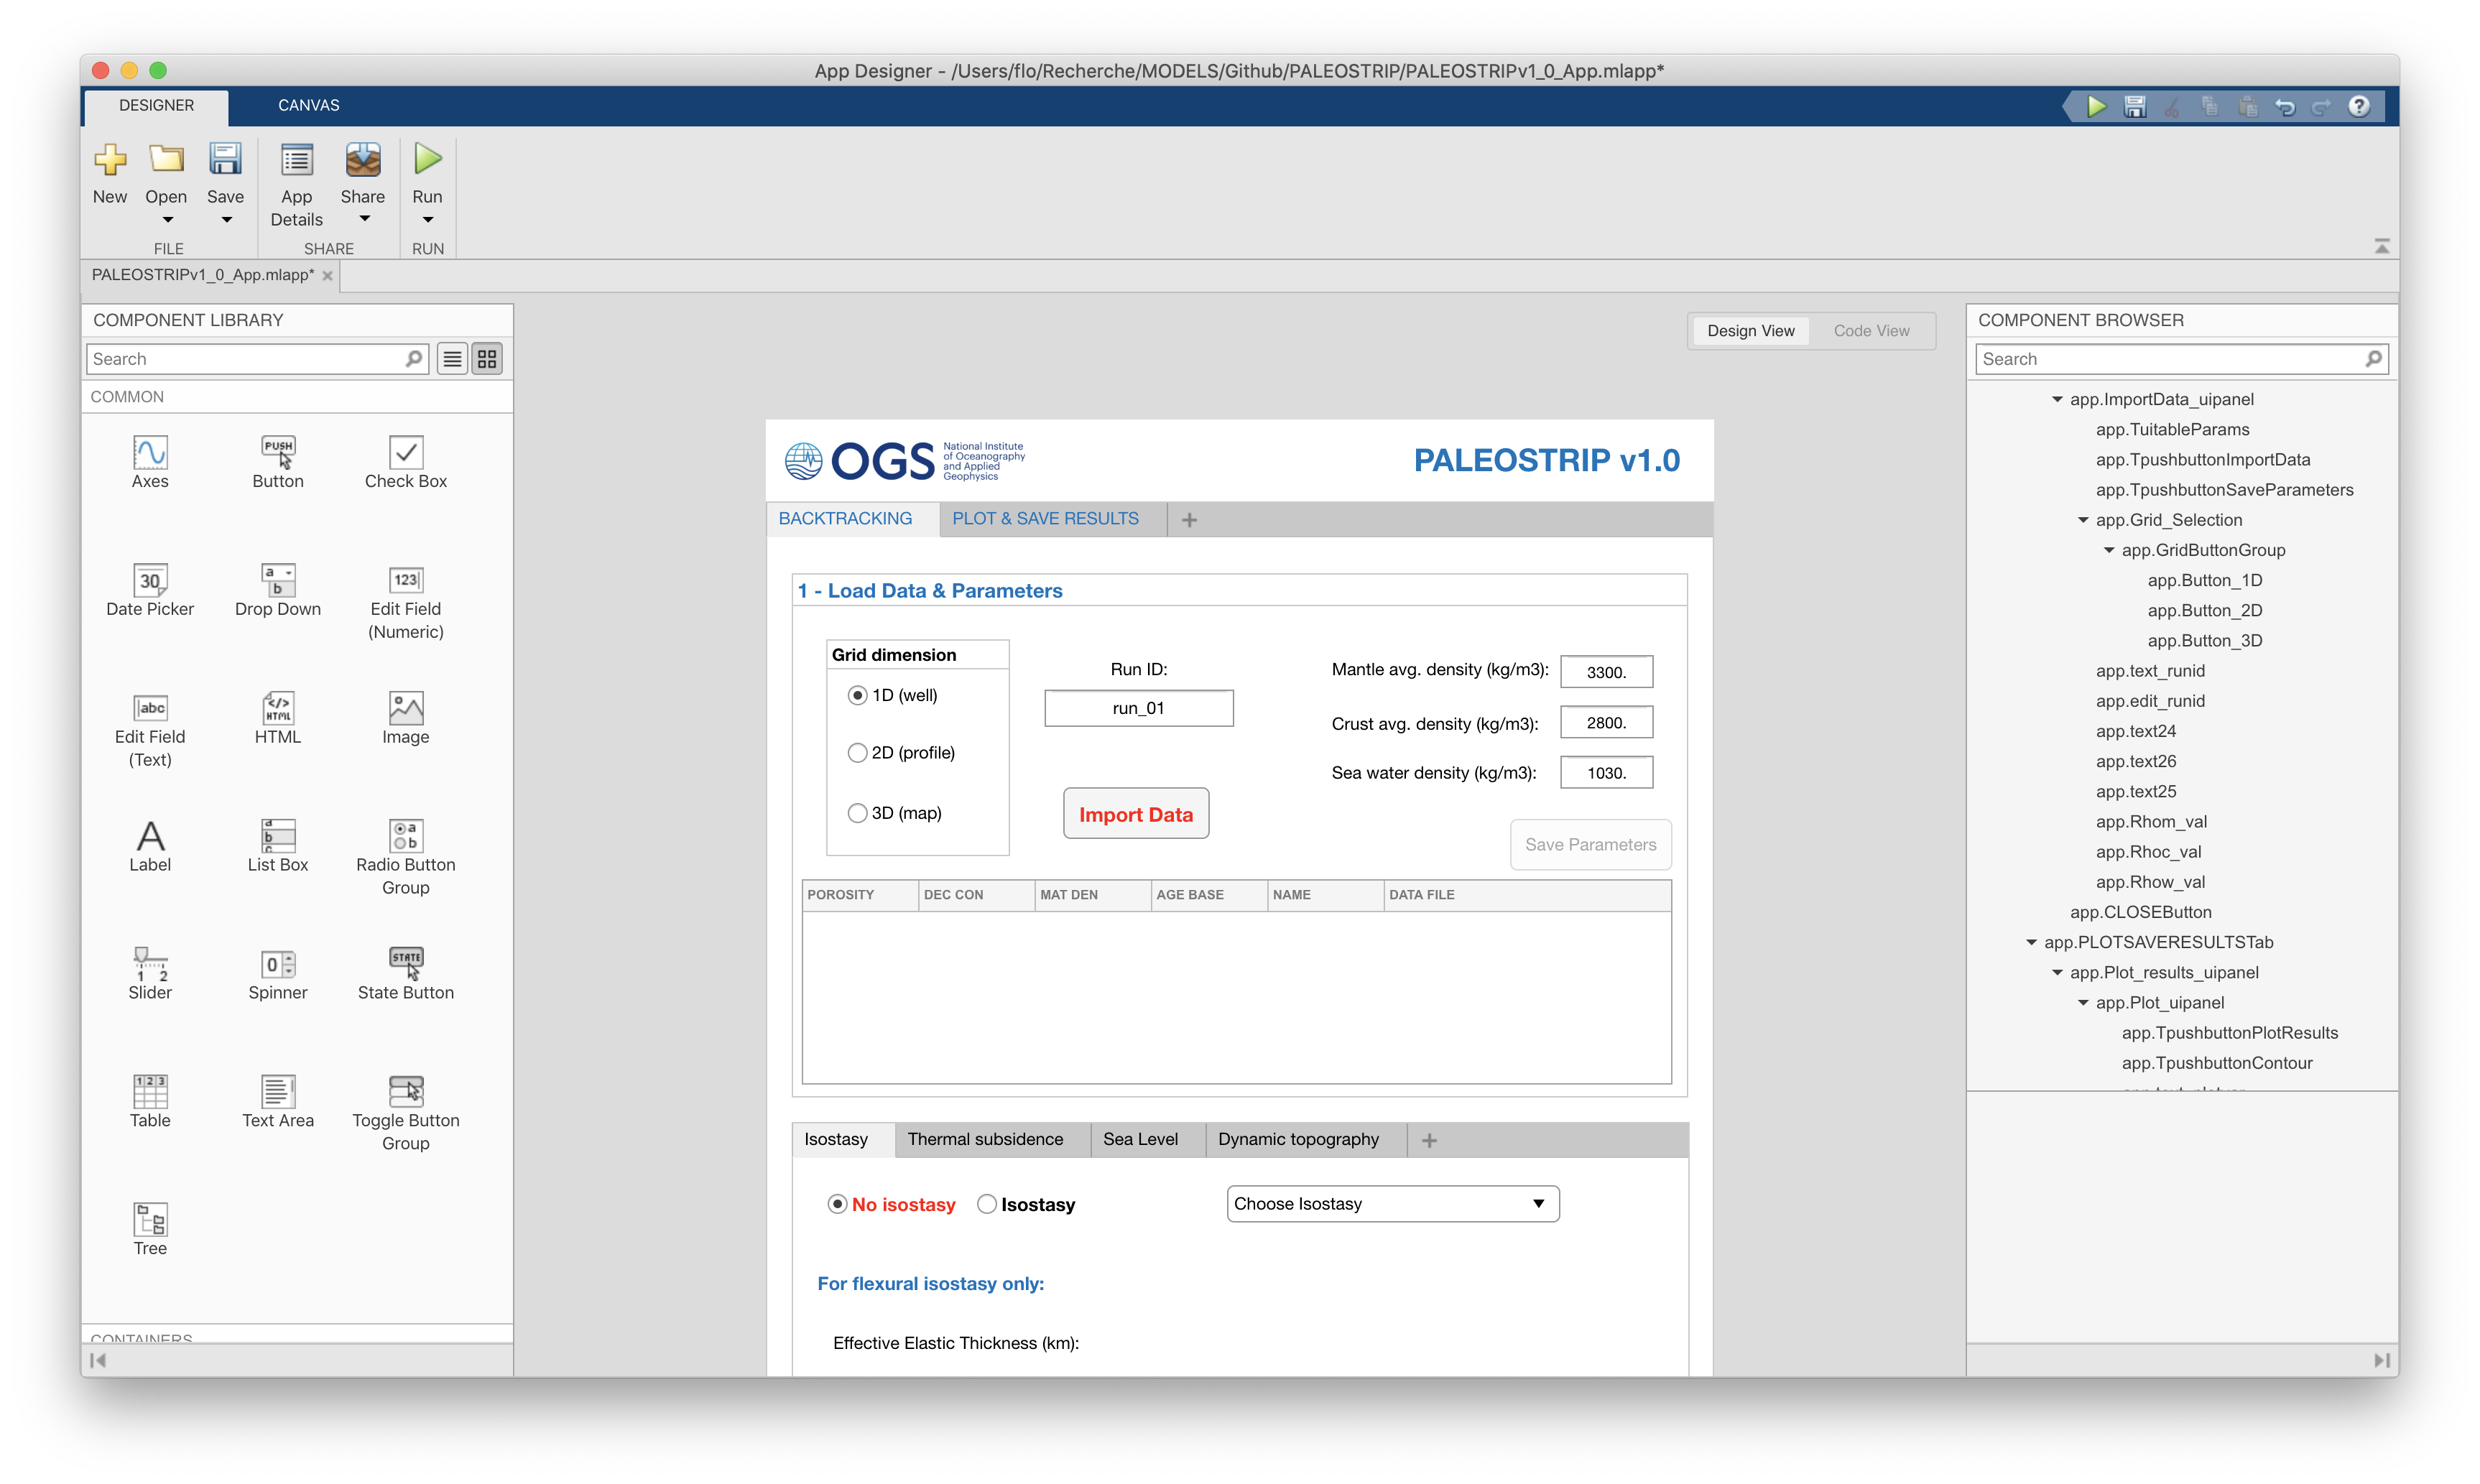
\includegraphics[width=\linewidth]{Figures/Fig_00_App_designer_MATLAB.png}
\caption{App Designer interface. Click on ''Run`` (green arrow) on top menu to launch the GUI.}
\label{appdesign}
\end{figure}


\subsubsection*{PALEOSTRIP as a stand-alone application:}
To avoid using MATLAB systematically, PALEOSTRIP can be exported with its MATLAB libraries as a stand-alone application from the App Designer Toolbox (''Share`` button on top menu in Figure~\ref{appdesign}). After exportation, the user will not need to use MATLAB anymore.\\\\
Exporting Stand-alone application is not cross-plateforms. For example, to export PALEOSTRIP as stand-alone for Linux will require MATLAB LINUX libraries to be wrapped-up within the package.\\

\noindent More about packaging stand-alone applications:\\
\href{https://it.mathworks.com/help/matlab/creating_guis/package-apps-in-app-designer.html}{https://it.mathworks.com/help/matlab/creating\_guis/package-apps-in-app-designer.html}


\newpage
\section{PALEOSTRIP GUI options}\label{sec:options}

The GUI is subdivided in two main tabs: (1) a tab to import data, choose physical options and run backtracking; (2) a tab to plot, extract and save results (Figure~\ref{gui}).

\begin{figure}[!h]
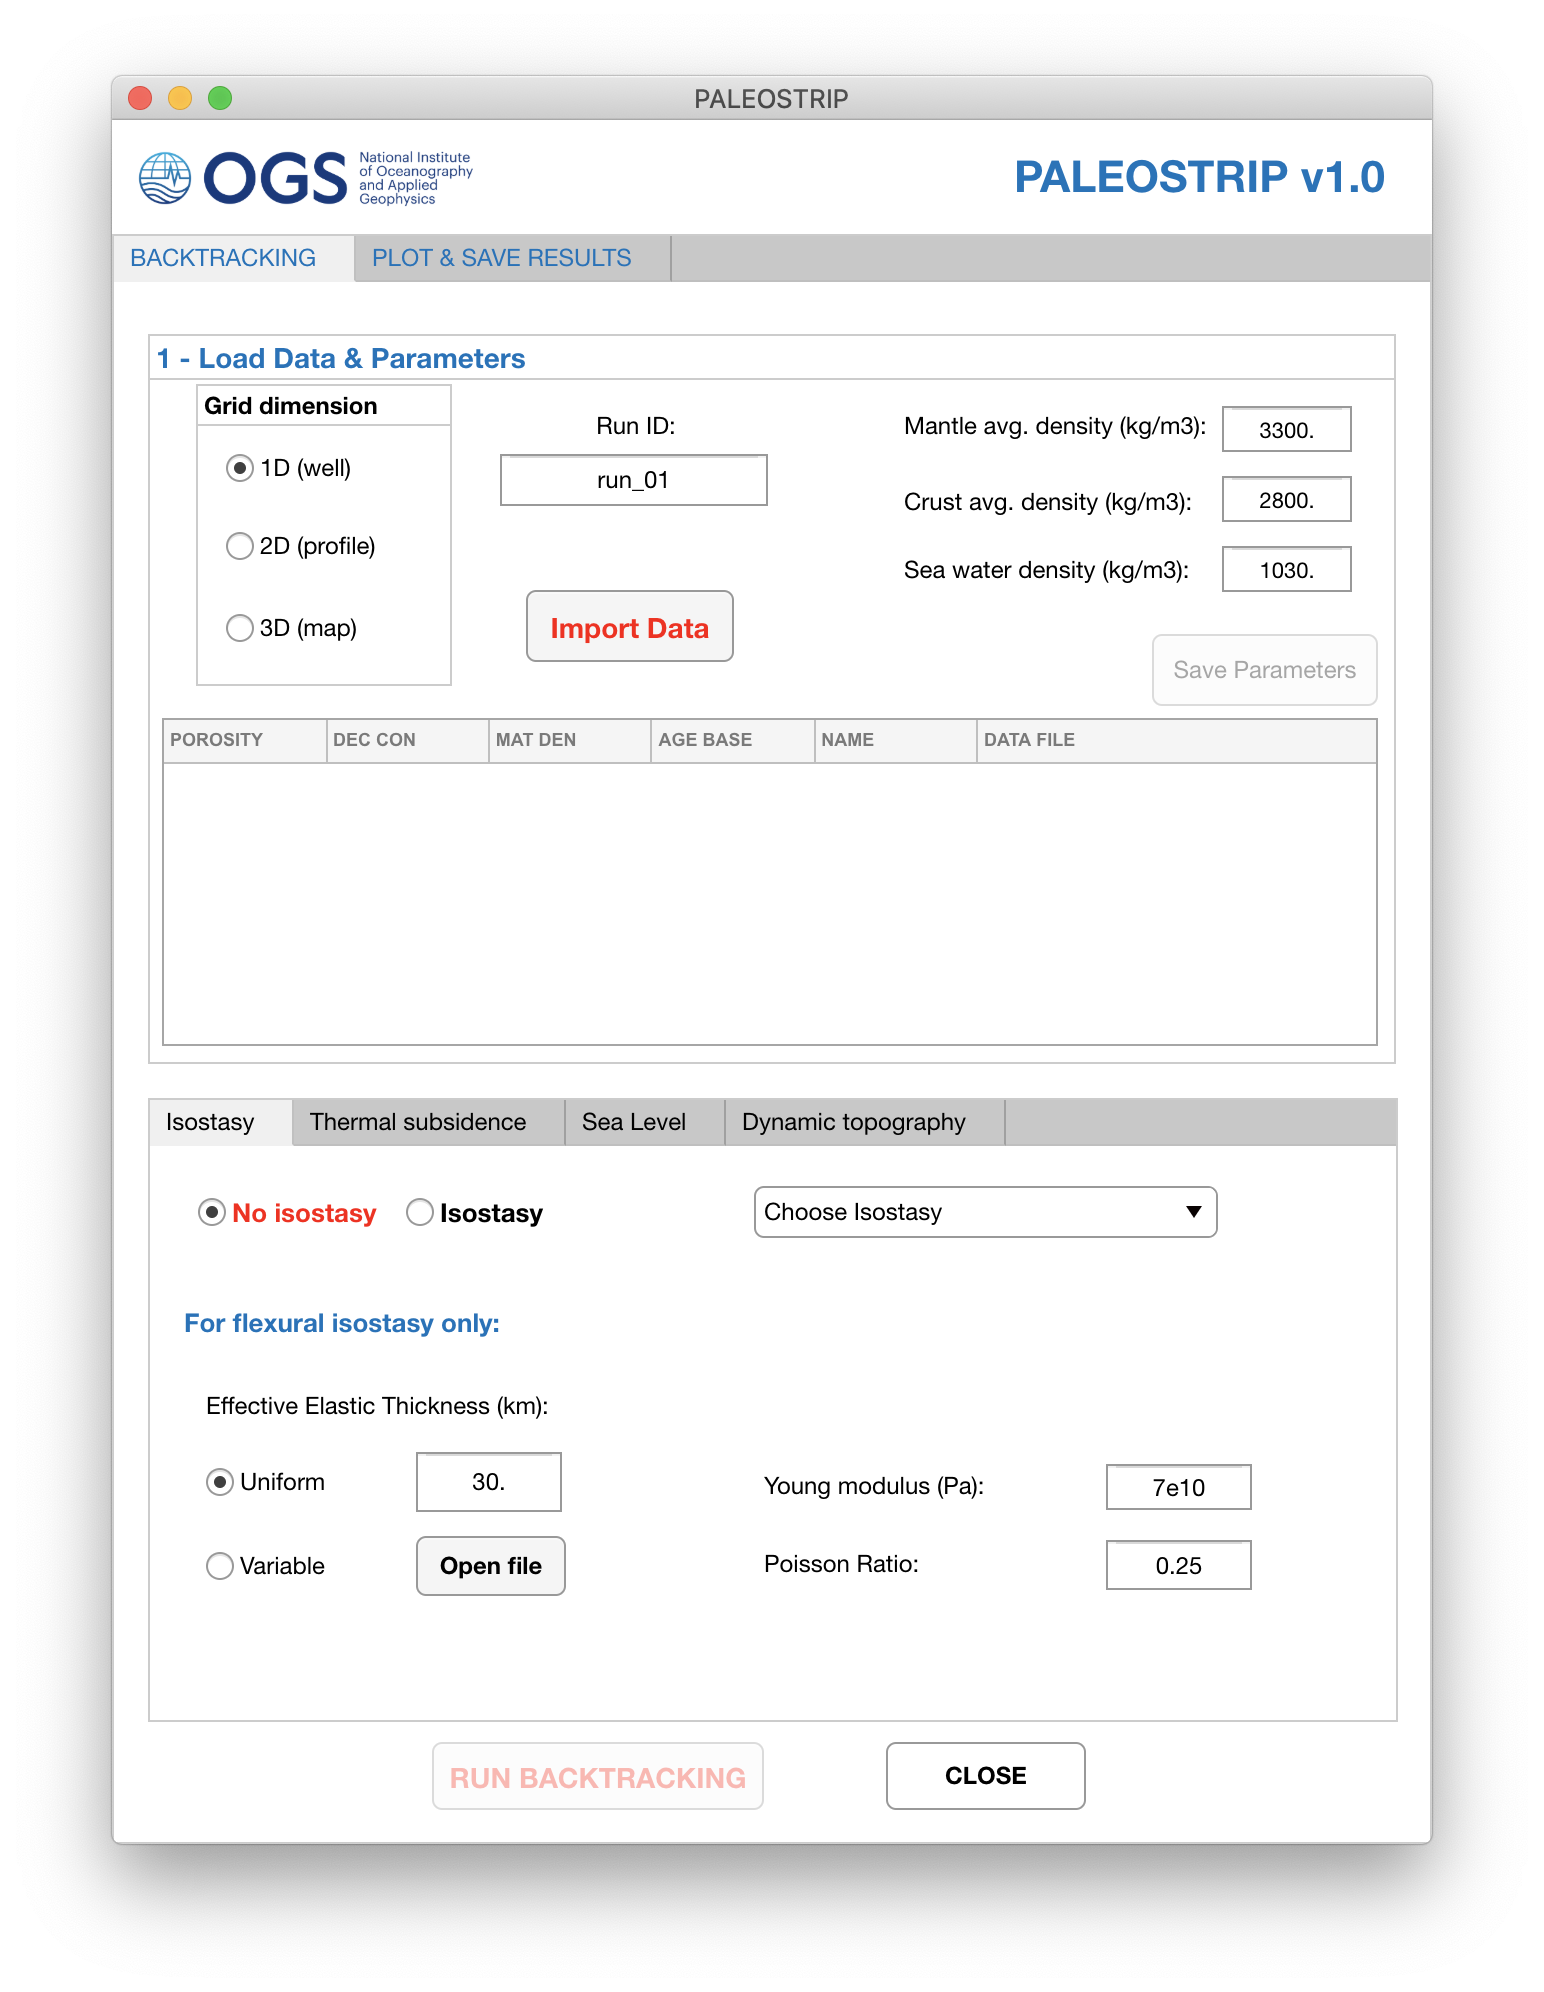
\includegraphics[width=\linewidth]{Figures/Fig_01_PALEOSTRIP_GUI.png}
\caption{PALEOSTRIP GUI}
\label{gui}
\end{figure}

\noindent Almost any physical parameter and constant included in the various routines can be modified from the GUI. This is at the base of PALEOSTRIP.

\subsection{Import data}

The upper part of the GUI is dedicated to import the user input data files and set grid dimensions. 

\subsubsection*{Data grid dimension:}
It is important for PALEOSTRIP to know in advance the type of data that will be considered for calculation, i.e. if the user is decompacting a well, a vertical section or horizontal maps. Grid dimension must be indicated to PALEOSTRIP that will check the format of the input files:\\
\begin{itemize}
\item 1D (well): input data contain only one column.
\item 2D (section): input data contain two columns.
\item 3D (maps): input data contain three columns.
\end{itemize}

\noindent Grid dimension is passed along to the other routines of PALEOSTRIP for backstracking calculations. It is thus important to indicate this option. \\

\subsubsection*{Import Data:}
\noindent Clicking on \textbf{\color{red}{Import Data}} opens a diaologue from which the user can browse through directories and load input data files. 
\begin{tcolorbox}[colback=GreenYellow]
It is important that all the data files (horizon\_depth.dat) and lithological parameters (litho.par) are located in the \textbf{same directory}.\\\\
The input directory must contain only the needed files, i.e., \textbf{one} lithological parameters file \texttt{litho.par} and the corresponding \textbf{N} files \texttt{horizon\_depth.dat} (the number of files \textbf{N} is indicated within \texttt{litho.par}. Note that the input directory can contain other sub-directories.
\end{tcolorbox}

\noindent Once loaded and if the format of the files is correct, the GUI will display the lithological parameters from the *.par input file within the Table located in the center of the GUI. \\

\noindent See Section~\ref{format} about files format and Section~\ref{examples} about running examples for more indications on how to provide input data to PALEOSTRIP.\\



\subsubsection*{Physical constants:}
\noindent The user can modify the values of constants for Mantle, Crust and Seawater density. Default values are pre-indicated on the GUI and will be used if not otherwise modified by the user.\\

\subsubsection*{Simulation string name:}
\noindent Finally, the user can provide the name of the backtracking simulation to be run. Default set-up name is ''run\_01'' but there is basically no restrictions on the length of the string. \\

\noindent This string will be automatically concatenated to output files if the user will choose to save the results. \textit{The string can be modified anytime before saving outputs} (See section~\ref{save}).

%-----------ISOSTASY-------------------
\newpage
\subsection{Isostasy}
In the bottom part of the GUI, four tabs allow to select the physical parameters related to the various corrections needed to backtrack sediments. Two methods of isostasy have been implemented:
\begin{itemize}
\item The Airy local isostasy (1D, 2D, 3D grids)
\item Flexural isostasy (2D and 3D grids)
\end{itemize}

\noindent By default, isostasy is switched off through the button \textcolor{red}{\textbf{No isostasy}}. To switch it on the user must select "Isostasy" on the GUI.\\

\subsubsection*{Airy local isostasy}
Airy local isostasy can be selected from the drop menu in the Isostasy tab (Figure~\ref{gui}). No other options need to be set or selected for this method.\\

\noindent The Airy local method can be used for 1D, 2D or 3D grids.

\subsubsection*{Flexural isostasy}
Flexural isostasy can be selected from the drop menu (Figure~\ref{gui}). Along with this method, the user may set all the other options from this tab. PALEOSTRIP uses the default values indicated in the GUI if not modified by the user:\\

\noindent \textbf{Lithospheric Elastic Thickness:}\\ 
PALEOSTRIP allows flexural isostasy with spatially uniform or spatially variable elastic thickness. Variable elastic thickness requires an input file (user-based) containing the spatially variable values of lithospheric elastic thickness.

\begin{itemize}
\item \underline{Uniform elastic thickness}: select ''\texttt{Uniform}'' and insert a value (in km) in the nearby field.\\ 
\item \underline{Variable elastic thickness}: select "\texttt{Variable}" from the GUI and click on \textbf{Open file}. This will open a dialogue from which to browse in directories and access 2D or 3D elastic thickness user-provided file.  \textbf{\textcolor{red}{Note that the input file must contain values provided on the same grid (horizontal resolution and projection) as input sediment data}}. PALEOSTRIP does not provide any ways to interpolate data on a chosen grid. See Chapter~\ref{preproc} about pre-processing data.
\end{itemize}

\noindent Other options:
\begin{itemize}
\item \underline{Physical constants}: Young Modulus and Poisson ratio can be set from the GUI. Default values will be used if not modified.
\end{itemize}


%---------THERMAL SUBSIDENCE
\newpage
\subsection{Thermal Subsidence}
PALEOSTRIP adopts the 1D-thermal subsidence model from McKenzie (1978) that assumes an instantaneous stretching (syn-rift) and a unique rifting phase. As for isostasy, the option is deactivated (\textcolor{red}{\textbf{No thermal subs.}} is selected by default) and the user must select "\textbf{Thermal subsidence}" on the GUI to activate it. In the tab, several values have to be provided by the user (Figure~\ref{TS_gui}):\\

\begin{figure}[!h]
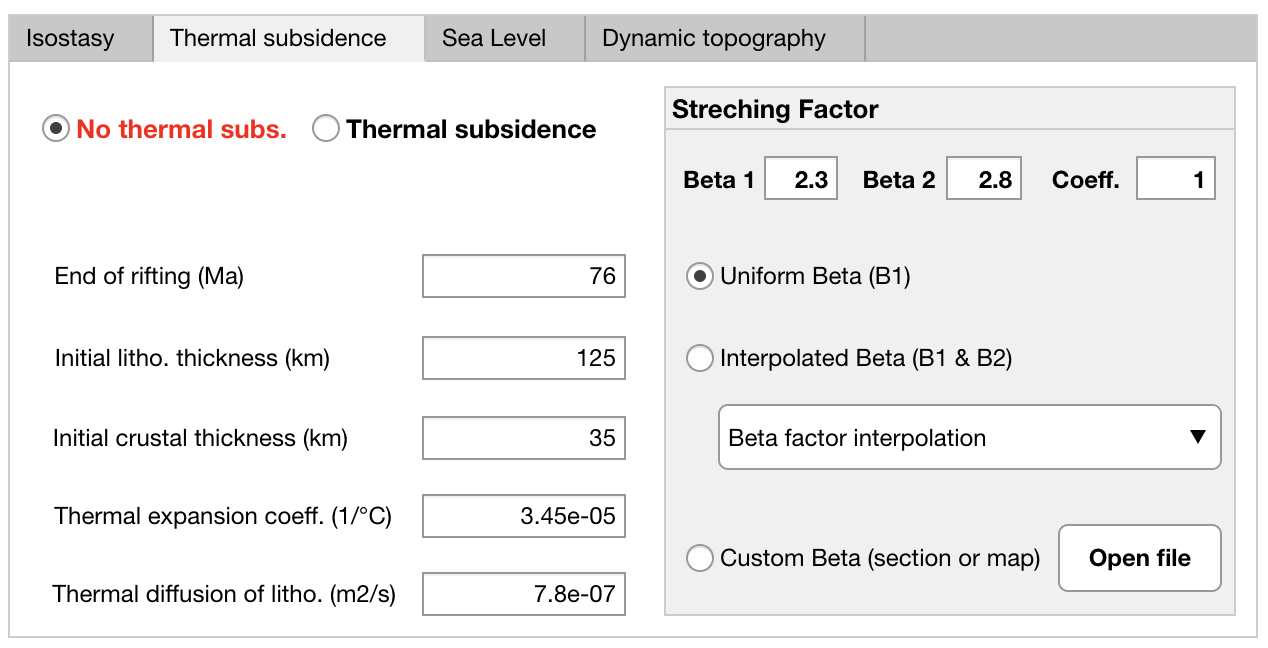
\includegraphics[width=\linewidth]{Figures/Fig_02_Thermal_subsidence.png}
\caption{PALEOSTRIP GUI - Thermal subsidence tab.}
\label{TS_gui}
\end{figure}

\begin{itemize}
\item \underline{End of rifting (Ma)}: corresponds to the age of the end of the rifting phase and must be provide in Million years ago. For example, if a rifting ends at 14 Ma, the user should set the value to "14". Note that the age must be \textbf{positive} even if it refers to the past. This value is considered as the starting point of the post-rift subsidence calculation.

\item \underline{Initial litho. thickness (km)}: corresponds to the lithospheric thickness at the beginning of the rifting phase. In literature, 125 km is considered as a standard value, but we strongly recommend to the user to check because this parameter impacts substantially on the amount of thermal subsidence coomputed.

\item \underline{Initial crustal thickness (km)}: which differs from "\textit{Initial litho. thickness}" option, corresponds to the crustal thickness at the beginning of the rifting phase. As for the "\textit{Initial litho. thickness}" option, the crustal thickness impacts notably on the amount of thermal subsidence computed.

\item \underline{Thermal expansion coeff. (1/$\deg$C)}: is the thermal expansion coefficient of the asthenosphere and is set to a standard literature value. But we provide the opportunity to the user to modify it to account for different geodynamic contexts.

\item \underline{Thermal diffusion of litho. (m2/s)}: is the thermal diffusion of the lithosphere and is set to a standard literature value. But we provide the opportunity to the user to modify it to account for different geodynamic contexts.
\end{itemize}

\begin{tcolorbox}[colback=GreenYellow]
Note that PALEOSTRIP does not allow to provide spatially variable lithospheric and crustal thickness. This will be the object of a PALEOSTRIP future release.
\end{tcolorbox}

\subsubsection*{Stretching factor}

\noindent The second half of the tab is dedicated to the stretching factor (or Beta factor $\beta$). It can be set in three different ways:

\begin{itemize}
\item \underline{Uniform Beta}: this option considers the spatially uniform value provided in \texttt{Beta1} field on the GUI. In this case, the beta factor is identical over the entire section/domain.

\item \underline{Interpolated Beta}: this options considers the values provided in \texttt{Beta1} and \texttt{Beta2} fields on the GUI. Two different interpolation methods are then available from the drop menu "\texttt{Beta factor interpolation}": \\ 
(1) \texttt{Linear interpolation} interpolates along X direction between \texttt{Beta1} and \texttt{Beta2} from the left to the right of the section or the domain (rightmost side will tend to \texttt{Beta2} and leftmost points will tend to \texttt{Beta1}); \\

(2) \texttt{Step-Wise interpolation} applies uniformly \texttt{Beta1} left of a X limit and \texttt{Beta2} right of this value. The X limit is determined by means of a coefficient prescribed on the GUI \texttt{coeff}. This coefficient varies between 0 and 1. For example: if \texttt{coeff} is set to 0.4, then X limit will be set to $Xmin+(Xmax - Xmin)*0.4$, where $Xmin$ and $Xmax$ are the min and max X coordinates of the section/domain.
 
\end{itemize}




%---------- SEA LEVEL ---------------
\newpage
\subsection{Sea Level correction}
Backtracking sediments implies to reconstruct the paleo-water depth at a given time which is obviously influenced by eustatic sea level changes (and also regional ones). As for \texttt{Isostasy} and \texttt{Thermal subsidence}, Sea level correction is deactivated by default and need to be switch on by selecting \texttt{Sea Level changes} on the GUI. PALEOSTRIP allows sea level to be corrected in three different ways (Figure~\ref{sea_level_gui}):

\begin{itemize}
\item \underline{Uniform sea level change (m)}: sets spatially uniform and constant in time sea level correction \textbf{in meters}. Default value is 0 m if not set otherwise by the user.

\item \underline{1D timeseries}: uses \textcolor{red}{Haq et al.} or \textcolor{red}{Miller et al. (2020)} and linearly interpolates sea level values (in meters) at the ages of each sediment horizon indicated in the \texttt{litho.par} file.

\item \underline{User-based Sea Level:} allows to provide a 1D timeseries of sea level changes (\texttt{1D timeseries}) or a spatially varying, but constant in time map of sea level changes (\texttt{2D map}) in meters, by clicking on \texttt{Open file}. In the case of \textbf{2D maps}, sea level values must be provided \textbf{on the same grid than for horizon\_depth.dat input files}. Providing 2D maps is of interest for polar regions where sea level changes are not eustatic but are affected by the gravitational changes induced by ice sheet growth and decay and water loading.
\end{itemize}

\begin{tcolorbox}[colback=GreenYellow]
Note that PALEOSTRIP does not allow to provide a series of time-evolving 2D maps, but only allow one map of constant and spatially variable sea level changes to be used as input. This modification will be the object of a PALEOSTRIP future release.
\end{tcolorbox}

\begin{figure}[!h]
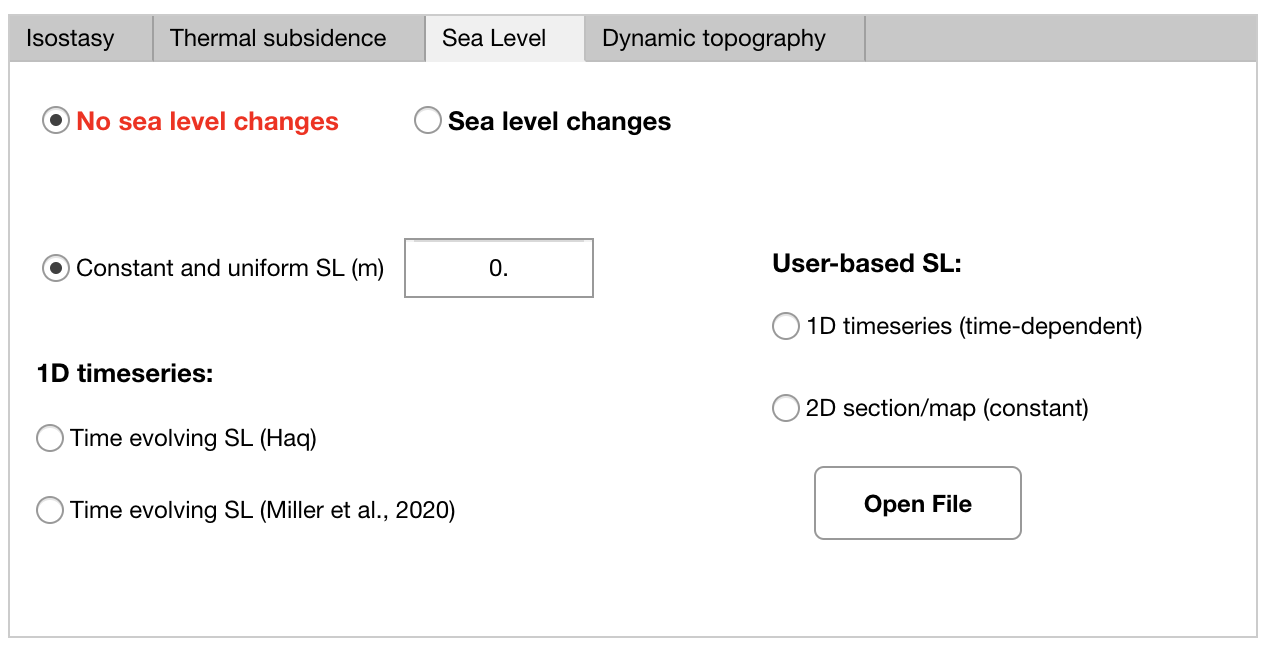
\includegraphics[width=\linewidth]{Figures/Fig_03_Sea_Level.png}
\caption{PALEOSTRIP GUI - Sea Level tab.}
\label{sea_level_gui}
\end{figure}


%---------- DYNAMIC TOPOGRAPHY
\newpage
\subsection{Dynamic topography}
The last tab is dedicated to dynamic topography correction (Figure~\ref{dyntopo_gui}). As for \texttt{Isostasy}, \texttt{Thermal subsidence} and \texttt{Sea level correction}, \texttt{Dynamic topography} is switched off by default and needs to be switch on by selecting \texttt{Dynamic topo.} on the GUI. Dynamic topography is corrected relatively to its present-day value. PALEOSTRIP provides two ways to account for this effect:

\begin{itemize}
\item \underline{Uniform correction (m)}: allows the user to set a spatially uniform and constant dynamic topography correction in meters \textbf{relative to present}.
\item \underline{1D timeseries (m)}: 
\item \underline{2D profiles/3D maps (m)}: allows the user to provide an ASCII files listing the names of a set of dynamic topography files (values in meters), indicating their corresponding age in Million years ago. For example: the time slices reconstructed by M\"uller et al., (2018): 

\begin{verbatim}
0,M1-0-Ma-Antar-spolar-kingdom.txt
10,M1-10-Ma-Antar-spolar-kingdom.txt
20,M1-20-Ma-Antar-spolar-kingdom.txt
30,M1-30-Ma-Antar-spolar-kingdom.txt
40,M1-40-Ma-Antar-spolar-kingdom.txt
50,M1-50-Ma-Antar-spolar-kingdom.txt
60,M1-60-Ma-Antar-spolar-kingdom.txt
70,M1-70-Ma-Antar-spolar-kingdom.txt
80,M1-80-Ma-Antar-spolar-kingdom.txt
90,M1-90-Ma-Antar-spolar-kingdom.txt
\end{verbatim}


The minimum number of dynamic topography files to be listed within the ASCII files is 2 (present-day and one paleo time slice). \\

PALEOSTRIP then linearly interpolates the dynamic topography to the ages of the input sediment horizons (\texttt{litho.par}). The correction is thus calculated relatively to present-day dynamic topography. 
\end{itemize}

\begin{tcolorbox}[colback=GreenYellow]
For 2D profiles/3D maps option:\\ 
- \texttt{First time slice} in the file list must necessary be \textbf{present-day dynamic topography} and \textbf{Age (Ma) must be set to 0}\\
- The other files must be provided in \textbf{chronological order, back in time}.\\
- All the files must be provided \textbf{on the same grid (horizontal resolution and geographical projection) as for input sediment files}.
\end{tcolorbox}


\begin{figure}[!h]
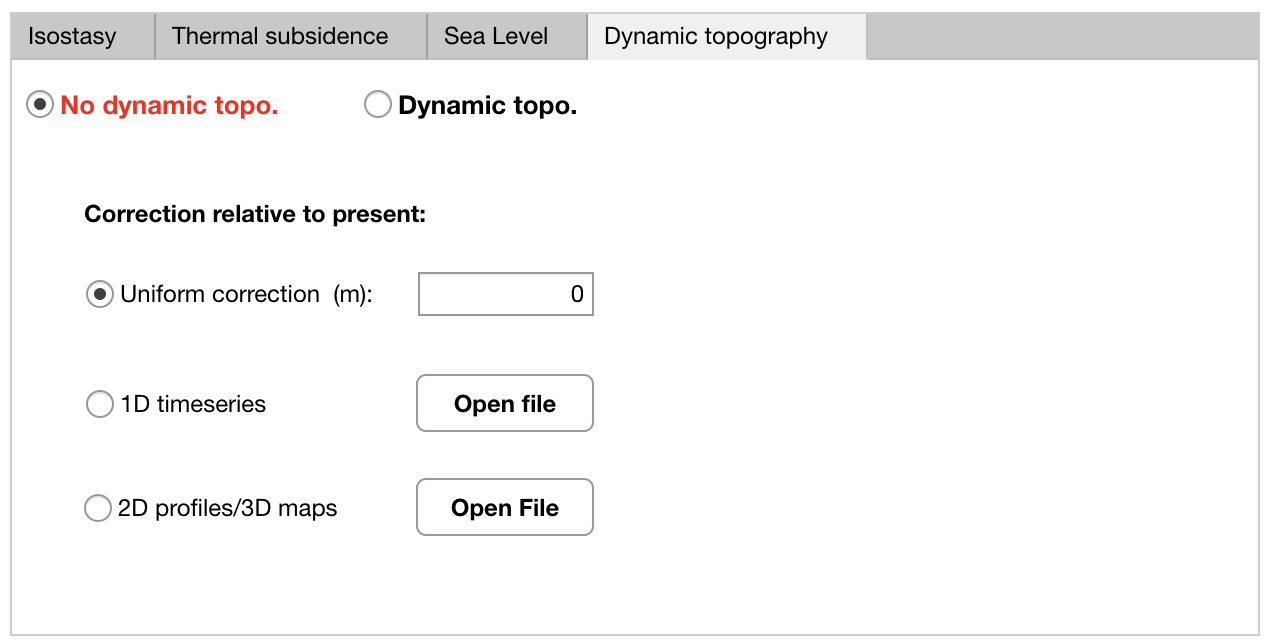
\includegraphics[width=\linewidth]{Figures/Fig_04_Dynamic_topography.png}
\caption{PALEOSTRIP GUI - Dynamic topography tab.}
\label{dyntopo_gui}
\end{figure}


%---------- LOG FILE
\newpage
\subsection{Log file}

To allow the user to remember the selected physical parameters and methods, PALEOSTRIP writes a log file. The log file contains all selected parameters and methods from the GUI. The file name uses the \texttt{String\_ID} character string from the GUI (Figure~\ref{gui}) and is named \texttt{backstracking\_log\_params\_String\_ID.txt}. The file is written in the PALEOSTRIP directory each time the user clicks on \textbf{\textcolor{red}{RUN BACKTRACKING}}. The file is overwritten if the \texttt{String\_ID} remains unchanged. Here is an example of log file:

\begin{verbatim}
------------------=------------------
=PALEOSTRIP PARAMETERS LOG= 
------------------=------------------
Grid dimension=2D
------------------=------------------
Astenosphere_density=3300.
Crustal density=2800.
Sea water density=1030.
------------------=------------------
Isostasy=Yes
Isostasy=Flexure (Green function)
Eff. Elastic Thick.=Uniform
Eff. Elastic Thick.=30
Young modulus=70000000000
Poisson Ratio=0.25
dx (spacing, km)=1
------------------=------------------
Sea Level=Yes
Sea Level=Miller
------------------=------------------
Thermal Subsidence=Yes
Age of rift (Ma)=76
Initial litho. thickness (km)=125
Initial crustal thickness (km)=35
Thermal diffusion coefficient (m2/s)=3.45e-05
Thermal expansion coeff. (1/C)=7.8e-07
Beta factor=Uniform
Beta factor 1=2.3
------------------=------------------
Dynamic Topography=No
------------------=------------------
=END OF LOG= 
------------------=------------------
\end{verbatim}


%------------RUNNING EXAMPLES-----------------------
\newpage
\section{Running examples}\label{examples}

Example files to test 1D, 2D and 3D backtracking are provided along with PALEOSTRIP on the GitHub repository: \texttt{examples.zip}.\\\\
\textbf{Input data repository can be located anywhere} and does not need to be (and preferably not) located within PALEOSTRIP main directory. Similarly as explained below, results can be saved in any directory out of the main PALEOSTRIP directory. \\

\noindent To set-up the various examples, just launch PALEOSTRIP GUI and import data from this examples directory for the selected case (1D, 2D or 3D). \\

\begin{tcolorbox}[colback=GreenYellow]
Note that it is important to select the "1D", "2D" and "3D" option on the GUI to inform PALEOSTRIP about the grid dimension to be passed along to the other sub-routines of the program.\\
\end{tcolorbox}

\noindent To run the selected case, just click on "\textcolor{red}{Run Backtracking}" at the bottom of the GUI once physical options have been chosen (Figure~\ref{gui}).\\

\noindent Appendix A visually documents each step of backtracking 3D maps.


%-------------- PLOT & SAVE OUPUTS
\newpage
\section{Plot outputs}\label{save}

PALEOSTRIP proposes basic plotting tools to visualize the outputs of the backtracking procedure as well as to save backtracked variables. The upper part of the  \texttt{PLOT \& SAVE RESULTS} tab is divided into two sections (Figure~\ref{plot_gui}). \\

\begin{figure}[!h]
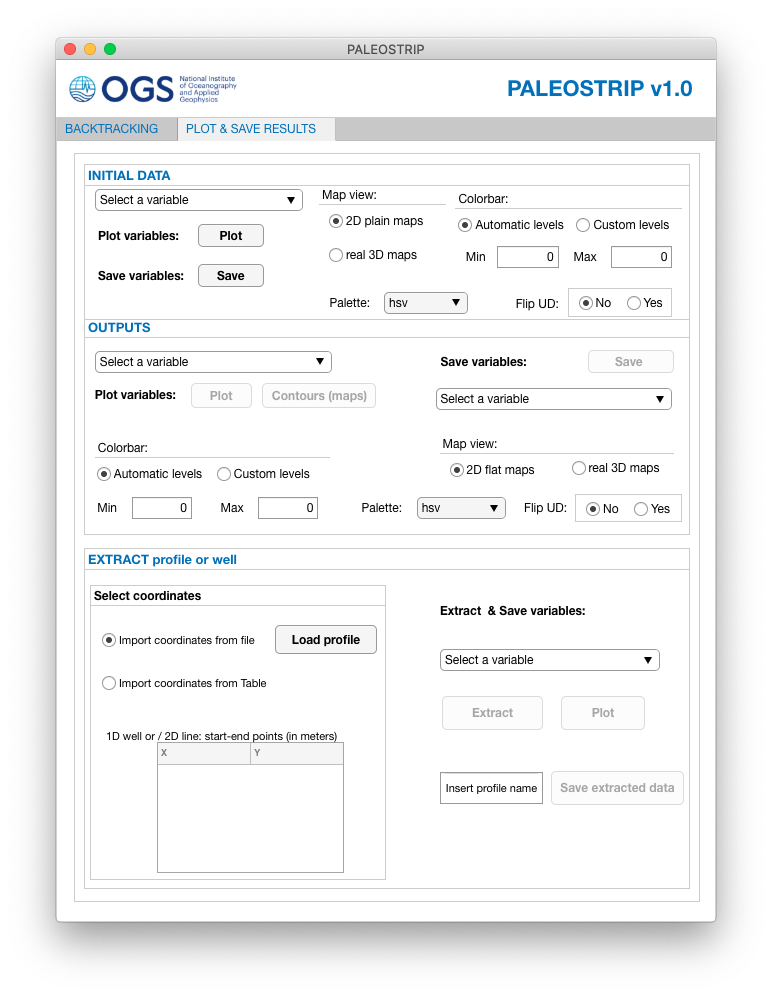
\includegraphics[width=\linewidth]{Figures/Fig_05_OUTPUTS_GUI.png}
\caption{PALEOSTRIP GUI - Plot \& Save outputs tab.}
\label{plot_gui}
\end{figure}

\subsubsection*{INITIAL DATA}

To check wether or not PALEOSTRIP red the input data in a proper way or to compare with backtracked output results, the first upper section \texttt{INITIAL DATA} allows the user to plot initial input data. Variables can be selected from the drop down menu:\\

\begin{itemize}
\item Horizon depths: Compacted sediment data from the input files.
\item Effective Elastic Thickness: if flexural isostasy with spatially variable Te has been selected.
\item Sea level correction: if switched on.
\item Spatially variable dynamic topography interpolated at input sediment layer ages.
\item Spatially variable or constant Beta factor.
\end{itemize}

The user can set several plot options:\\

\noindent \underline{Map view}: defines if the plot will draw a plain map or a map with 3D visual effect.\\

\noindent \underline{Colorbar}: Minimum and maximum values for the 2D plots or 2D maps can be automatically defined based on the minimum and maximum of input data (Automatic levels), or reset by the user on the GUI (Custom levels). Note that \textit{Min} and \textit{Max} needs to be indicated in the units of the selected variable.

\noindent \underline{Palette}:  a drop-down menu allows to chose 12 different colormaps, among which 3 from MATLAB defaults (hsv, jet and parula), 9 others are color-blind friendly and implemented from Crameri et al. (2020).

\noindent \underline{Flip UP}: this options allows the user to flip the colormap upside-down.  


\subsubsection*{OUTPUTS}
To plot the results from the backtracking, the variables can be selected from the drop-down menu: 
\begin{itemize}
\item Horizon depths: decompacted depths (m);
\item Isopachs: decompacted thicknesses (m);
\item Density: decompacted density (kg/cm3);
\item Porosity: decompacted porosity (\%);
\item Isostasy (m);
\item Thermal subsidence (m);
\item Tectonic: is the tectonic subsidence of the bedrock (in m), i.e. it corresponds to the bedrock backtracked depths at each time step and after the various corrections if switched on.
\end{itemize}

In the case of 3D backtracking, only the uppermost layer at each time step is plotted. In the case of 2D transects, all decompacted horizons depth are overimposed on the same plot for each time step of the backtracking procedure.\\

The user can set several plotting options that can be applied to both colormap plots or contour plots (\texttt{Contours (maps)} ):\\

\noindent \underline{Map view}: defines if the plot will draw a plain map or a map with 3D visual effect.\\

\noindent \underline{Colorbar}: Minimum and maximum values for the 2D plots or 2D maps can be automatically defined based on the minimum and maximum of input data (Automatic levels), or reset by the user on the GUI (Custom levels). Note that \texttt{Min} and \texttt{Max} needs to be indicated in the units of the selected variable.

\noindent \underline{Palette}:  a drop-down menu allows to chose 12 different colormaps, among which 3 from MATLAB defaults (hsv, jet and parula), 9 others are color-blind friendly and implemented from Crameri et al., (2020).

\noindent \underline{Flip UP}: this options allows the user to flip the colormap upside-down.  

\clearpage
\newpage

\section{Save outputs}\label{saveout}

The user can select a backtracked variable from drop down menu among:
\begin{itemize}
\item Horizon depths: decompacted depths (m);
\item Isopachs: decompacted thicknesses (m);
\item Density: decompacted density (kg/cm3);
\item Porosity: decompacted porosity (\%);
\item Isostasy (m);
\item Thermal subsidence (m);
\item Tectonic(m).
\end{itemize}

By clicking on \texttt{Save}, the backtracked data are saved in ASCII format in the selected directory with a filename defined as:
\begin{verbatim}
       HORIZON_NAME_backstripped_depths_runid.dat
       HORIZON_NAME_backstripped_isopachs_runid.dat
       HORIZON_NAME_backstripped_density_runid.dat
       HORIZON_NAME_backstripped_porosity_runid.dat
       HORIZON_NAME_thermal_subs_correction_runid.dat
       HORIZON_NAME_isostatic_correction_runid.dat
       HORIZON_NAME_tectonic_subsidence_runid.dat 
\end{verbatim}

\noindent Output files contain the depths of all remaining horizons at each backtracked time steps and written in the ASCII file from \textbf{\textcolor{red}{top to bottom}} (from the bathymetry to the basement). \\

\noindent Output files thus contain n columns: if 2D or 3D, the first and/or second columns correspond to input cartesian coordinates X, Y, and the remaining columns correspond to the backtracked depths of horizons. For example:\\

\noindent \underline{Step 0: present-day (no backtracked):} \\
File1.dat: [X and/or Y] [horizon09\_depth]  [horizon08\_depth]  [horizon07\_depth] ... [horizon01\_depth]\\

\noindent \underline{Step 1 (1 layer removed):} \\
File2.dat: [X and/or Y] [horizon08\_depth]  [horizon07\_depth]  ... [horizon01\_depth]\\

\noindent \underline{Step 2 (2 layer removed):} \\
File3.dat: [X and/or Y] [horizon07\_depth]  ... [horizon01\_depth]
...\\

\textcolor{blue}{\noindent Hint: the \texttt{HORIZON\_NAME} string in the file name refers to the uppermost horizon written in the files at each timestep.}



%------------ EXTRACT SECTIONS AND WELLS
\clearpage
\newpage

\section{Extract 2D sections and wells from backtracked outputs}\label{sec:extract}

PALEOSTRIP provides several two ways to extract transects or wells from backtracked 2D transects or 3D maps:\\

\subsection*{Import coordinates}
\noindent \underline{Import coordinates from files}: allows to upload a X,Y transect along which backtracked data will be extracted. \textbf{Note that X,Y coordinates must be cartesian coordinates with the same geographical projection than backtracked/input sediment data}. Data at each X,Y point are extracted using the \textit{scatterInterpolant} function that linearly interpolates backtracked points onto the input coordinates. No extrapolation is allowed outside the backtracked data polygon/grid.\\

\noindent \underline{Import coordinates from Table}: allows the user to prescribe a starting point (X,Y) and end point (X,Y) of a 2D transect or only a single point (X,Y) in case of a 1D well. For the 2D transect, 500 points are linearly interpolated between starting point and end point and backtracked data are extracted at those interpolated coordinates. \textbf{Note that X,Y coordinates must be cartesian coordinates with the same geographical projection than backtracked/input sediment data}. (X,Y) points can be retrieved on the Matlab plots of backtracked results. \\

\textit{\textcolor{blue}{Hint: In the \textit{Tool} menu, the \textit{Data Tip} option allows the user to use the mouse and to point on the figure to retrieve the value of X,Y coordinates at a single grid point.}}\\

\subsection*{Extract data}
Once the coordinates are loaded or prescribed, the user can use the drop menu to select the variable to be extracted among:
\begin{itemize}
\item Horizon depths (m);
\item Isopachs (m);
\item Density;
\item Porosity;
\item Thermal subsidence;
\item Isostasy;
\item Beta Factor;
\item Tectonic (m)
\end{itemize}

\noindent and click on \textbf{Extract}.\\

\noindent If the extraction is successful, the user can plot the extracted 2D transect or 1D well by clicking on \textbf{Plot}.\\

\subsection*{Save extracted data}
\noindent Extracted data can be saved by indicating a string that will be concatenated to the file name and by clicking on \textbf{Save extracted data}. Format follows that described in section~\ref{saveout}.



%-----------------------------------------------------------
% PRE-PROCESSING OF USER DATA
%-----------------------------------------------------------
\chapter{Pre-processing of user-based data}\label{preproc}
\section{Geographical coordinates}\label{sec:coordinates}

PALEOSTRIP exclusively works with cartesian coordinates, this is to allow flexural isostasy. \textcolor{red}{\textbf{PALEOSTRIP does not convert geographical coordinate into cartesian coordinates}}. The user might use different GIS softwares, or GMT, Python or Matlab tools or any other ways to prepare all the input files.

\section{Files format}\label{format}

All input and output files are in ASCII format. The current PALEOSTRIP release v1.0 does not accept NetCDF format.\\

\begin{tcolorbox}[colback=GreenYellow]
\textbf{IMPORTANT:} 
\begin{itemize}
\item \textbf{The user must provides present-day bathymetry and depth of the basement.}
\item \textbf{The files containing the horizons depths must have the extention \textcolor{red}{.dat}}
\item \textbf{The files needs to be numerated from \textcolor{red}{bottom to top}, thus from 1 (basement depth) to ...N (bathymetry).}
\item \textbf{All input horizons depth files must have the \textcolor{red}{same length} or the same grid extent and resolution.}
\item \textbf{Cartesian coordinates (for 2D and 3D) and horizon depths need to be provided in meters.}
\item \textbf{Lithological parameters needs to be provided in a separated ASCII file with the extention \textcolor{red}{.par}. See Section~\ref{lithopar}.}
\end{itemize}
\end{tcolorbox}

\clearpage
\newpage

\subsection{1D: wells}
Files for 1D wells must contain only \textcolor{red}{\textbf{1 column}}: the (present-day) compacted horizons depth.\\

\noindent Example of horizon file (*.dat) - No headers:\\

\begin{Verbatim}[frame=single]
3396
\end{Verbatim}

If the well includes several sediment layers to be decompacted, then the horizons depth must be provided in separated ASCII files.\\

\underline{Example}: a well with 6 horizons will results in 6 separated files, each containing one value of the horizon depth. But the \textbf{total number of files} to be provided to PALEOSTRIP will be \textbf{9}: 
\begin{itemize}
\item the 6 separated horizons depths; 
\item one file with present-day bathymetry; 
\item one file with a basement layer depth; 
\item a lithological parameter file (see Section~\ref{lithopar}).
\end{itemize}


\clearpage
\newpage

\subsection{2D: transect}

Files for 2D transect must contain \textcolor{red}{\textbf{2 columns}}: X coordinates (or Y) in meters and the (present-day) compacted horizons depth (in meters). \\

\noindent Example of horizon file (*.dat) - No headers:\\

\begin{Verbatim}[frame=single]
4786000.000000 2564.0099
4787000.000000 2544.3365
4788000.000000 2524.2541
4789000.000000 2504.0505
4790000.000000 2484.0203
4791000.000000 2461.9670
4792000.000000 2425.0767
...
\end{Verbatim}

Note that the transect can vary more along the X direction than along the Y direction or vice-versa. In the case the distance varies mainly along the X direction, then the input file will contain (X ; DEPTHS).\\

If the transect includes several sediment layers to be decompacted, then the horizons depth must be provided in separated ASCII files. \\
\underline{Example}: a transect with 6 horizons will results in 6 separated files, each containing one value of the horizon depth. But the \textbf{total number of files} to be provided to PALEOSTRIP will be \textbf{9}:
\begin{itemize}
\item the 6 separated horizons depths; 
\item one file with present-day bathymetry; 
\item one file with a basement depth; 
\item a lithological parameter file (see Section~\ref{lithopar}).
\end{itemize}



\clearpage
\newpage

\subsection{3D: maps}
Files for 3D maps must contain \textcolor{red}{\textbf{3 columns}}: X and Y coordinates in meters and the (present-day) compacted horizons depth (in meters). \\

\noindent Example of horizon file (*.dat) - No headers:\\

\begin{Verbatim}[frame=single]
4592400.000000 3499200.000000 6612.1426
4592400.000000 3497200.000000 6631.5210
4592400.000000 3495200.000000 6649.9180
4592400.000000 3493200.000000 6667.8740
4592400.000000 3491200.000000 6685.7744
...
\end{Verbatim}

Note that the maps of the horizon depths \textbf{can be provided on a non rectangular grid}. PALEOSTRIP creates the rectangular grid during the flexure calculation automatically using the horizontal resolution of the input maps. However, although the shape of the grid can be an irregular polygon, \textbf{the horizontal resolutions $dx$ and $dy$ must be regular} but $dx$ can differ from $dy$.\\

If the area include several sediment layers to be decompacted, then the horizons depth must be provided in separated ASCII files. \\
\underline{Example}: a map with 6 horizons will results in 6 separated files, each containing one value of the horizon depth. But the \textbf{total number of files} to be provided to PALEOSTRIP will be \textbf{9}:
\begin{itemize}
\item the 6 separated horizons depths; 
\item one file with present-day bathymetry; 
\item one file with a basement depth; 
\item a lithological parameter file (see Section~\ref{lithopar}).
\end{itemize}


\clearpage
\newpage

\subsection{Lithological parameters}\label{lithopar}

There are three lithological parameters needed by PALEOTRIP together with other properties of the horizons*:
\begin{itemize}
\item \textbf{LAYER} (integer): horizon number from bottom to top. Note that bathymetry is not specified within this file (see below).
\item \textbf{POROSITY} (float): Surface deposition porosity (in percent, decimal)
\item \textbf{DEC COEF} (float): Decompaction coefficient (km$^{-1}$)
\item \textbf{DEN} (float): Dry Density (kg/m${-3}$)
\item \textbf{AGE} (float): age of horizons in Million years ago (Ma)
\item \textbf{NAME} (string): name of the horizons/unconformities
\end{itemize}

*Horizons correspond to boundary layers (example: lithological changes or seismic reflectors, etc...).\\\\


\noindent Example of lithological parameter files (*.par):

\begin{Verbatim}[frame=single]

NUMBER OF LAYERS =           9

  LAYER  POROSITY   DEC COEF  DEN  AGE BASE     NAME
                    (1/KM)   (KG / MC)   (MA)

  1    0.4900    0.2700    2680.00    34.00   basamento
  2    0.4500    0.4500    2680.00    26.00   rsu_6
  3    0.4500    0.4500    2680.00    24.90   rsu_5b
  4    0.4500    0.4500    2680.00    19.70   rsu_5a
  5    0.4500    0.4500    2680.00    18.00   rsu_5
  6    0.4500    0.4500    2680.00    14.20   rsu_4
  7    0.4500    0.4500    2680.00    10.00   rsu_3
  8    0.4500    0.4500    2680.00    4.00    rsu_2
  9    0.4500    0.4500    2680.00    0.60    rsu_1
\end{Verbatim}


\begin{tcolorbox}[colback=GreenYellow]
\textbf{The lithological parameters file must strictly respect this format:} 
\begin{itemize}
\item \textbf{line 1}: blank line
\item \textbf{line 2}: number of layers (integer)
\item \textbf{line 3-6}: blank line; headers (2 lines); blank line
\item \textbf{line 7 and onward}: parameters values
\item \textbf{format of parameters}: \%d \%f \%f \%f \%f \%s
\end{itemize}
\end{tcolorbox}



\clearpage
\newpage

\subsection{Files name and numbering}

Input files name must follow the format:

\begin{verbatim}
Prefix_nbLayer_HORIZON_NAME.dat
Prefix.par
\end{verbatim}

Filenames for input horizons depth must start with the same prefix, followed by the number of the layer and ending by a string name (freely provided) by the user. A typical input data directory looks like:

\begin{Verbatim}[frame=single]
RS.par
RS_01_Basement.dat
RS_02_RSU4.dat
RS_03_Bathymetry.dat
Dynamic_Topo_Muller_et_al_2018/
Variable_Te_Chen_et_al_2018/
\end{Verbatim}

A directory can contain other sub-directories, but cannot contain multiple parameter files, for example with:
\begin{Verbatim}[frame=single]
RS.par
RS_litho2.par
RS_01_Basement.dat
RS_02_RSU4.dat
RS_03_Bathymetry.dat
Dynamic_Topo_Muller_et_al_2018/
Variable_Te_Chen_et_al_2018/
\end{Verbatim}

\noindent PALEOSTRIP will issue the follow \textcolor{red}{\textbf{error message}}:

\begin{verbatim}
``The folder must contain exactly one parameter file.''
\end{verbatim}

\noindent If the wrong number of layers is indicated within the lithological parameter file \texttt{*.par}, PALEOSTRIP will issue the follow \textcolor{red}{\textbf{error message}}:
\begin{verbatim}
``The folder must contain a .dat file per layer and a .dat file for the bathymetry.''
\end{verbatim}

%-----------------------------------------------------------
%APPENDIX A
%-----------------------------------------------------------
\chapter{Appendix A}

In this appendix, we provide visual examples on running PALEOSTRIP for 1D, 2D and 3D backtracking.

Start MATLAB and enter PALEOSTRIP directory:

\begin{figure}[!h]
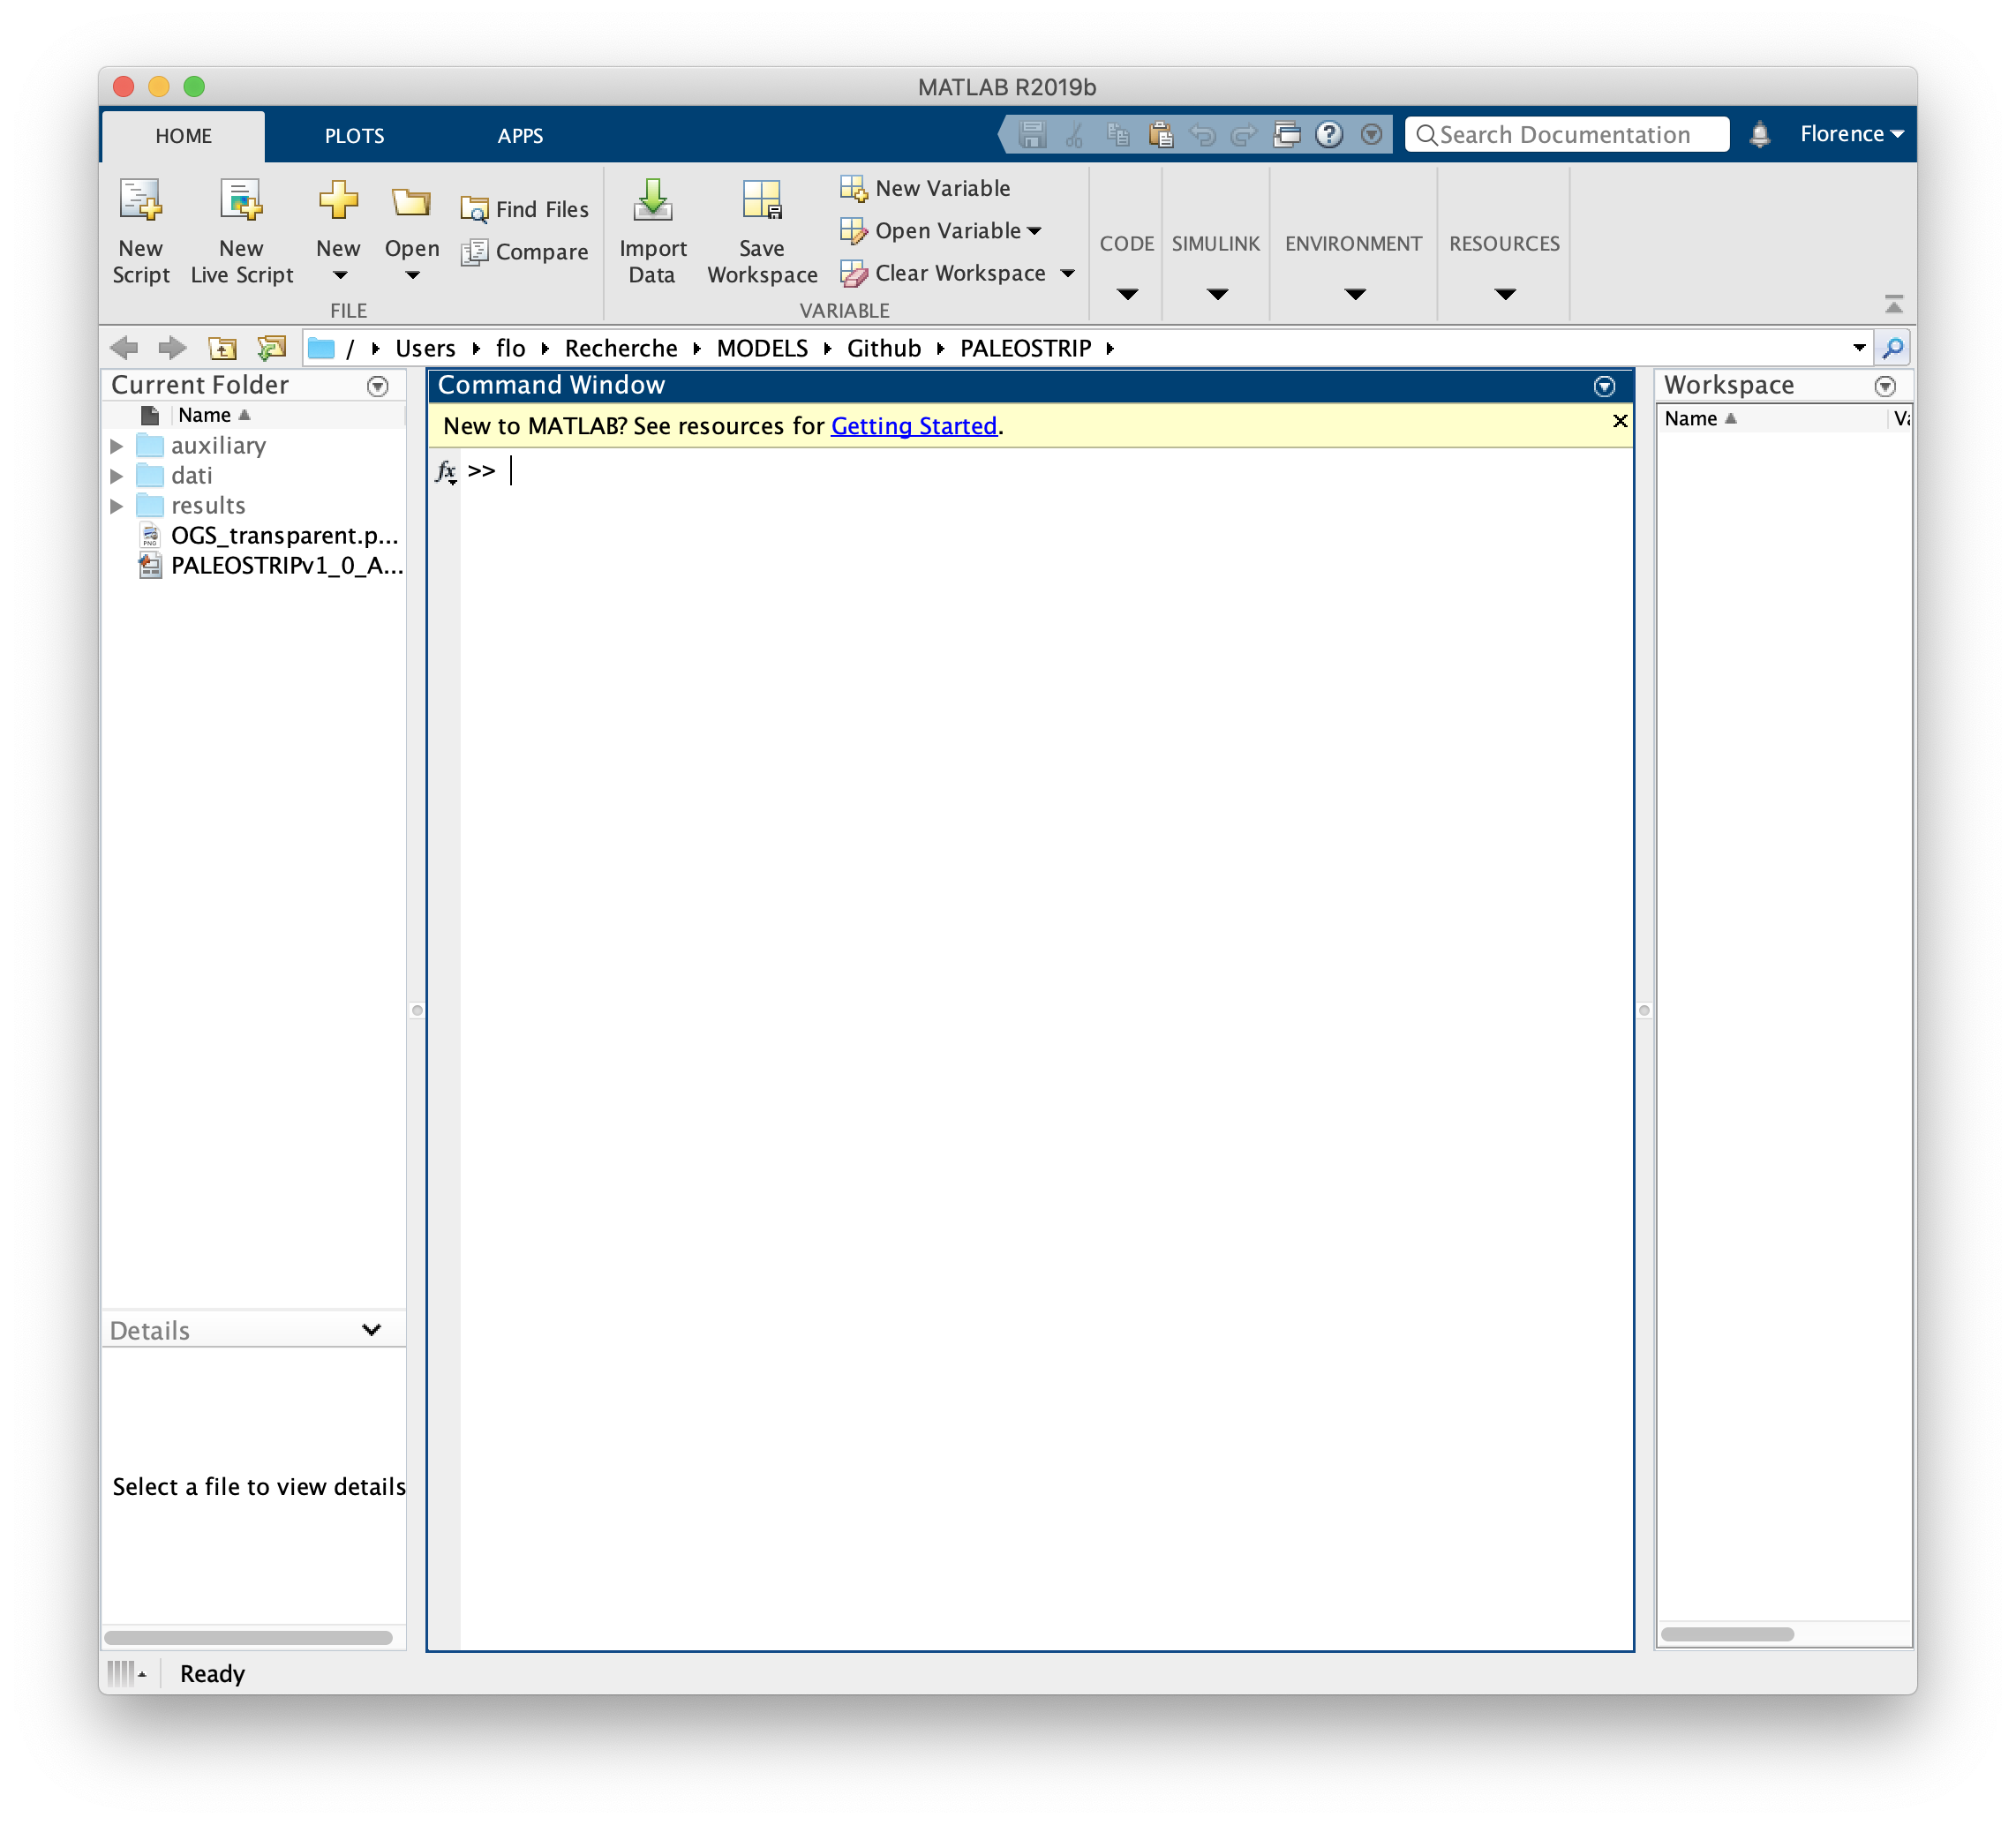
\includegraphics[scale=0.4]{Figures/1D/MATLAB_interface.png}
\end{figure} 

\section{1D well}

\subsection*{1- Import data}

Once data are loaded, the lithological parameters values are listed in the Table in the middle of the GUI.

\begin{figure}[!h]
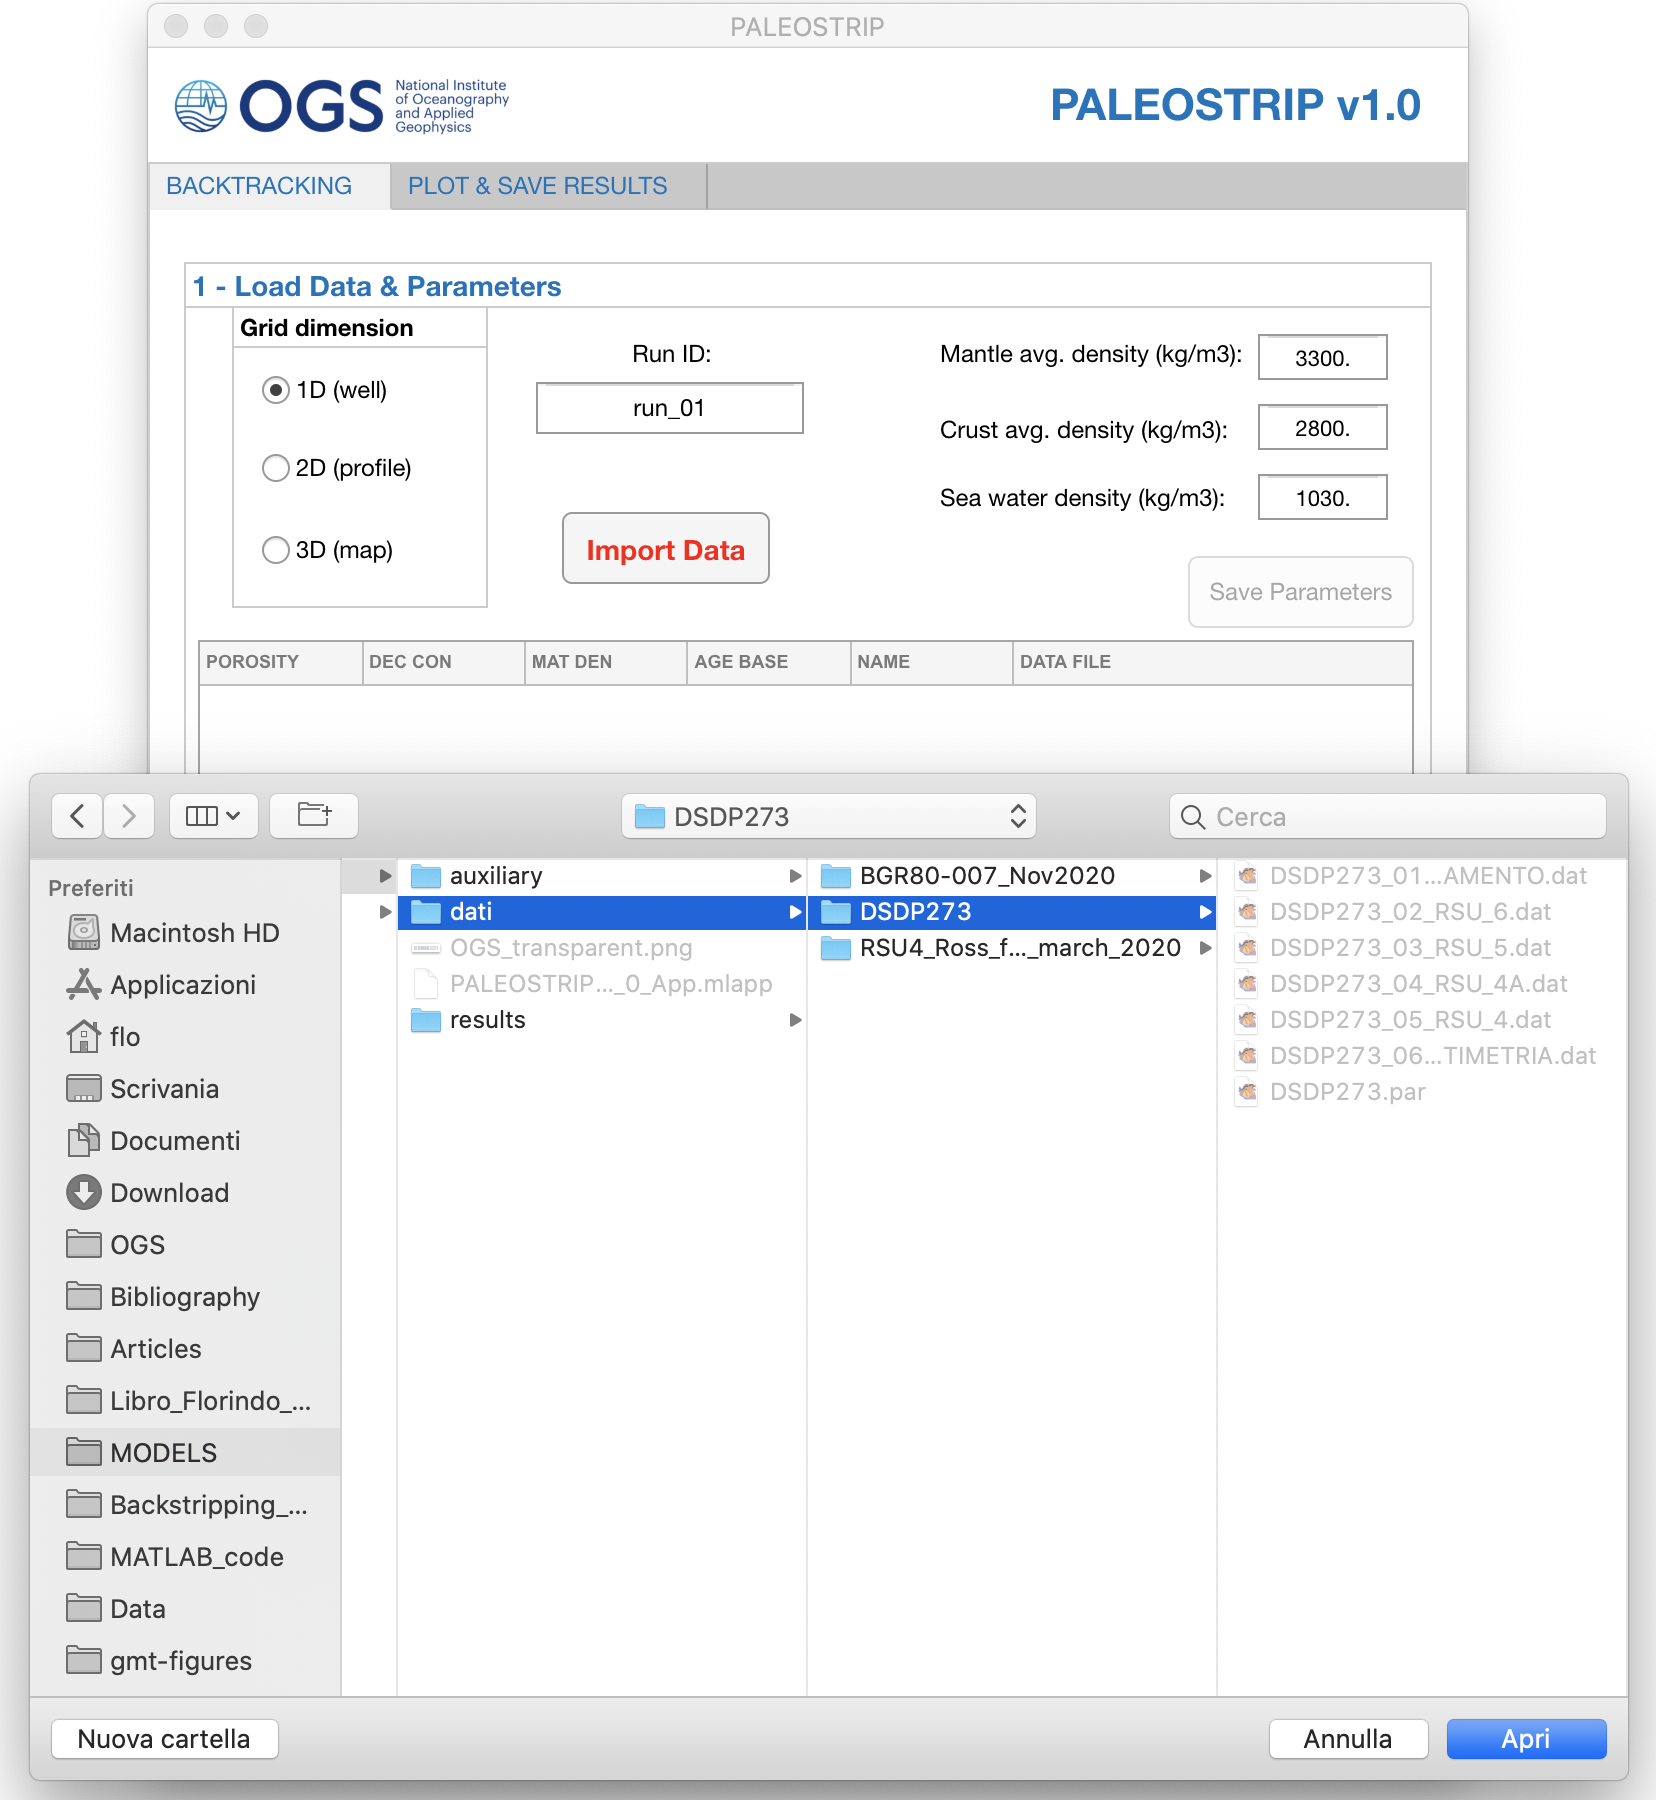
\includegraphics[scale=0.3]{Figures/1D/Import_data_1D.png}
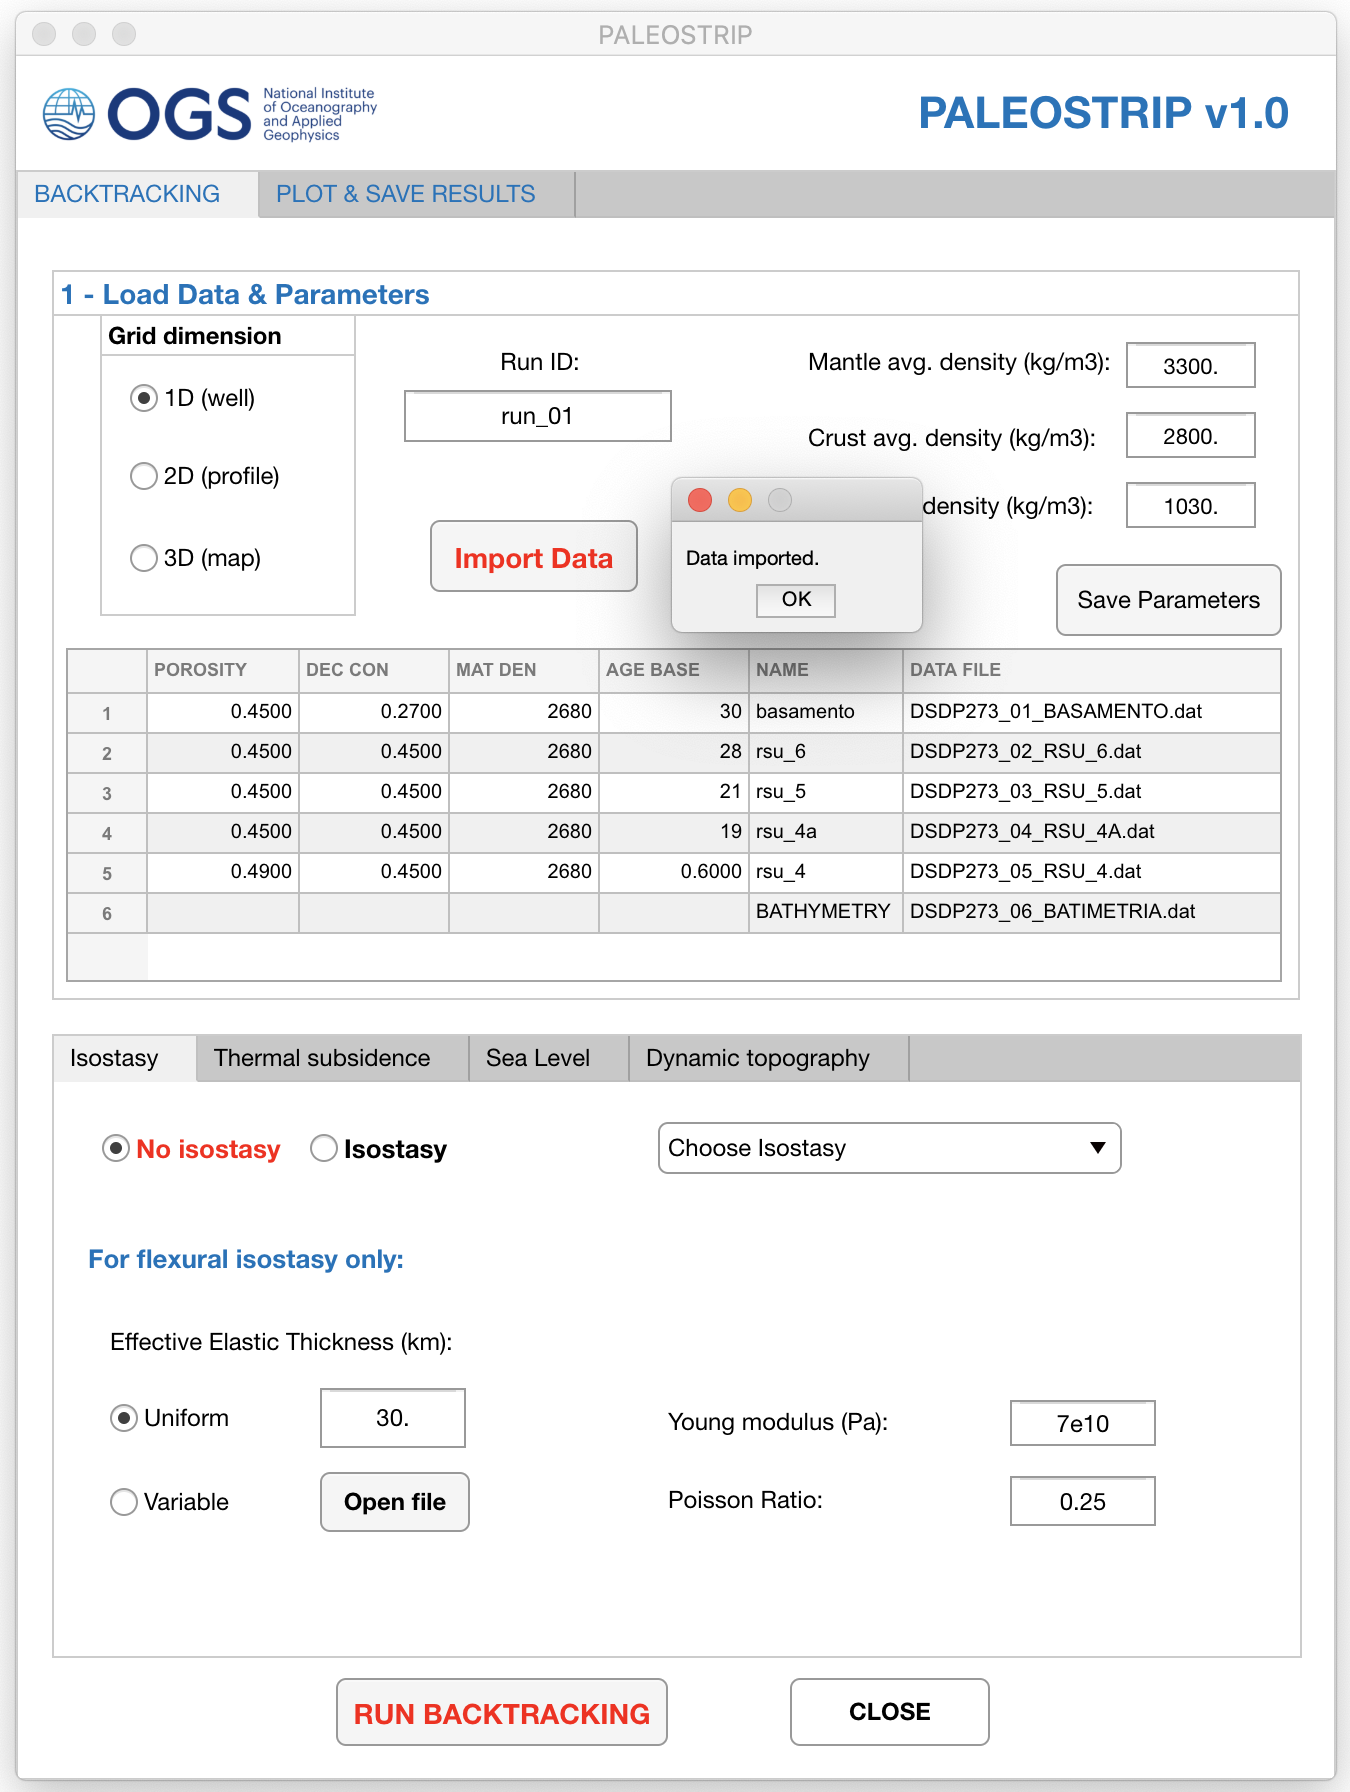
\includegraphics[scale=0.3]{Figures/1D/Data_imported_OK.png}
\caption{Load data from directory by clicking on \textbf{\textcolor{red}{Import Data}}. Data Loading successful.}
\end{figure} 

\clearpage
 \newpage
\subsection*{2- Select physical parameters and corrections}

\begin{figure}[!h]
\includegraphics[scale=0.4]{Figures/1D/isostasy.png}
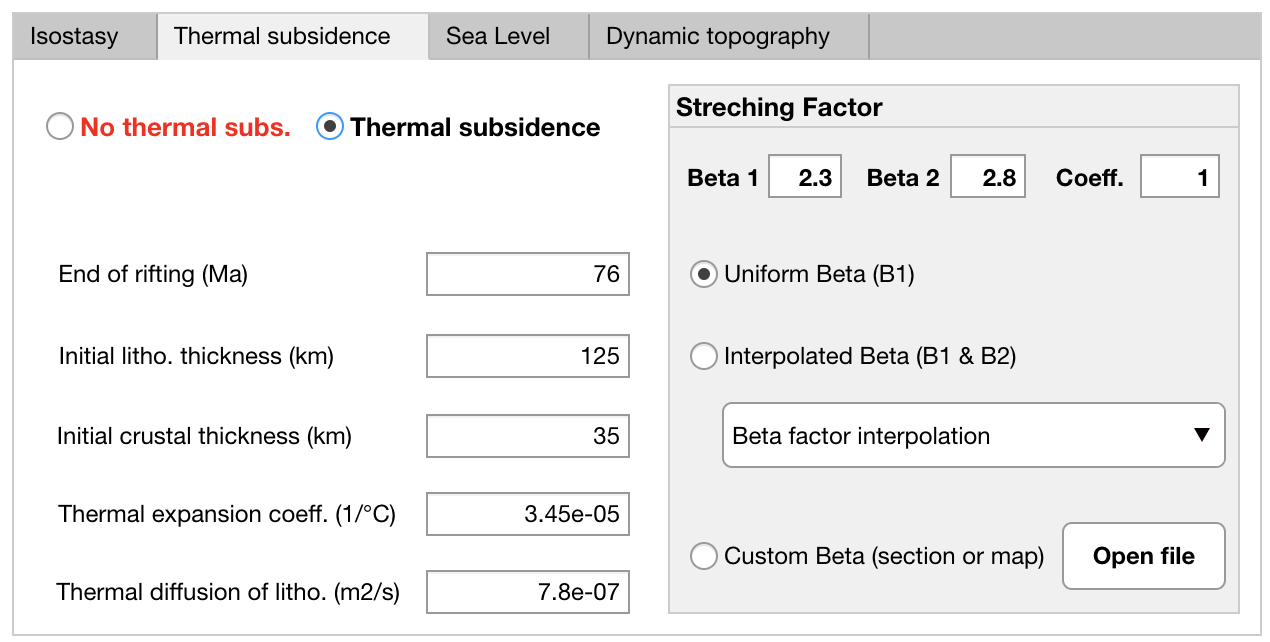
\includegraphics[scale=0.4]{Figures/1D/Thermal_subsidence.png}\\
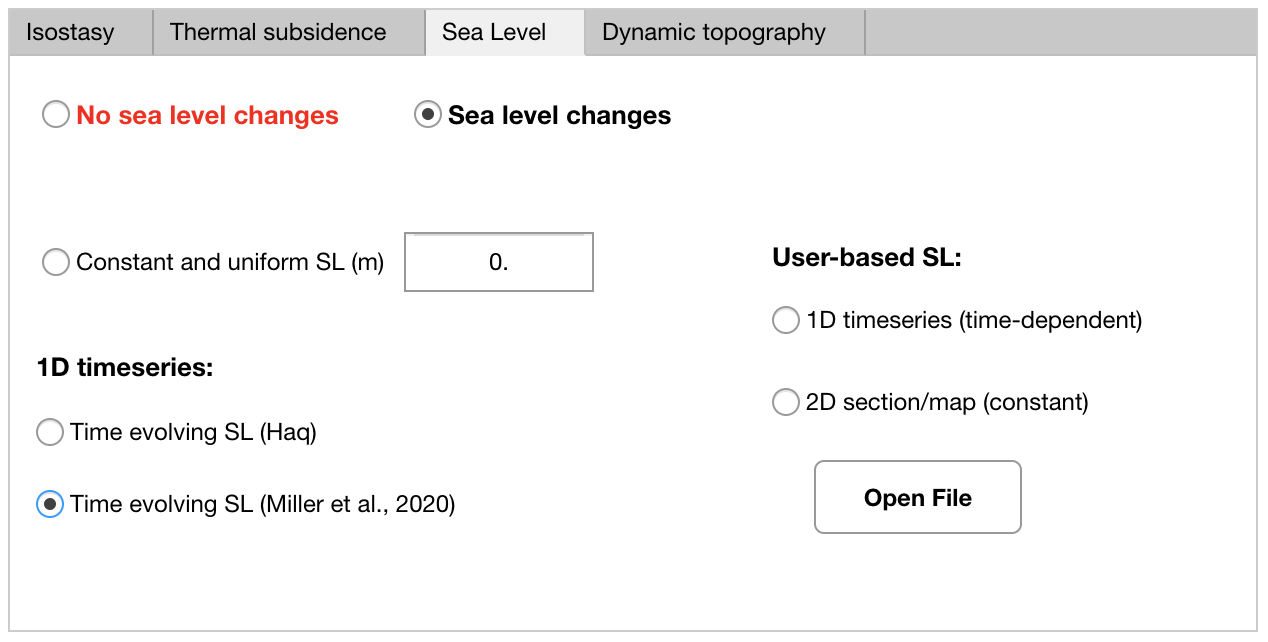
\includegraphics[scale=0.4]{Figures/1D/Sea_Level.png}
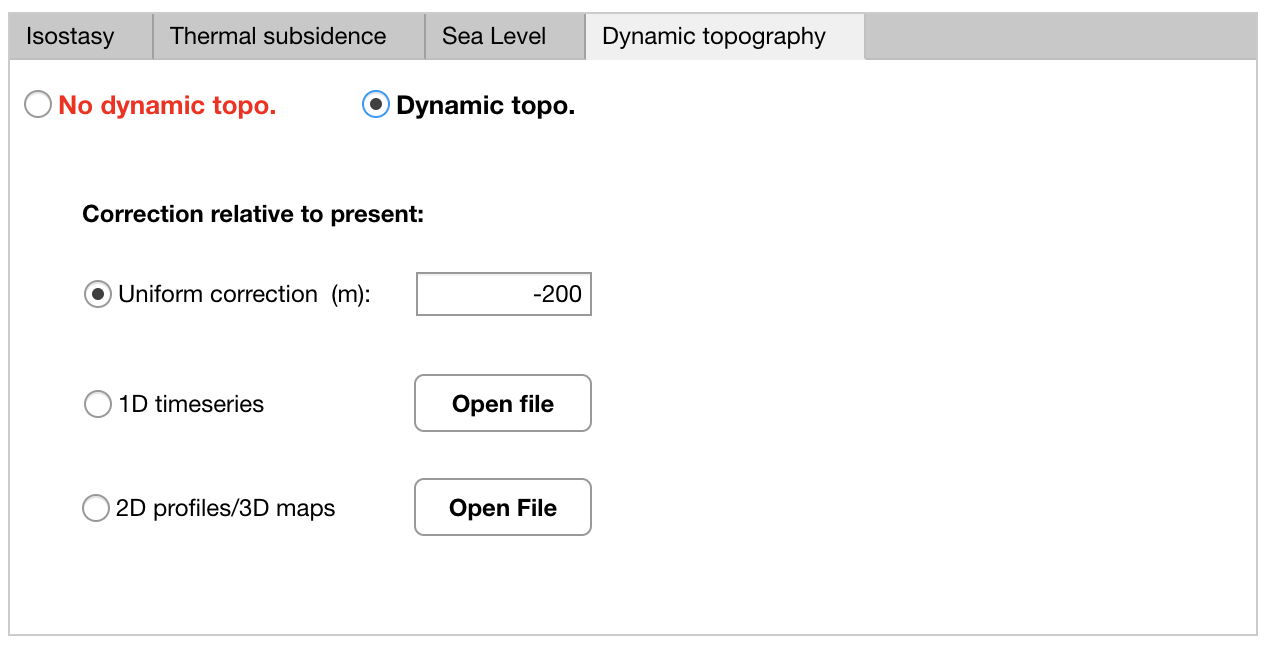
\includegraphics[scale=0.4]{Figures/1D/Dynamic_topography.png}
\caption{For 1D well: only Airy isostasy will be allowed. In the example we use fixed Beta factor (so only B1 value will be accounted for). We use 1D sea level changes from Miller et al., 2020 timeseries. We use a spatially uniform and constant dynamic topographic correction. Prescribed value is ad-hoc. }
\end{figure} 


\clearpage
\newpage
\subsection*{3- Run Backtracking}

Click on \textbf{\textcolor{red}{Backtracking}}. If everything is successful, you got the dialog message \texttt{Decompaction completed}.

\begin{figure}[!h]
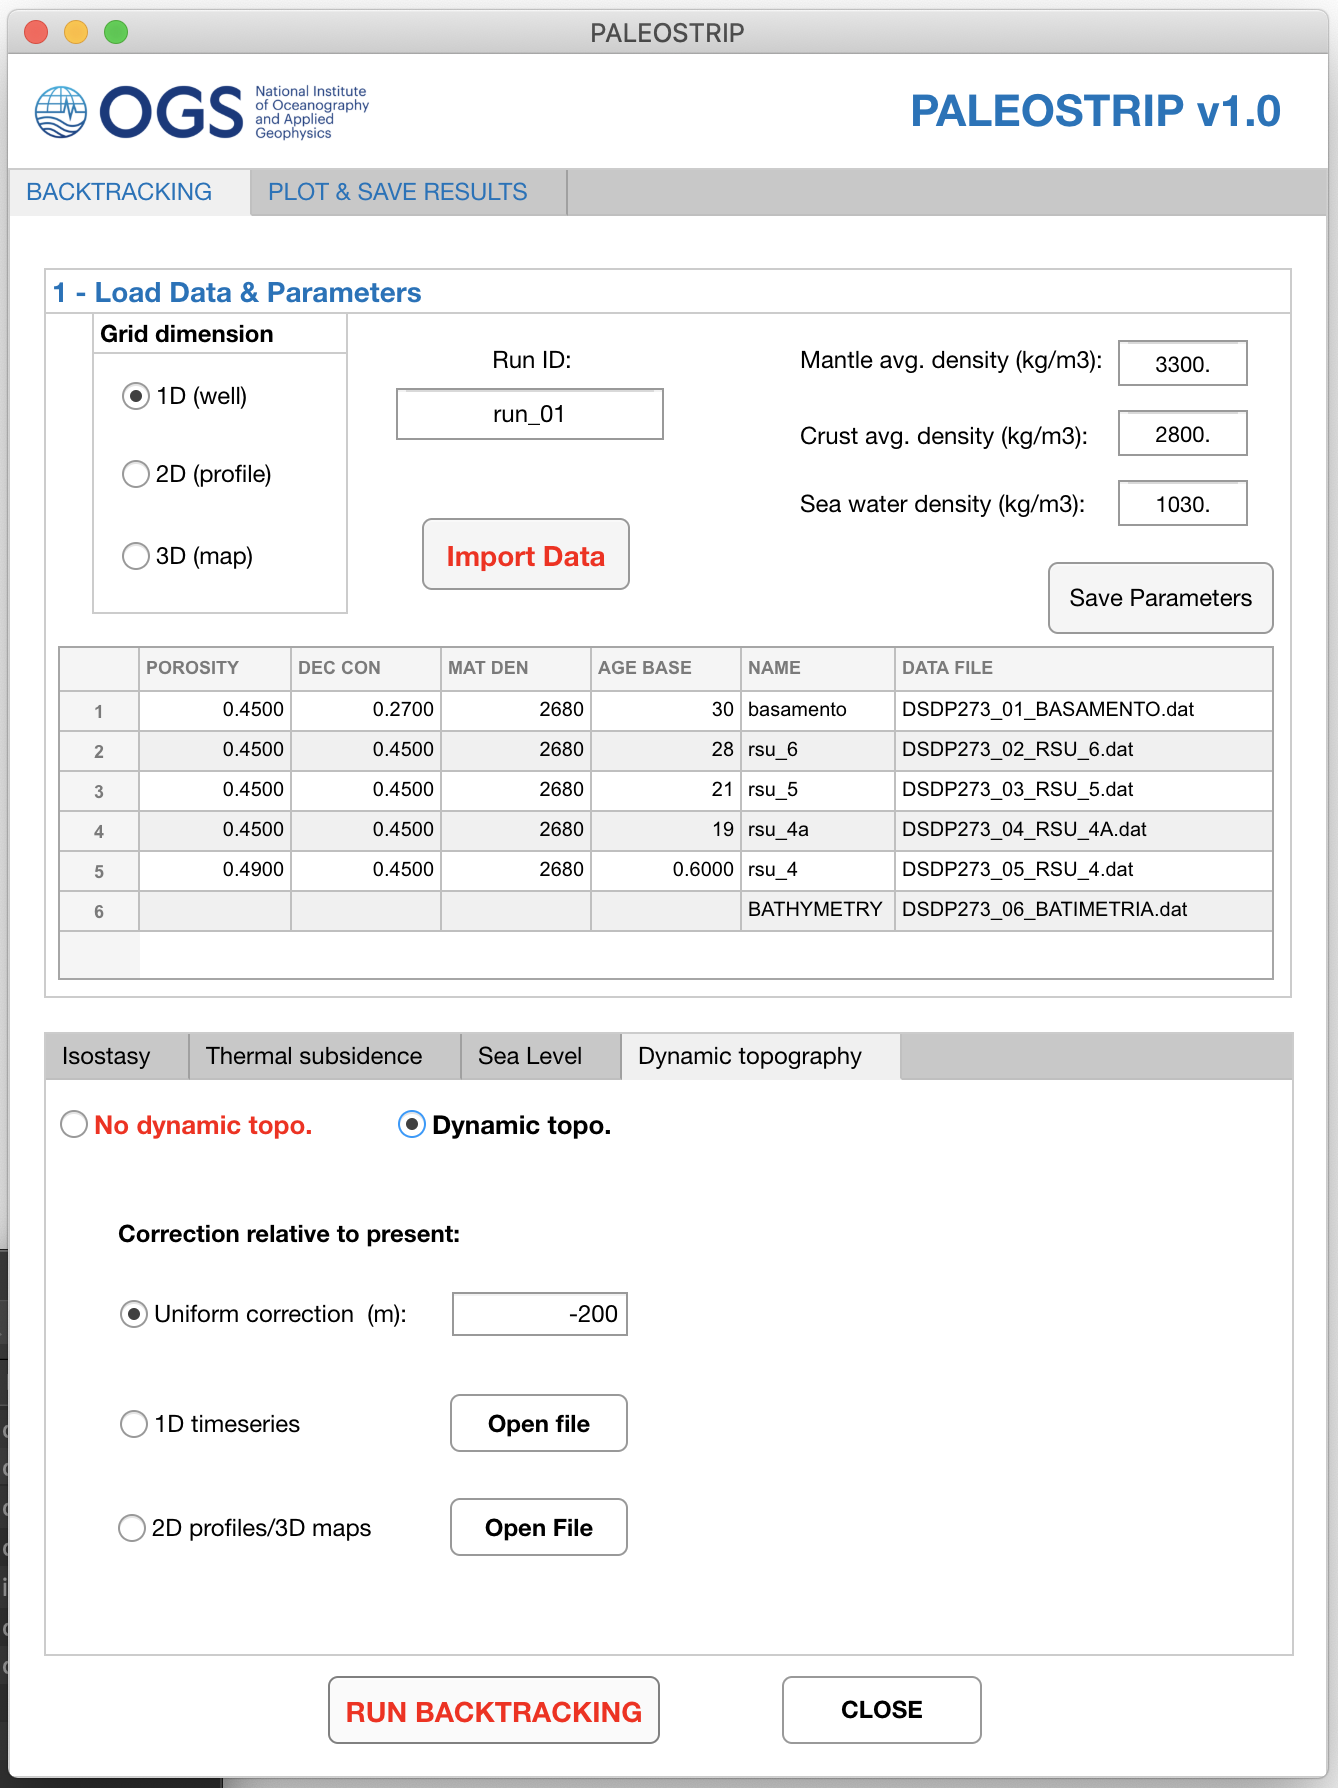
\includegraphics[scale=0.35]{Figures/1D/PALEOSTRIP_GUI.png}
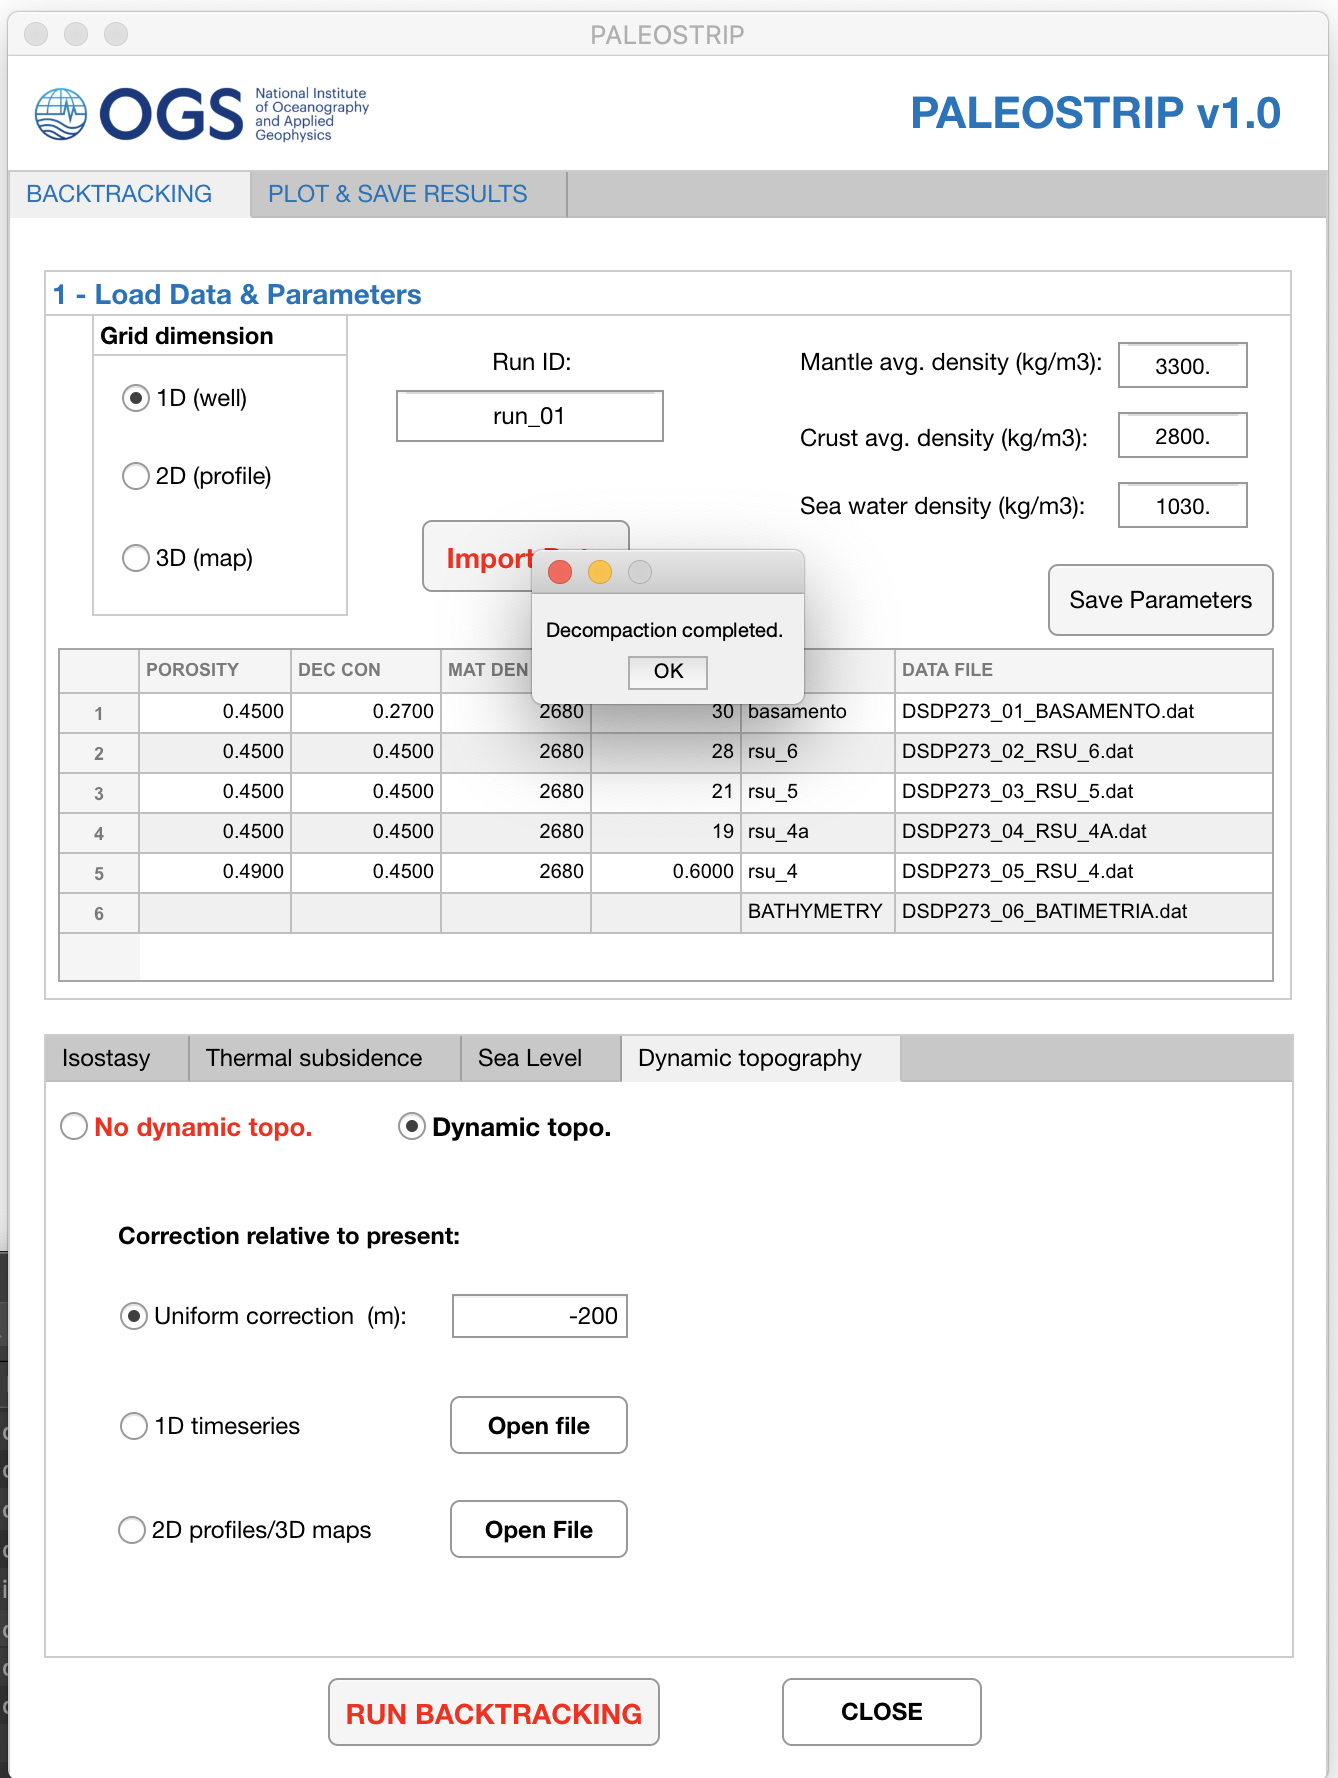
\includegraphics[scale=0.35]{Figures/1D/Decompaction_OK.png}
\end{figure} 


\clearpage
\newpage
\subsection*{4- Plot outputs}
The user can check if PALEOSTRIP read your input data correctly by plotting initial horizon depths:

\begin{figure}[!h]
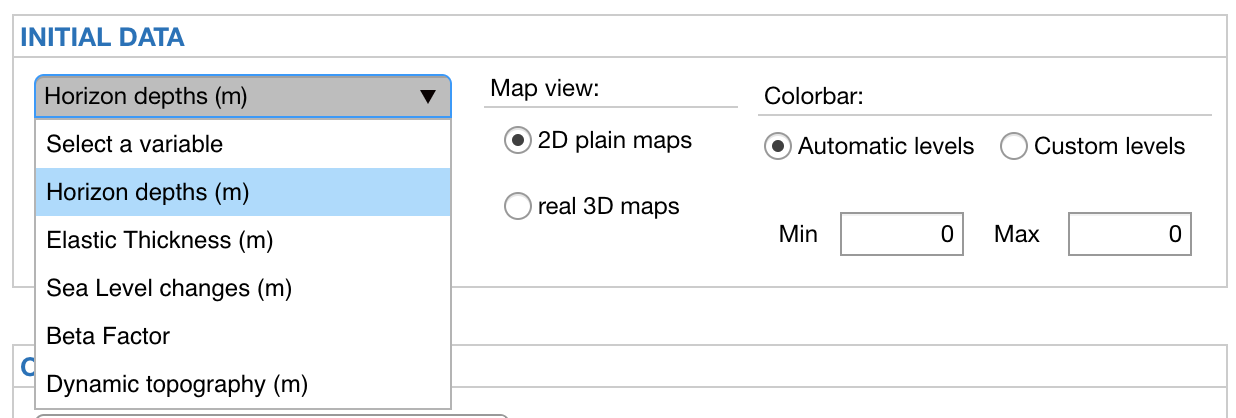
\includegraphics[scale=0.35]{Figures/1D/Initial_data_select.png}\\\\
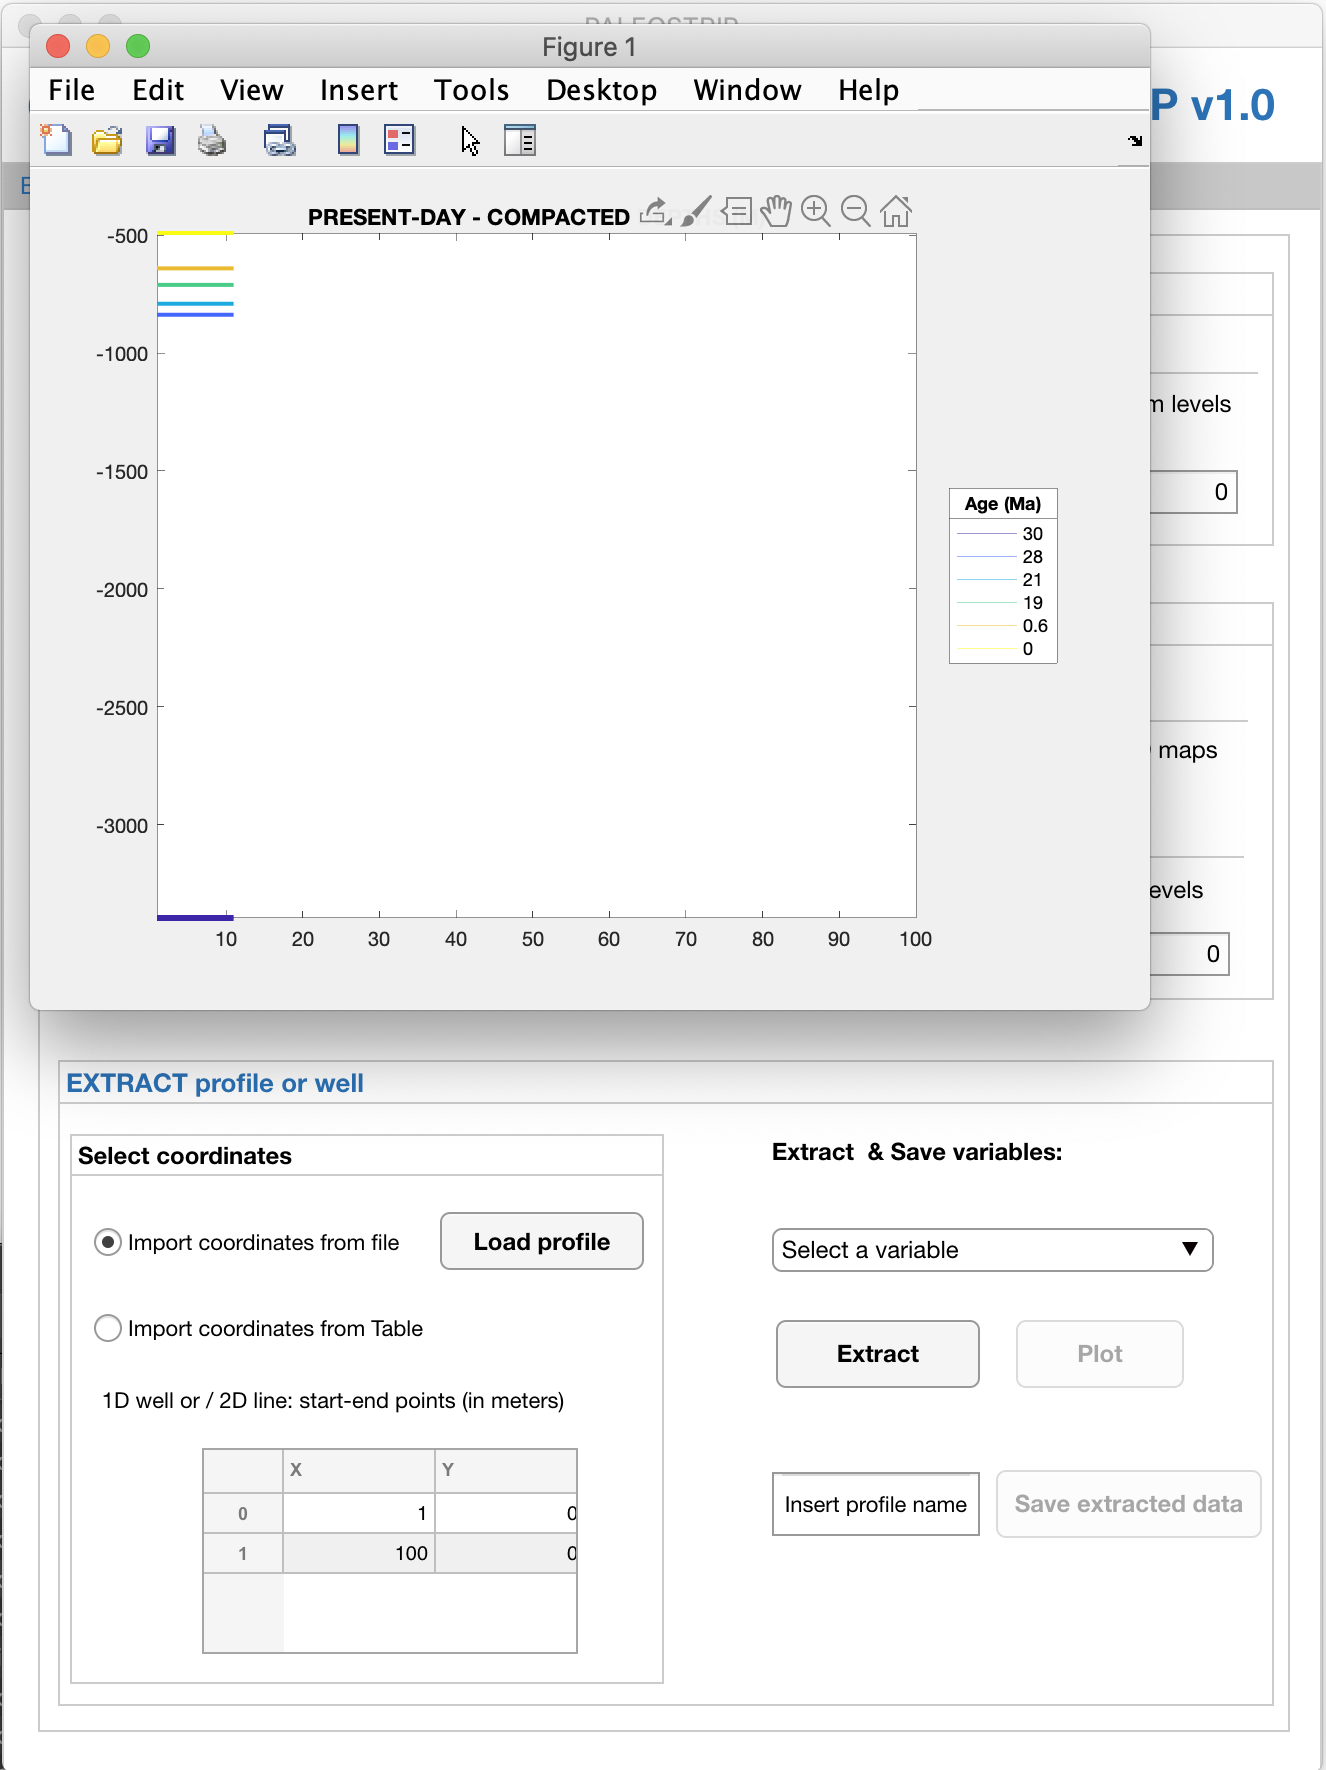
\includegraphics[scale=0.35]{Figures/1D/Initial_data_plot.png}
\end{figure}

This step is not mandatory to plot backtracked variables.\\

To plot outputs variables, the use can select them from the drop-menu and then click on \texttt{Plot}. In 1D, the custom options are not allowed:

\begin{figure}[!h]
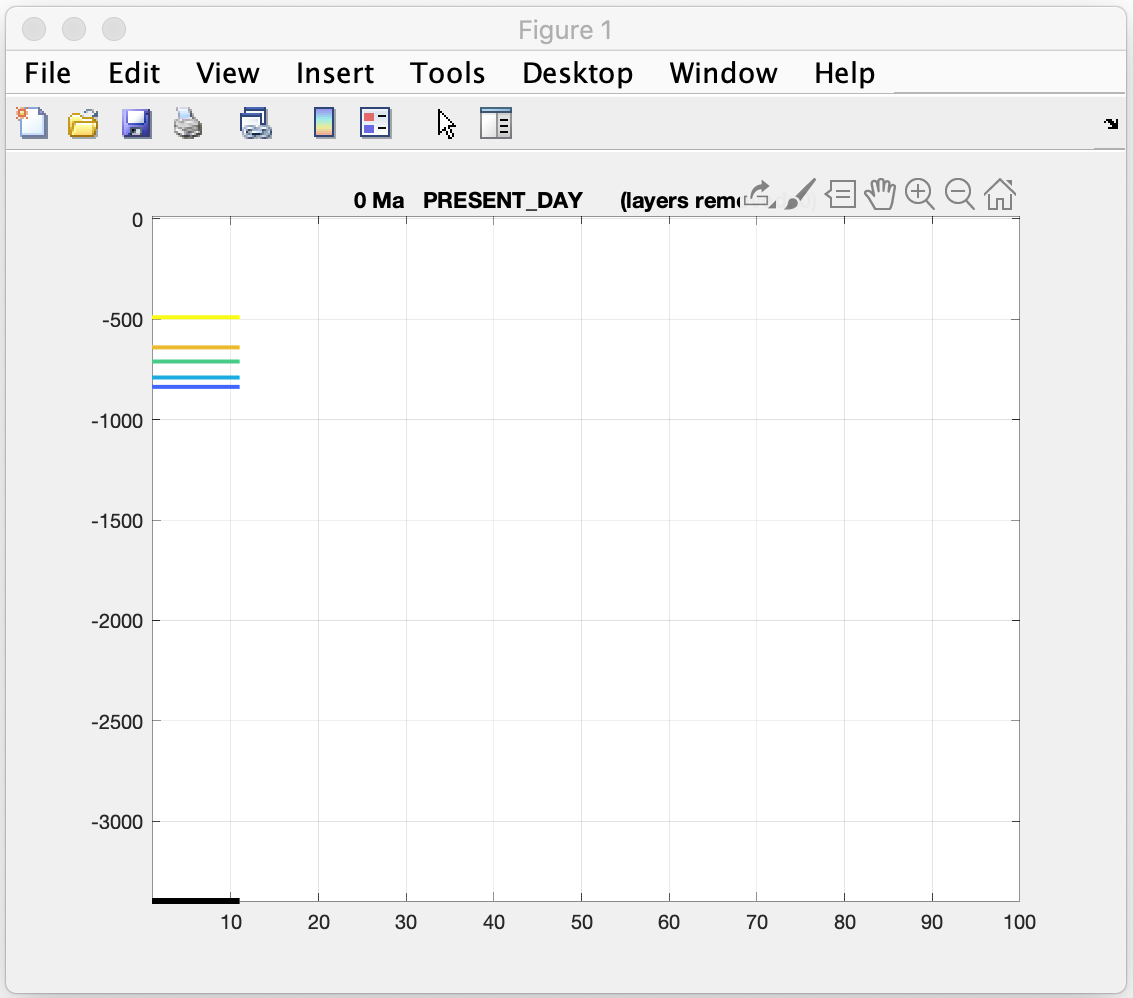
\includegraphics[scale=0.35]{Figures/1D/H06.png}
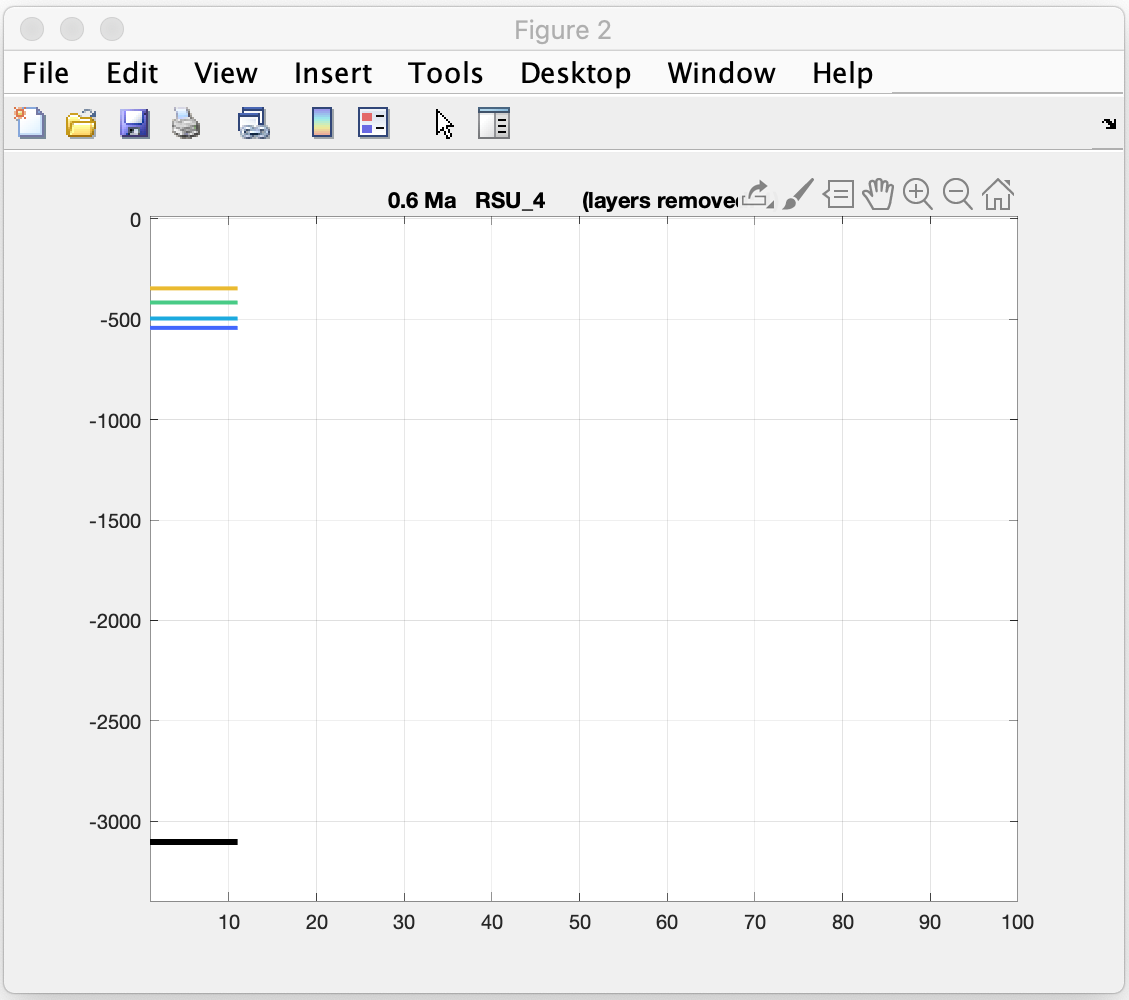
\includegraphics[scale=0.35]{Figures/1D/H05.png}\\
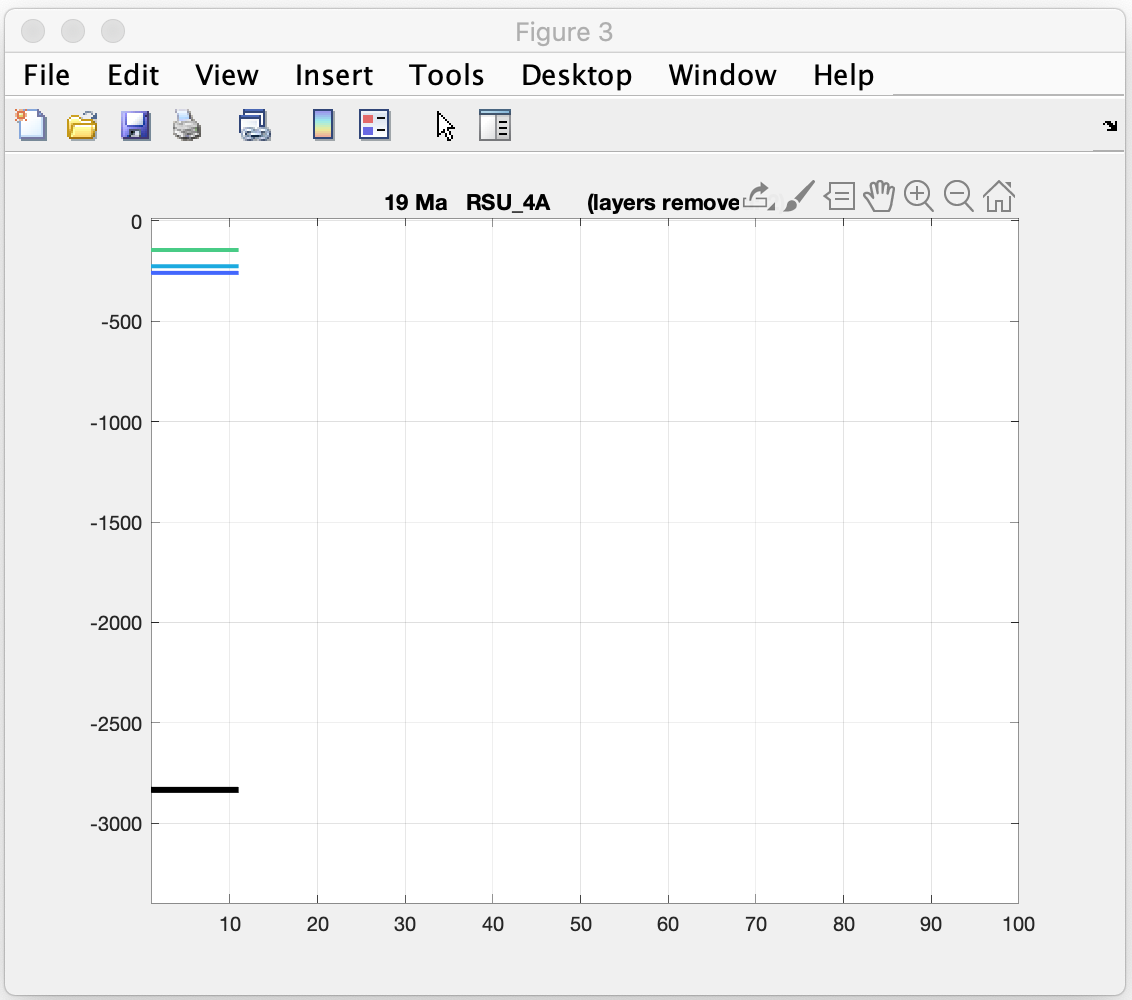
\includegraphics[scale=0.35]{Figures/1D/H04.png}
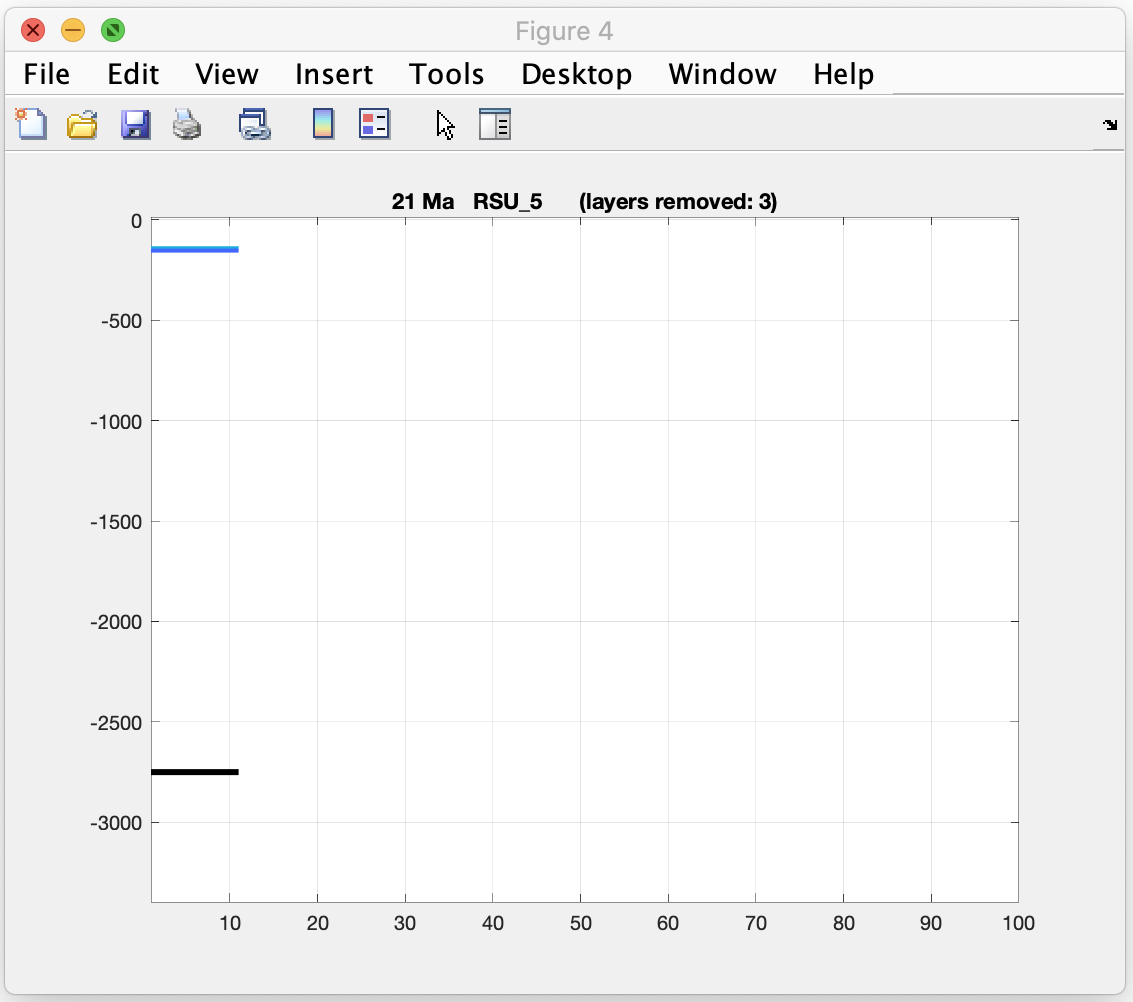
\includegraphics[scale=0.35]{Figures/1D/H03.png}\\
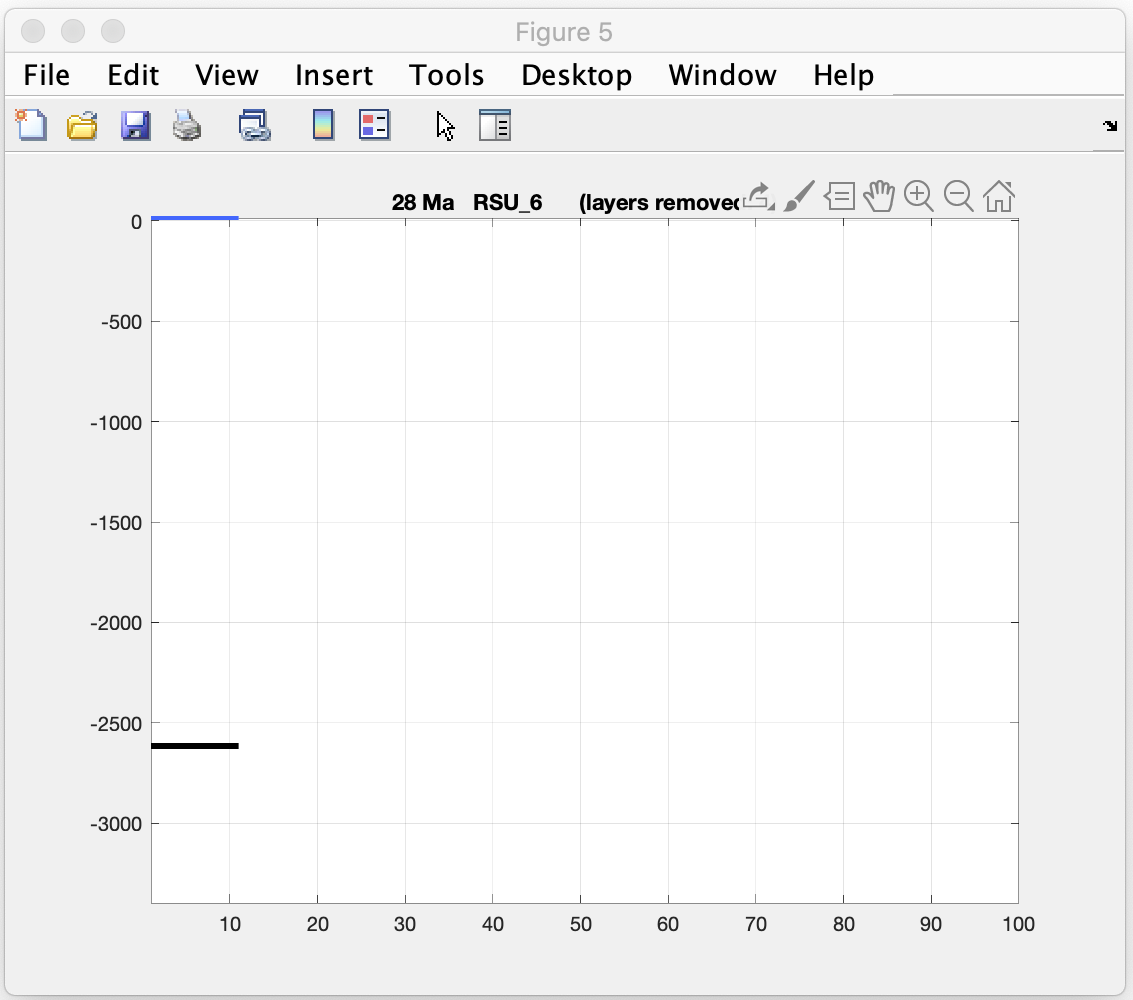
\includegraphics[scale=0.35]{Figures/1D/H02.png}
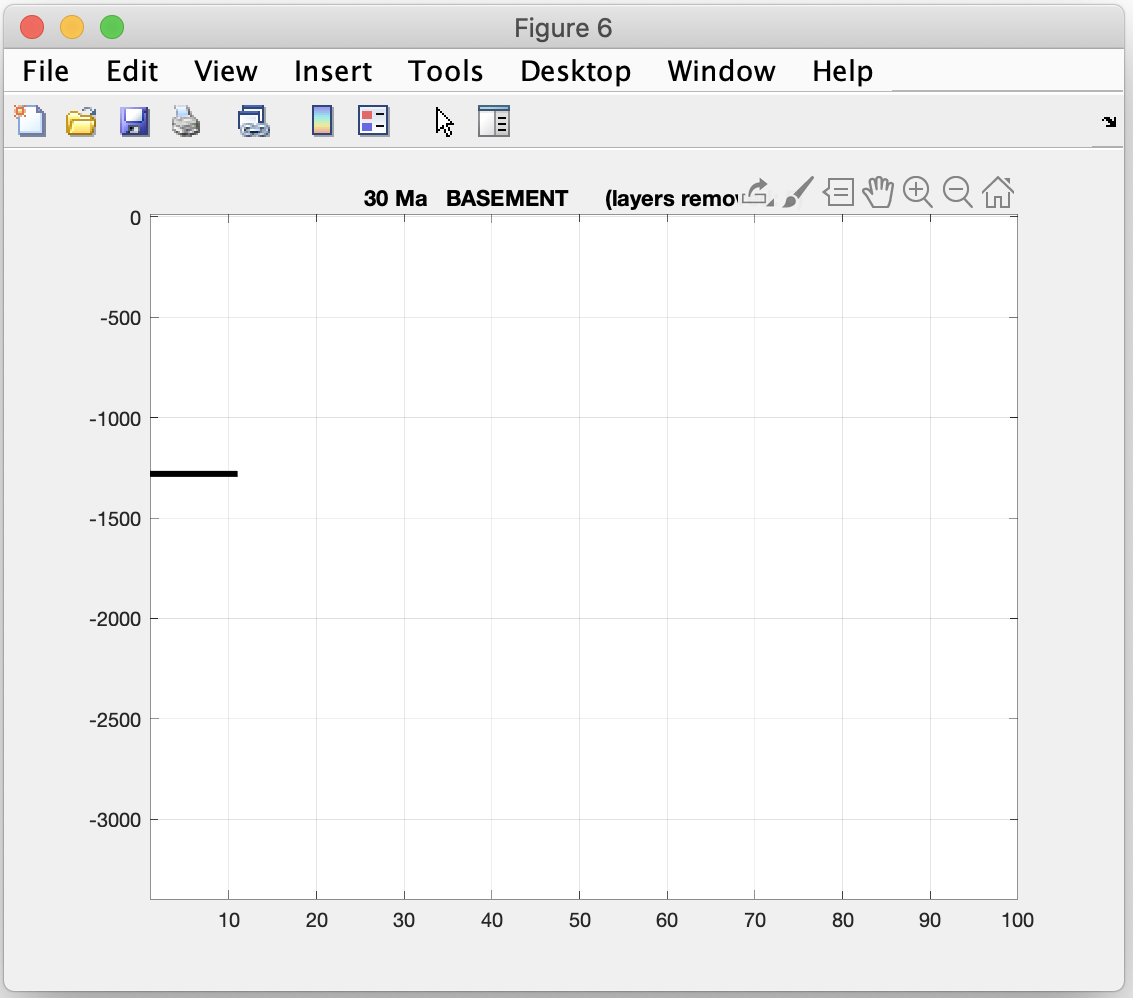
\includegraphics[scale=0.35]{Figures/1D/H01.png}\\
\end{figure}


\clearpage
\newpage
\subsection*{5- Save outputs}

Finally the user can save the outputs in ASCII files by selecting the variable to be saved:

\begin{figure}[!h]
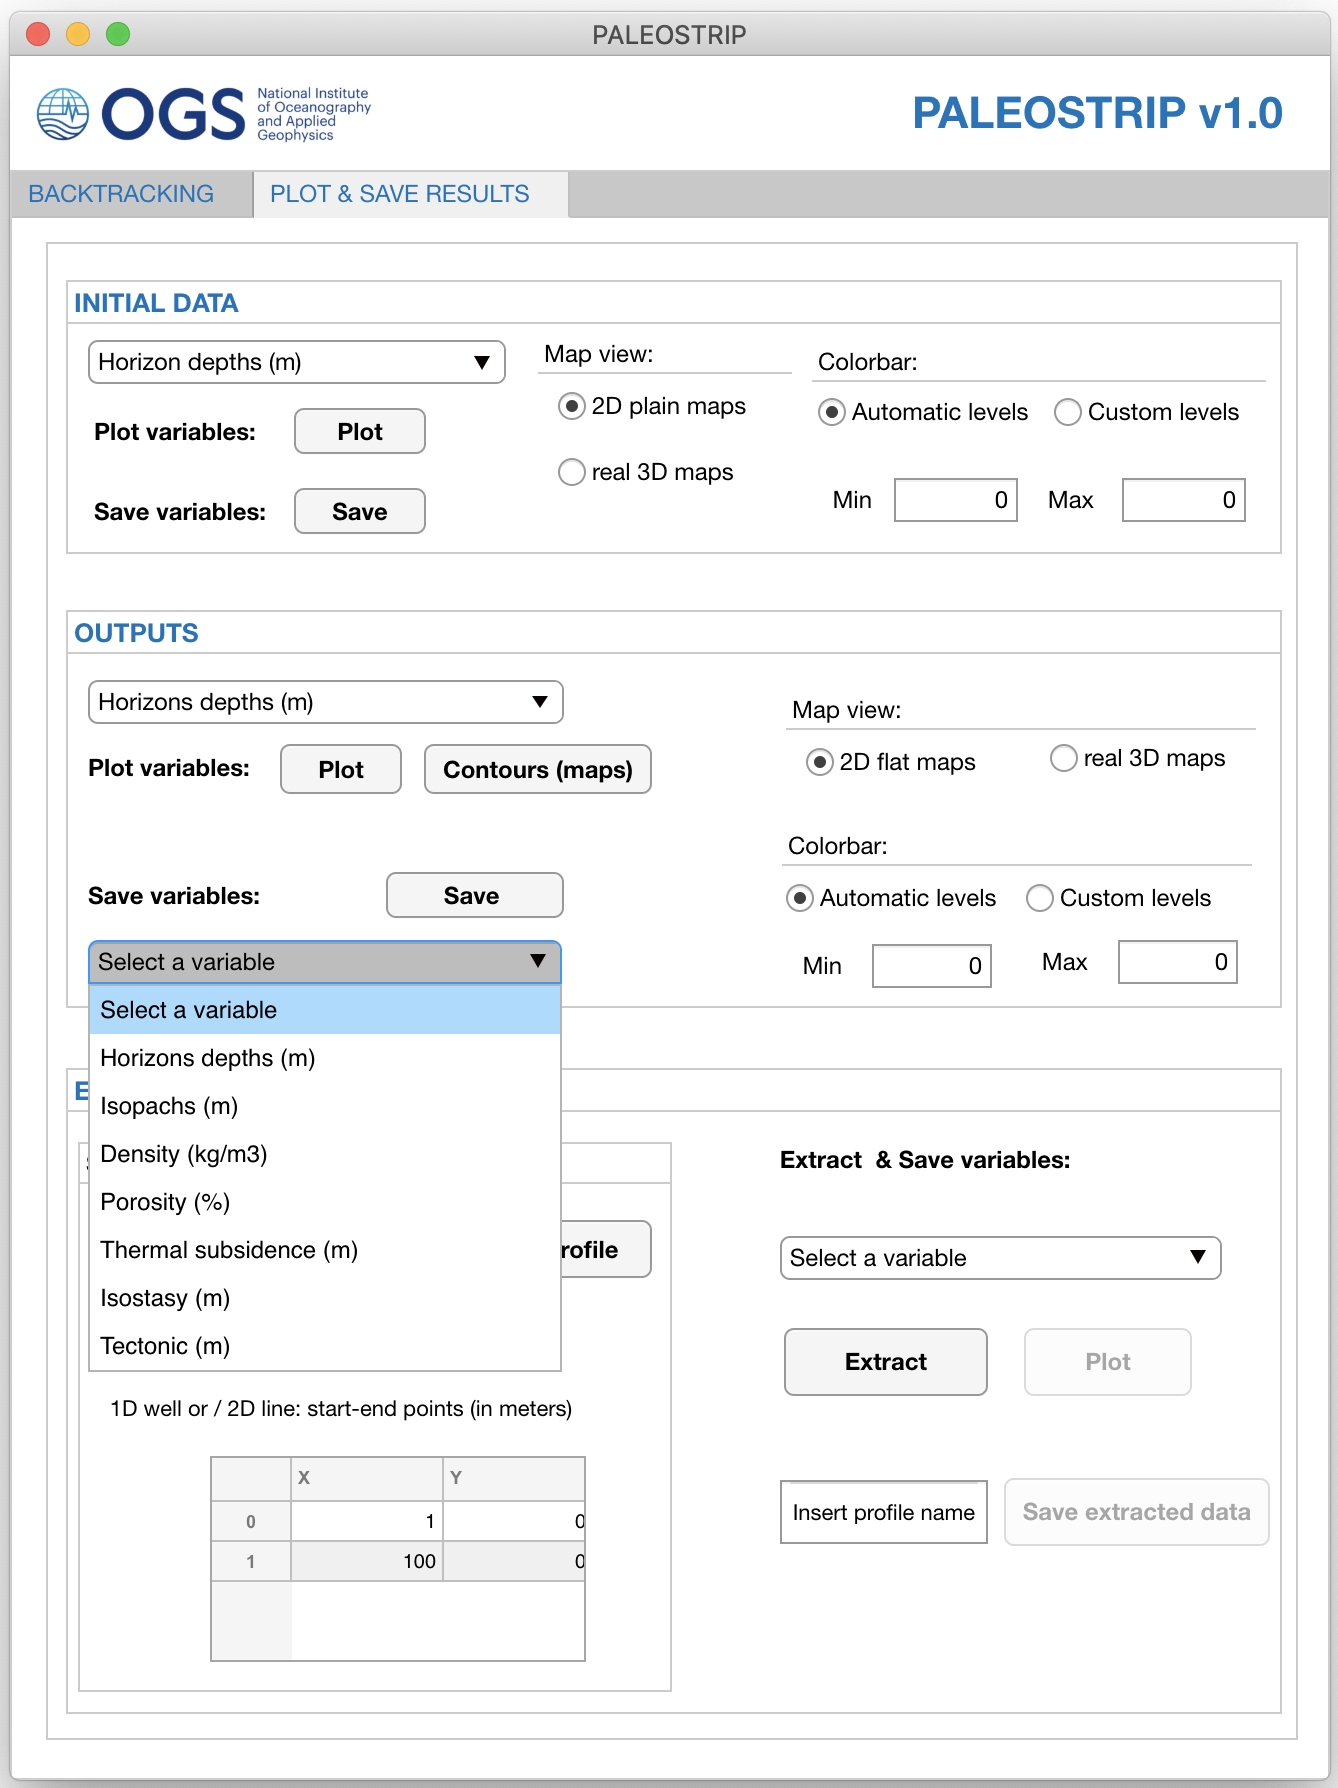
\includegraphics[scale=0.35]{Figures/1D/Save_outputs.png}
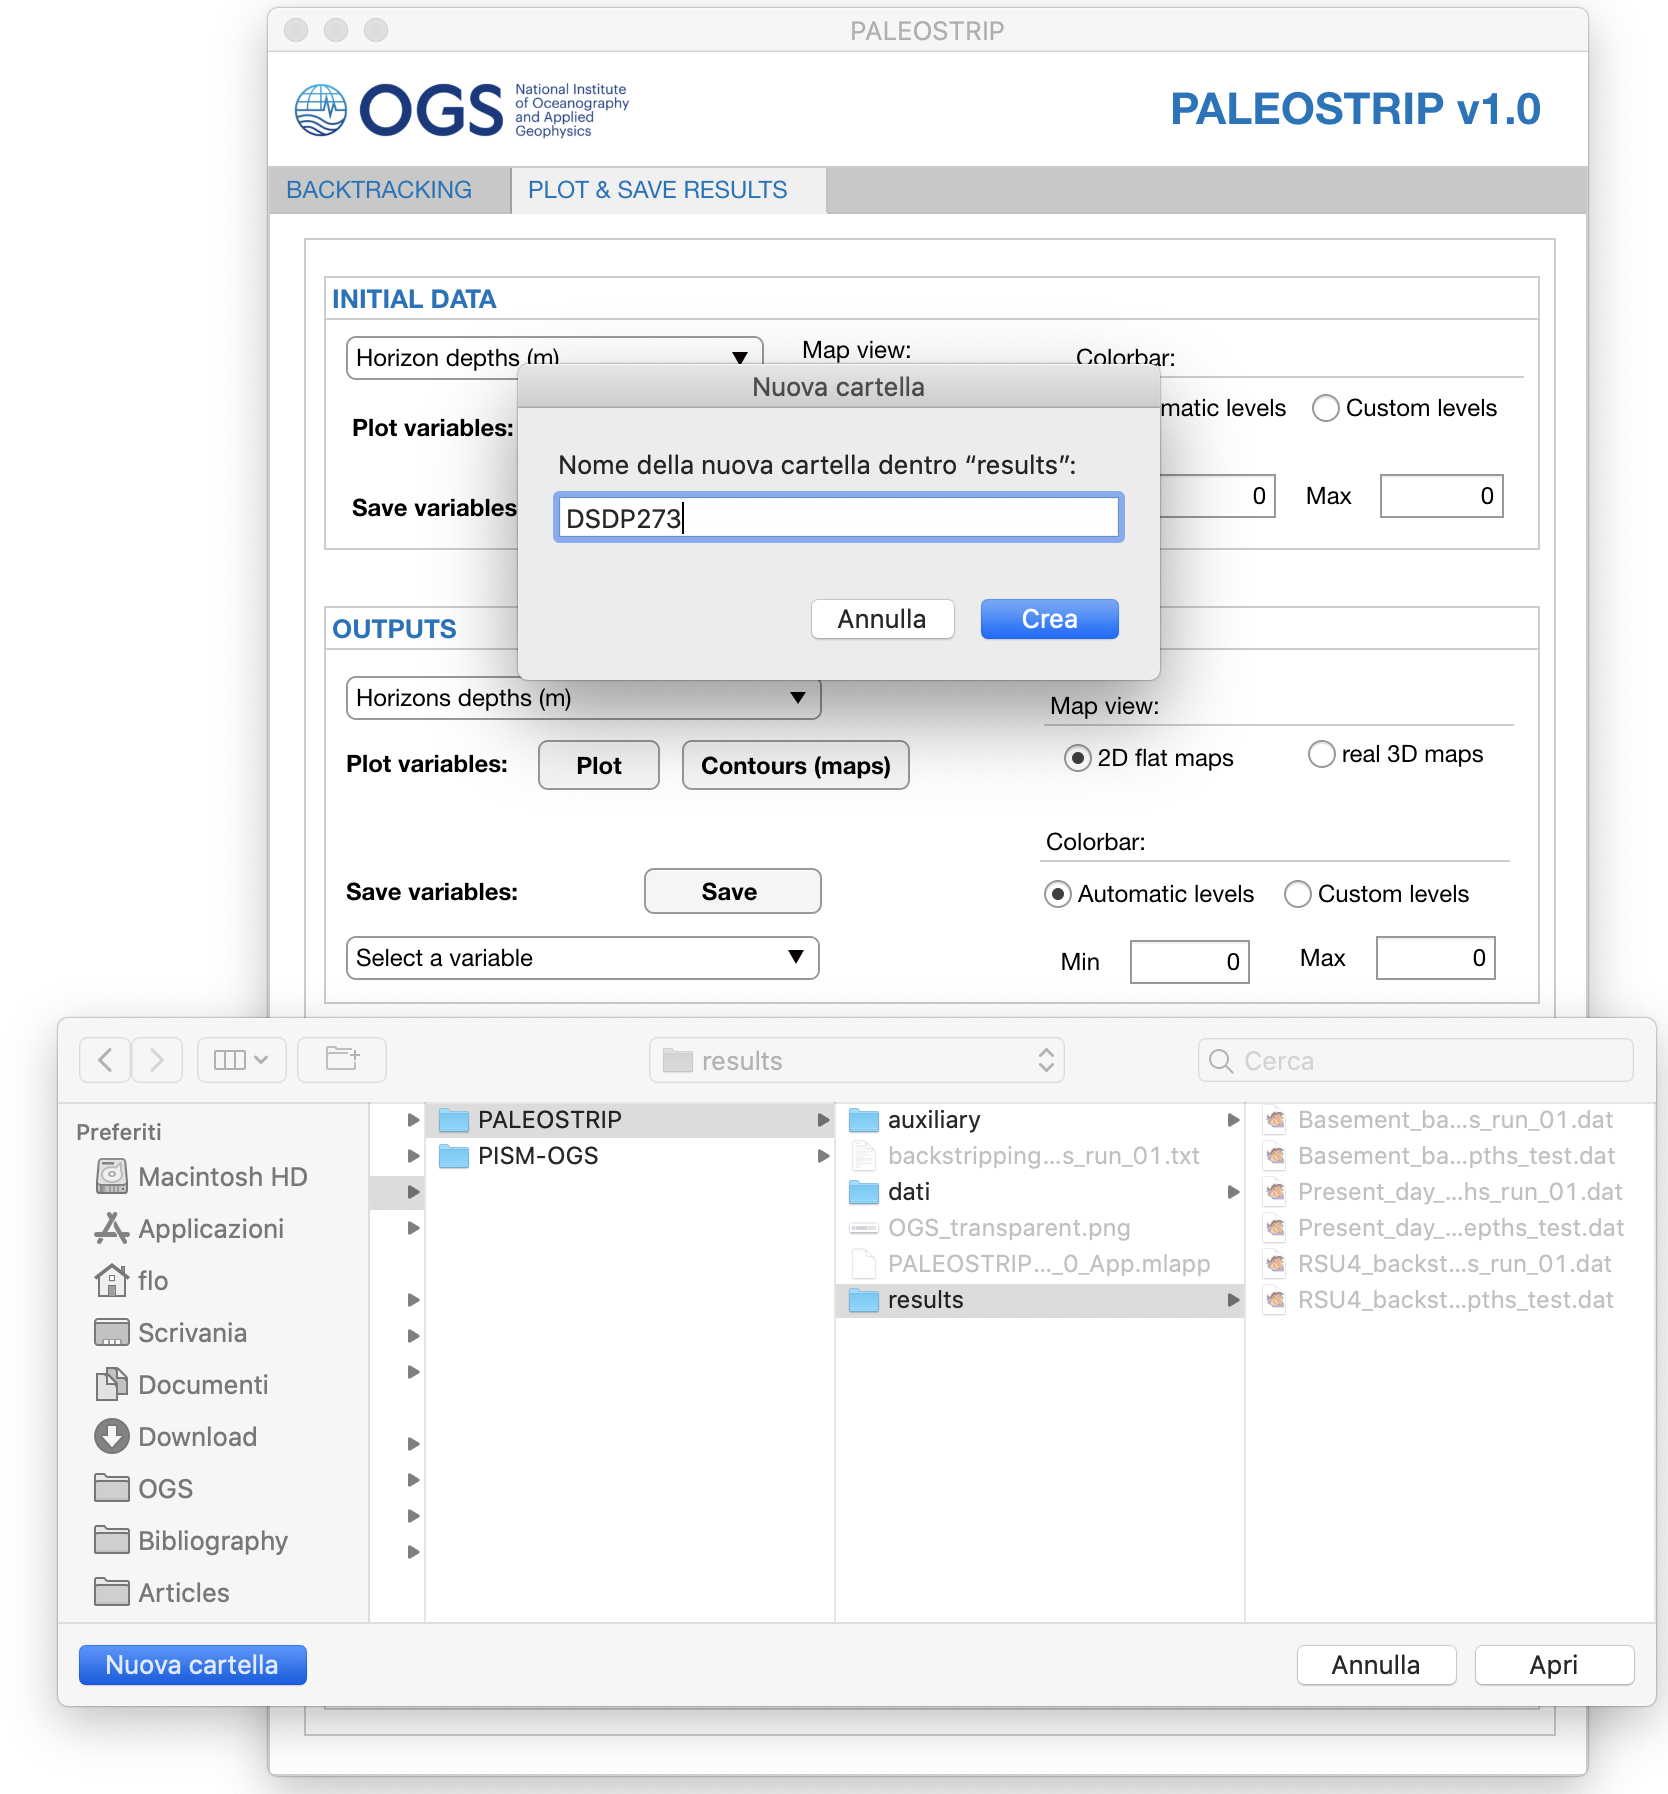
\includegraphics[scale=0.35]{Figures/1D/Save_outputs_dir.png}

\end{figure}

\begin{figure}[!h]
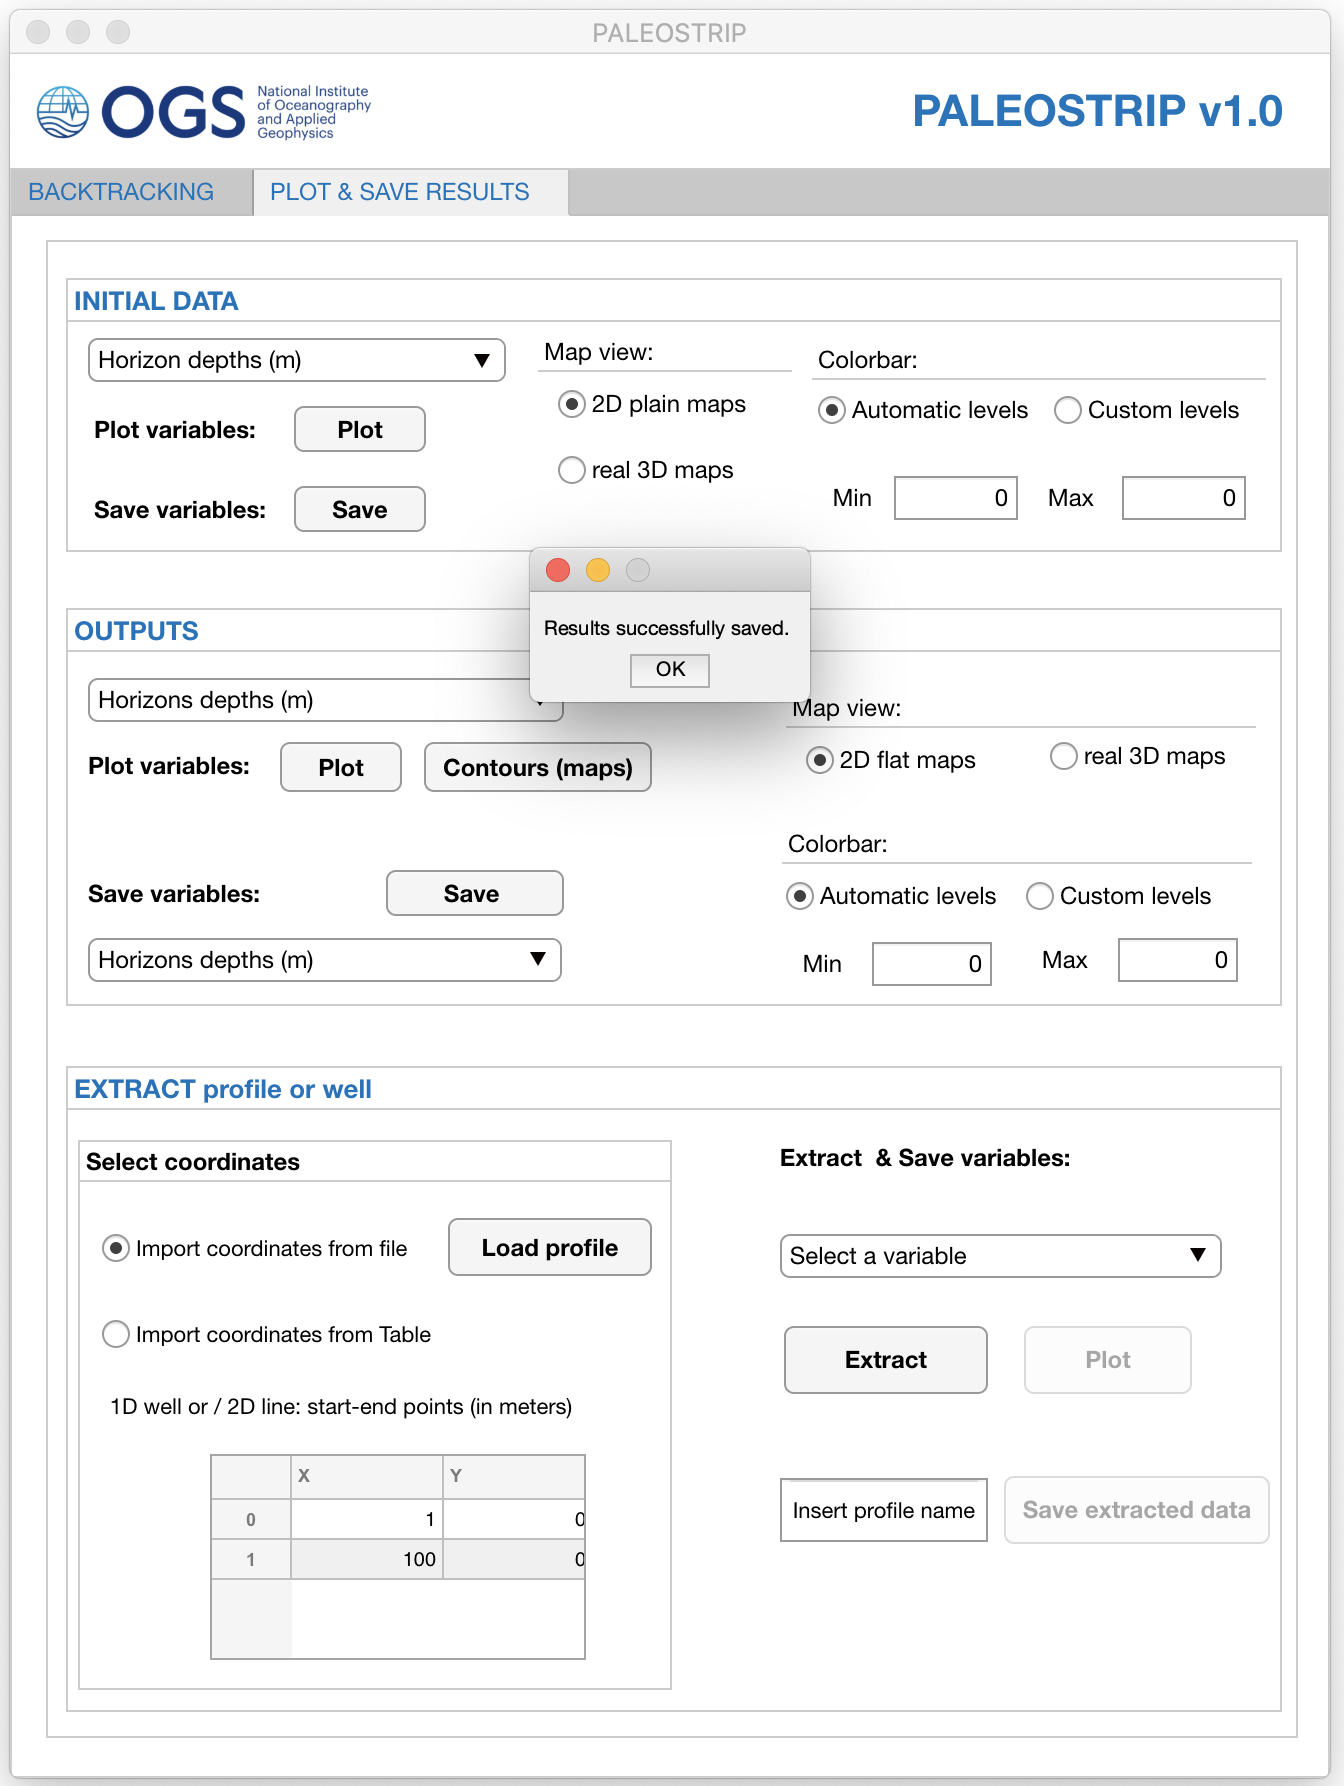
\includegraphics[scale=0.35]{Figures/1D/Results_successfully_saved.png}
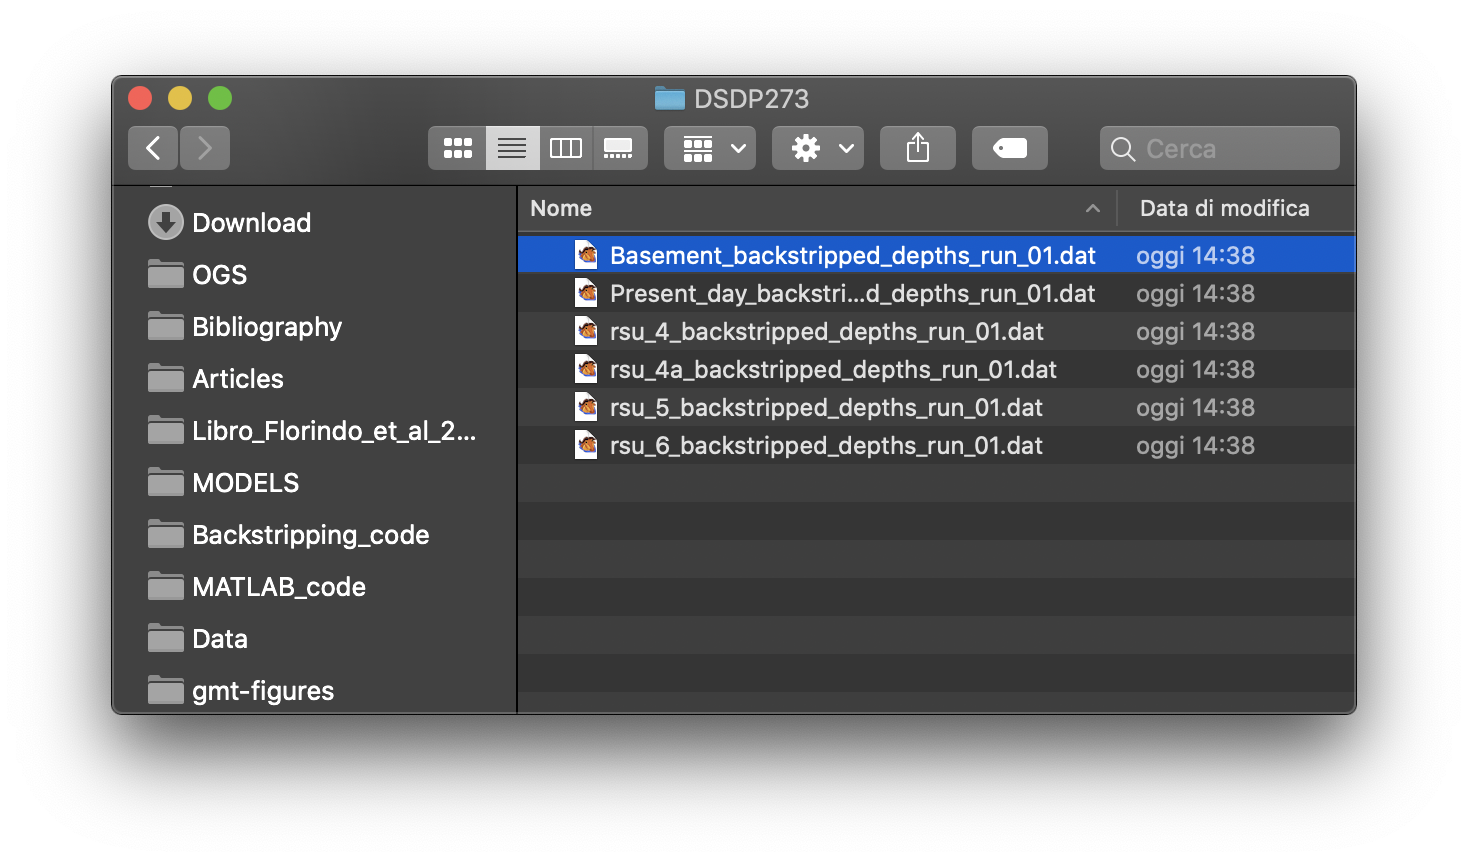
\includegraphics[scale=0.35]{Figures/1D/Saved_output_files.png}
\end{figure}


\clearpage
\newpage

\section{2D transect}

In the following sub-sections, we only show the steps or options that differ form the 1D case. If some steps are not shown, please refer to the previous example about 1D well.

\subsection*{1- Import data}

\begin{figure}[!h]
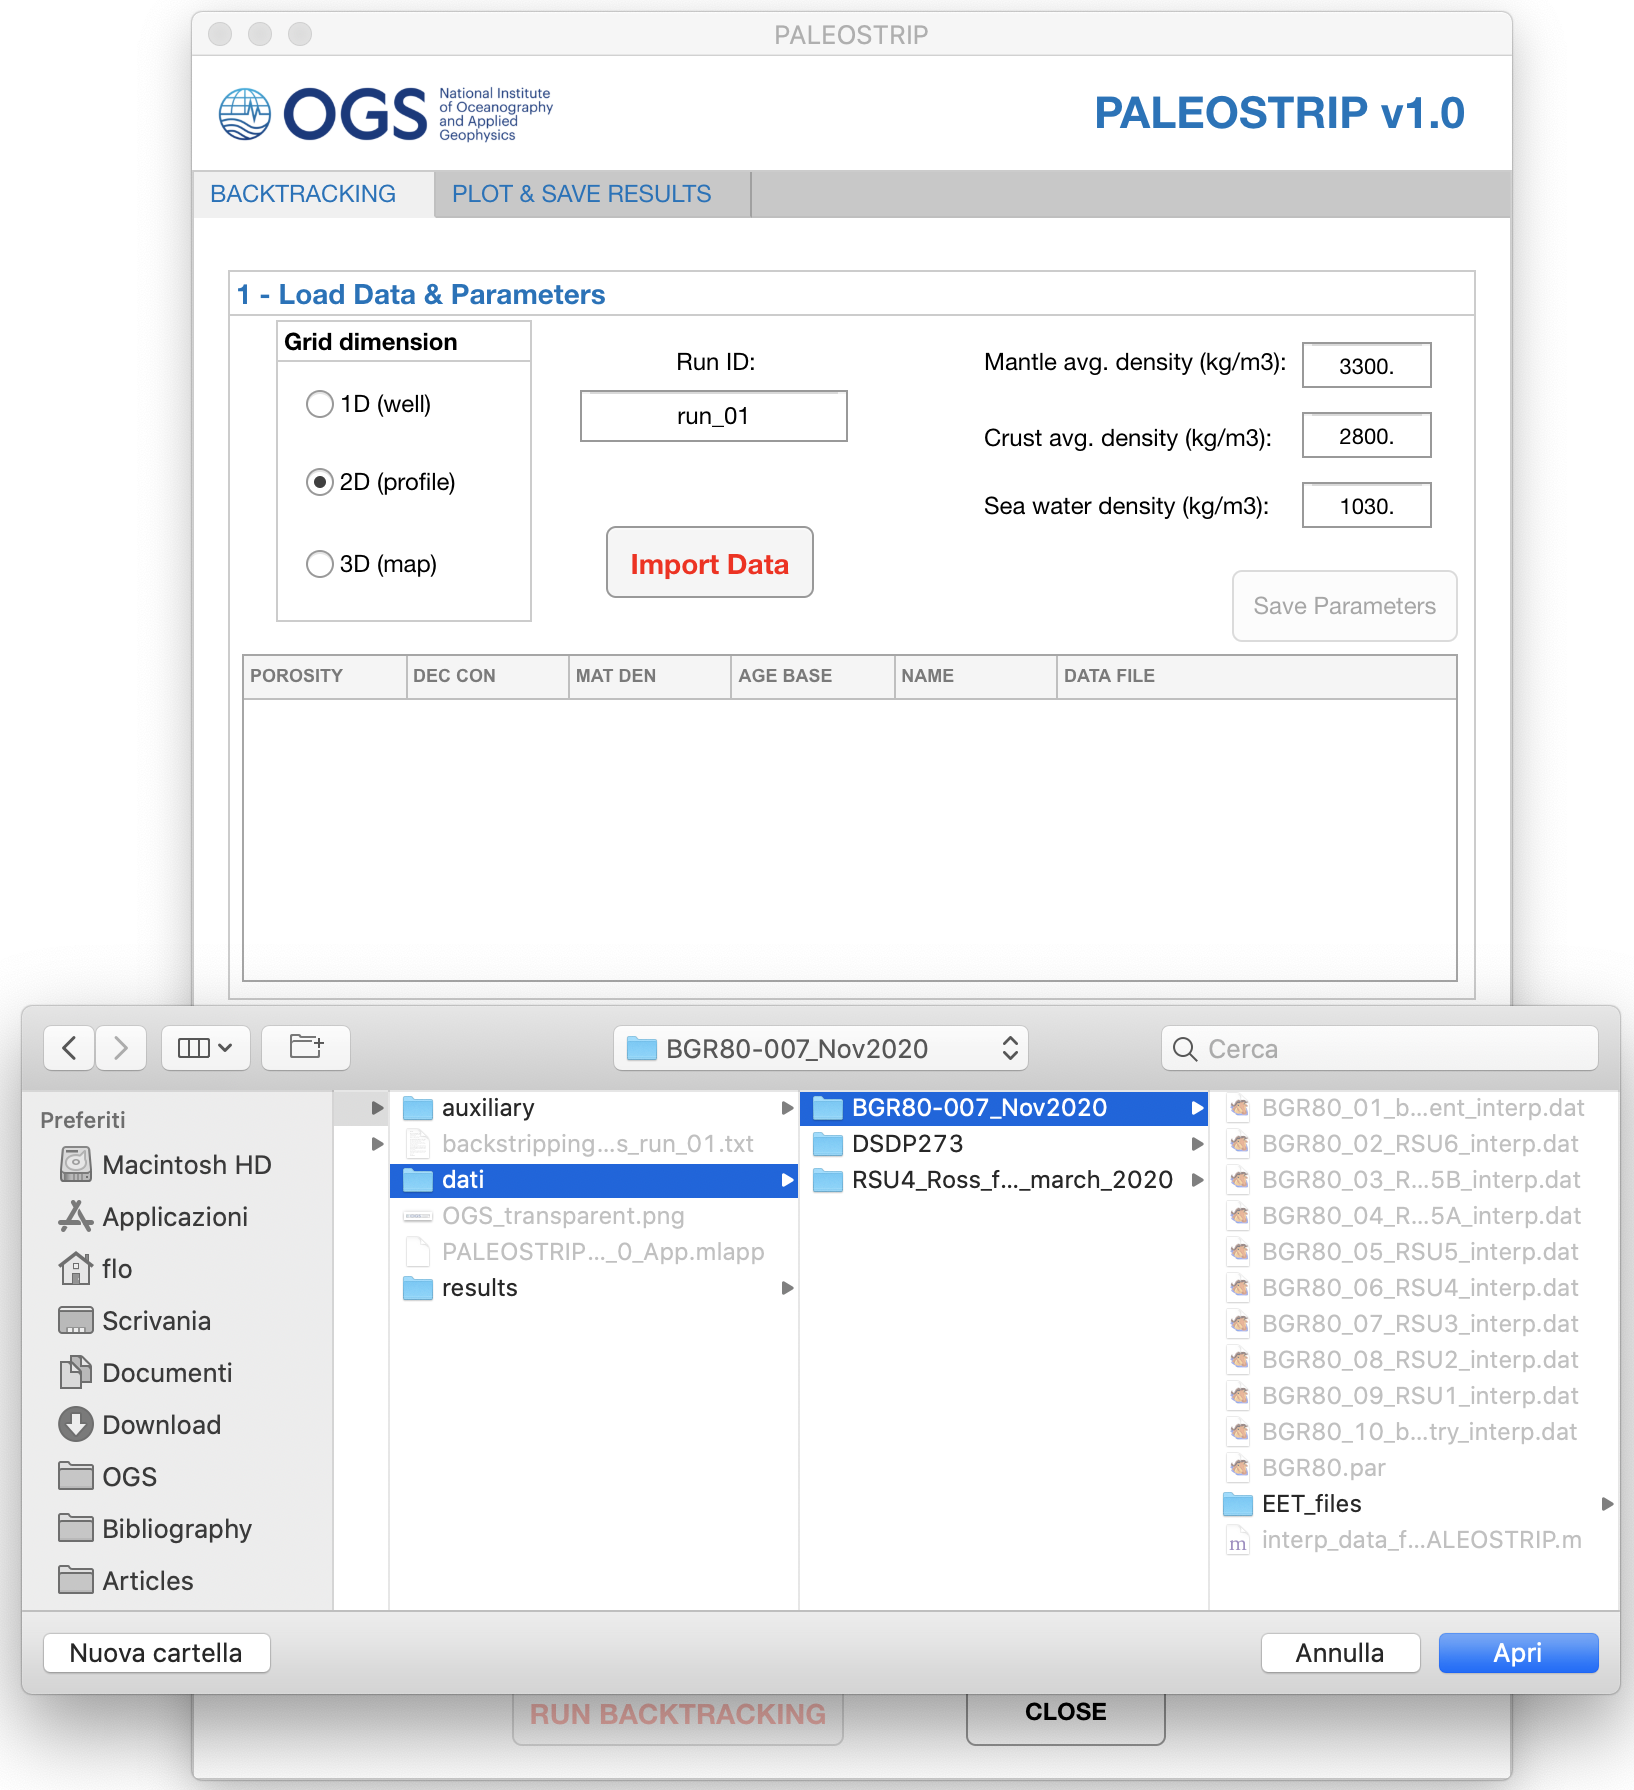
\includegraphics[scale=0.3]{Figures/2D/Input_data.png}
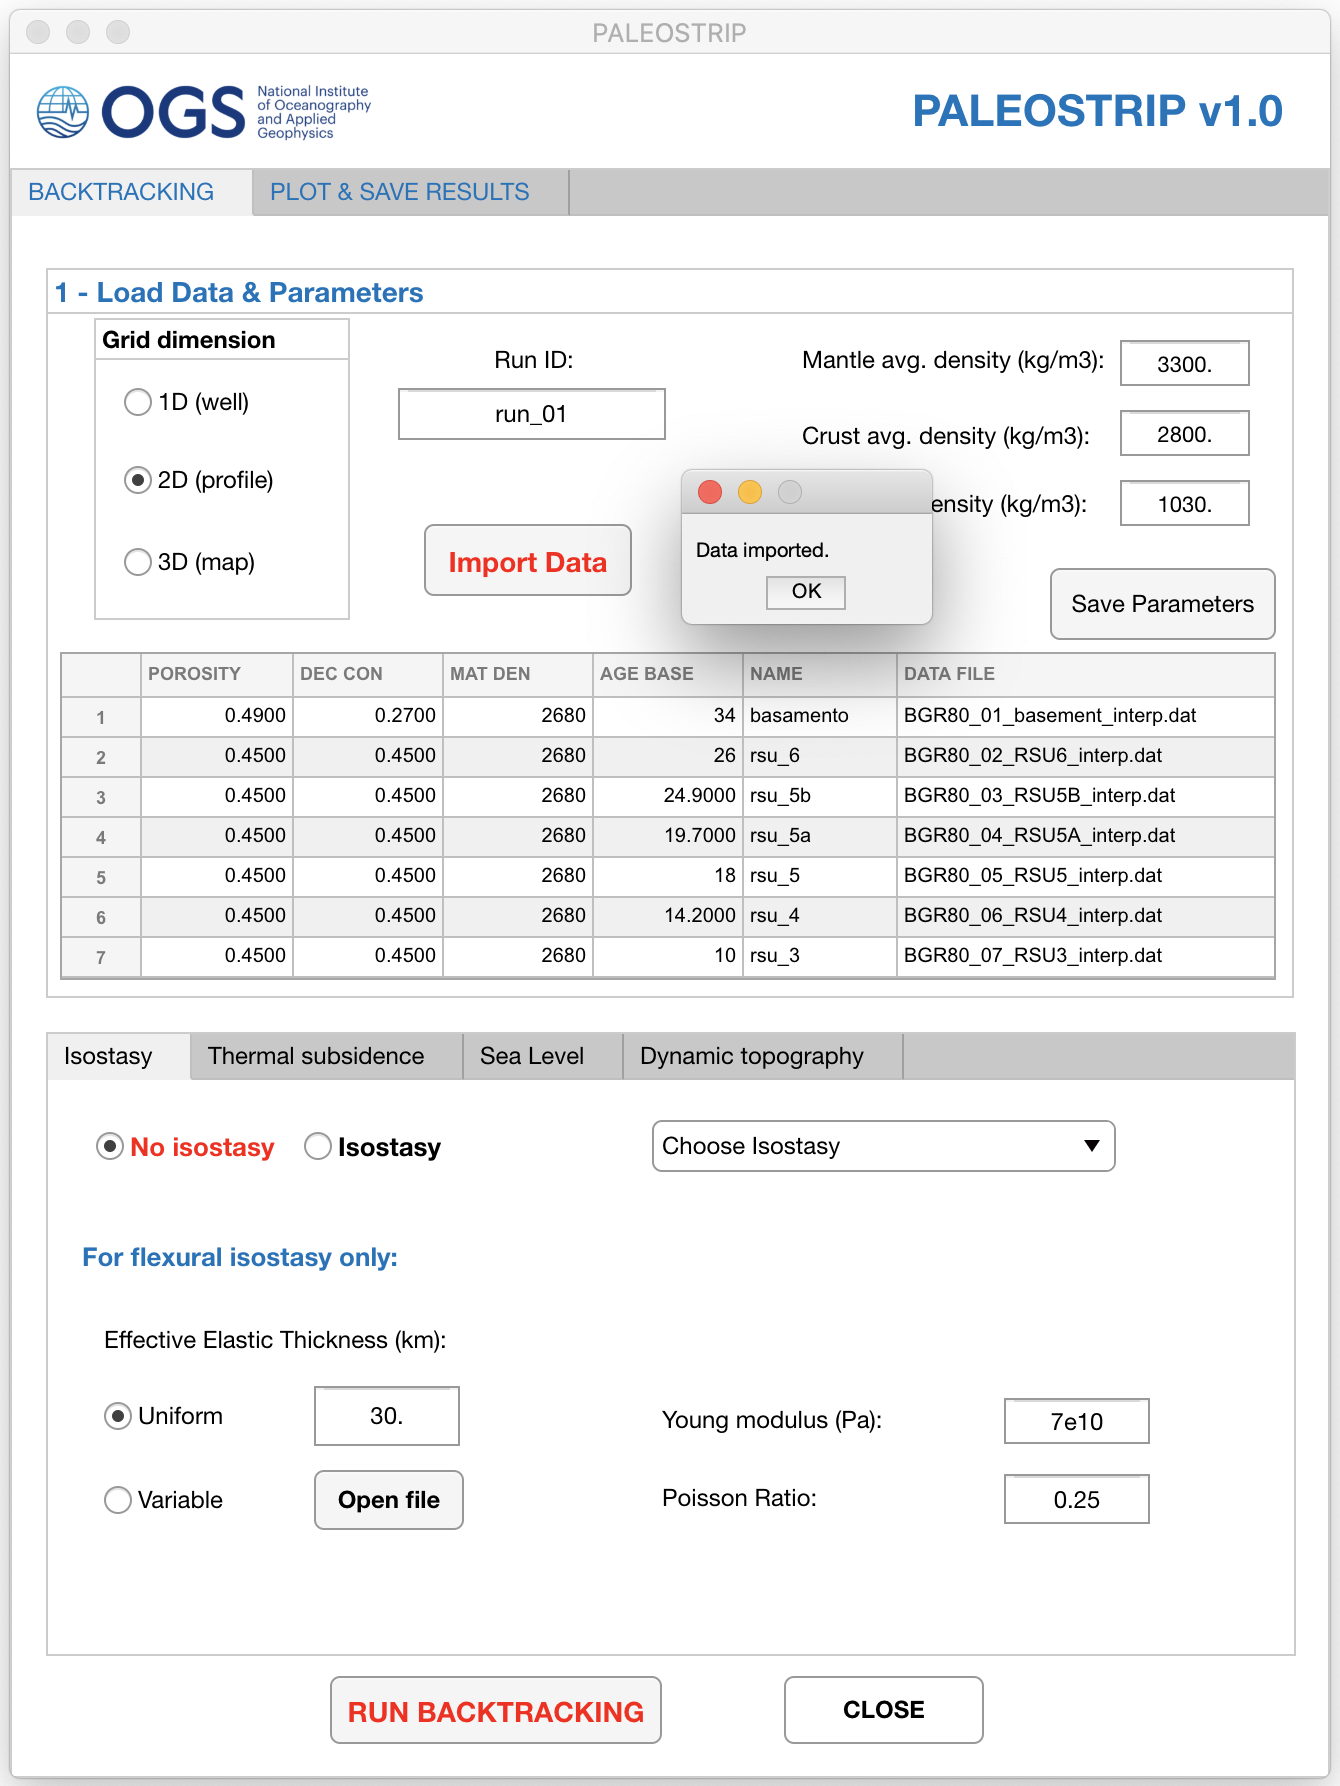
\includegraphics[scale=0.3]{Figures/2D/Imported_data_OK.png}
\end{figure}

\subsection*{2- Select physical parameters and corrections}

Here, we use flexural isostasy with fixed effective elastic thickness set to 30 km. Options for thermal subsidence, sea level and dynamic topography are identical to the 1D well example.

\begin{figure}[!h]
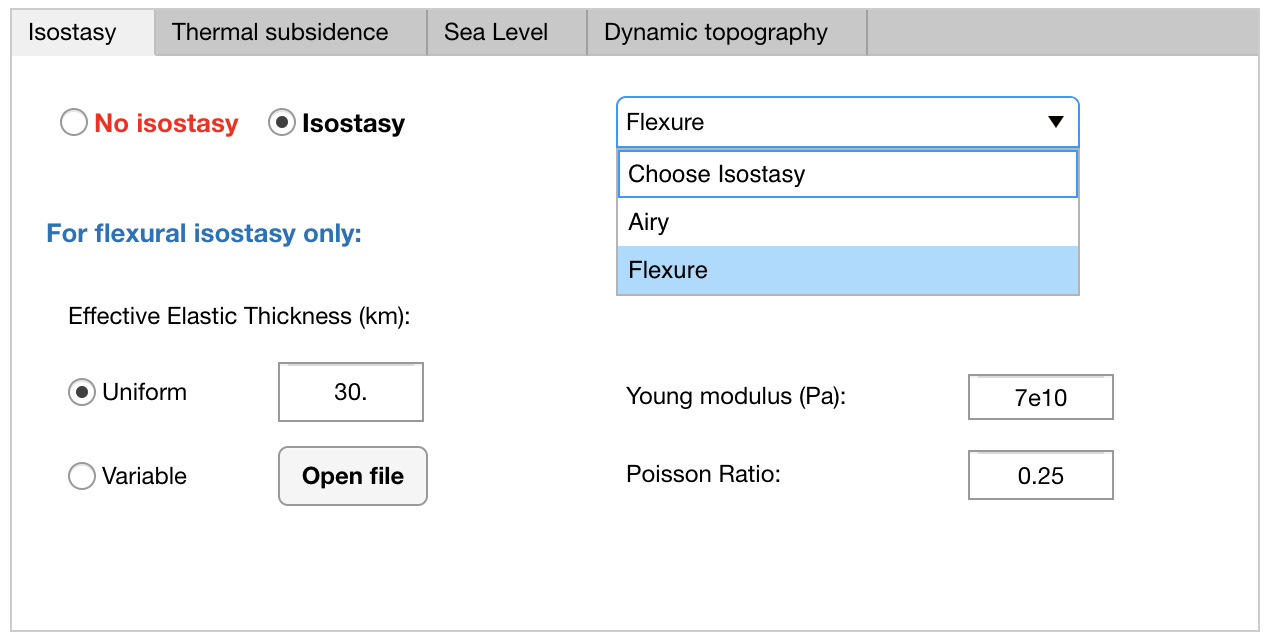
\includegraphics[scale=0.4]{Figures/2D/Isostasy_flex_Te30km.png}
\end{figure}


\clearpage
\newpage
\subsection*{3- Run Backtracking}

The procedure is identical to that shown for 1D well example above.


\subsection*{4- Plot outputs}

\begin{figure}[!h]
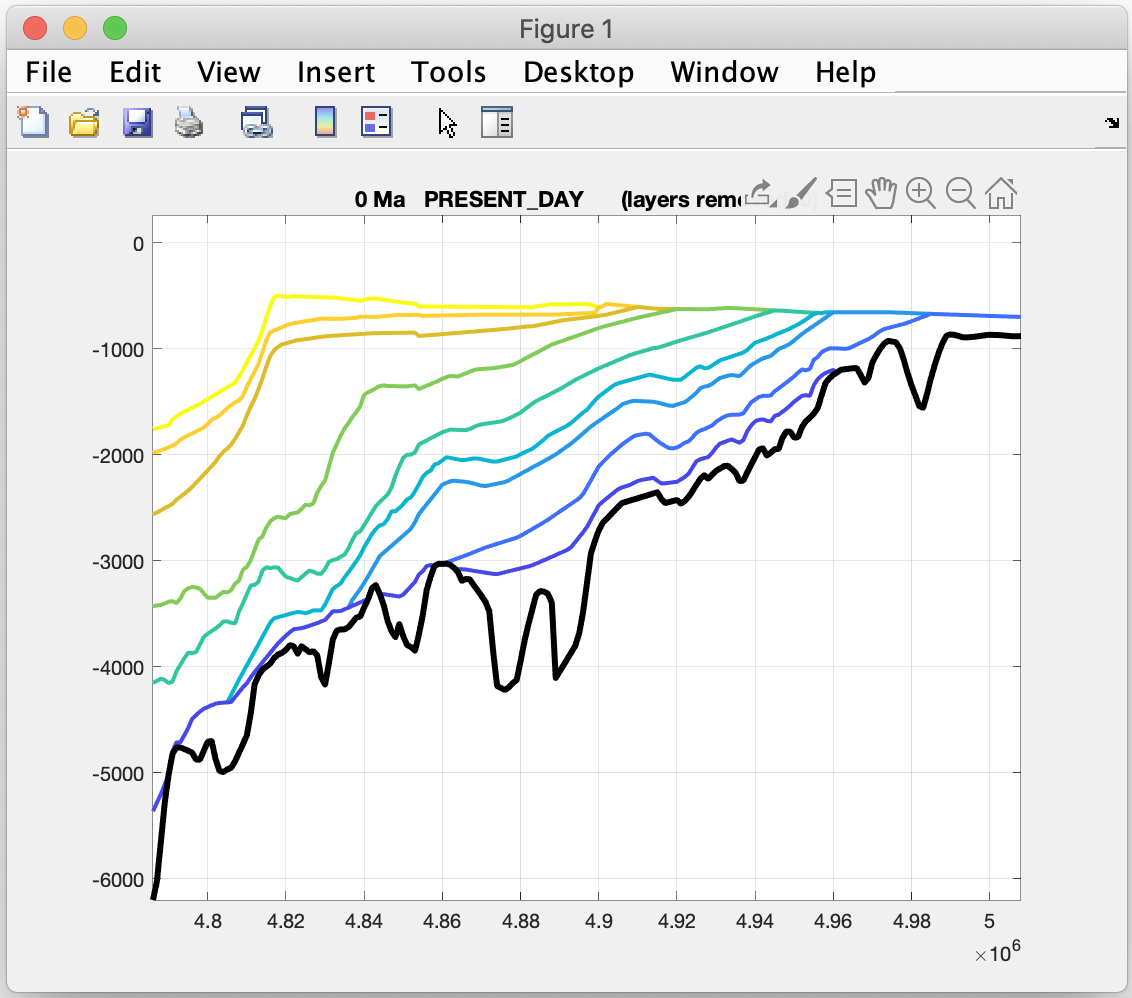
\includegraphics[scale=0.35]{Figures/2D/H10.png}
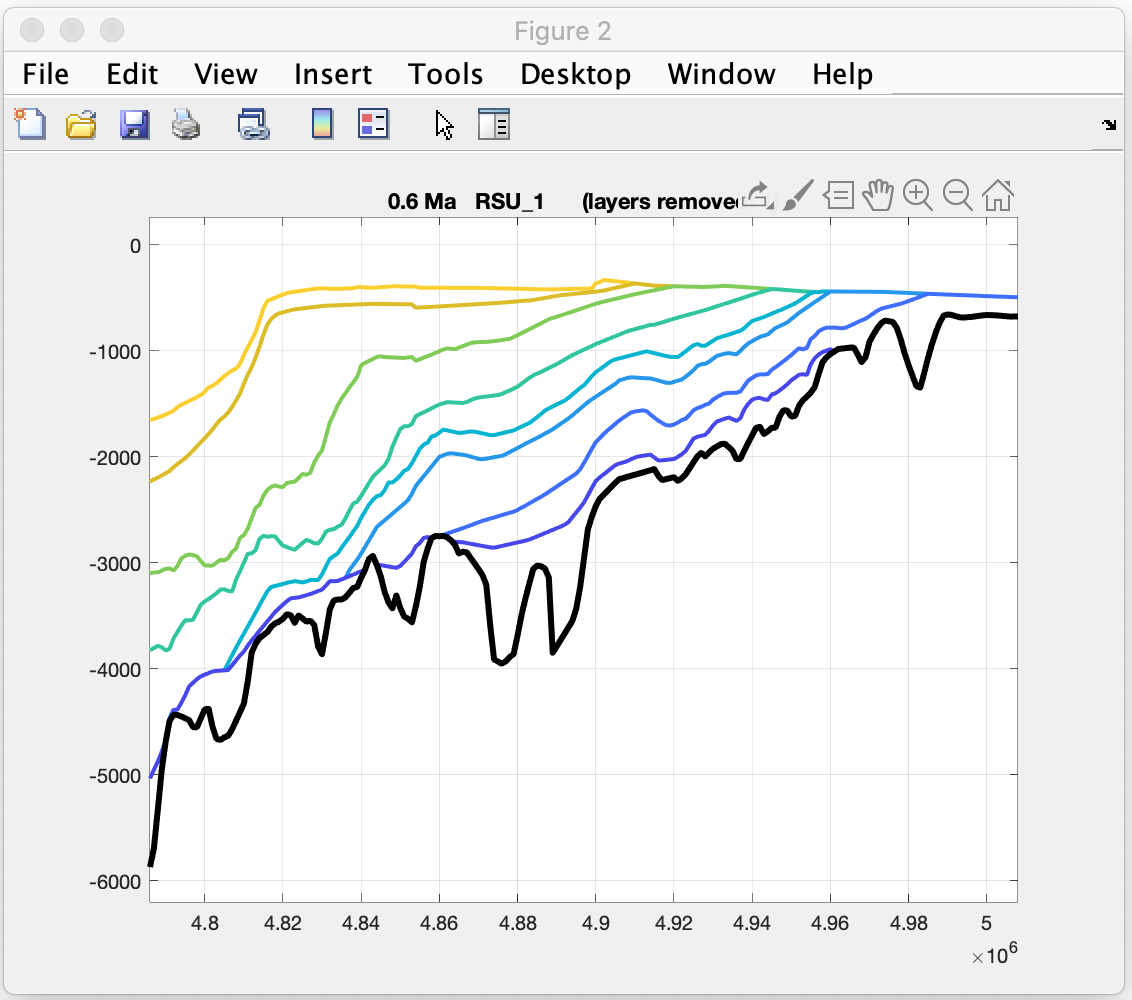
\includegraphics[scale=0.35]{Figures/2D/H09.png}\\
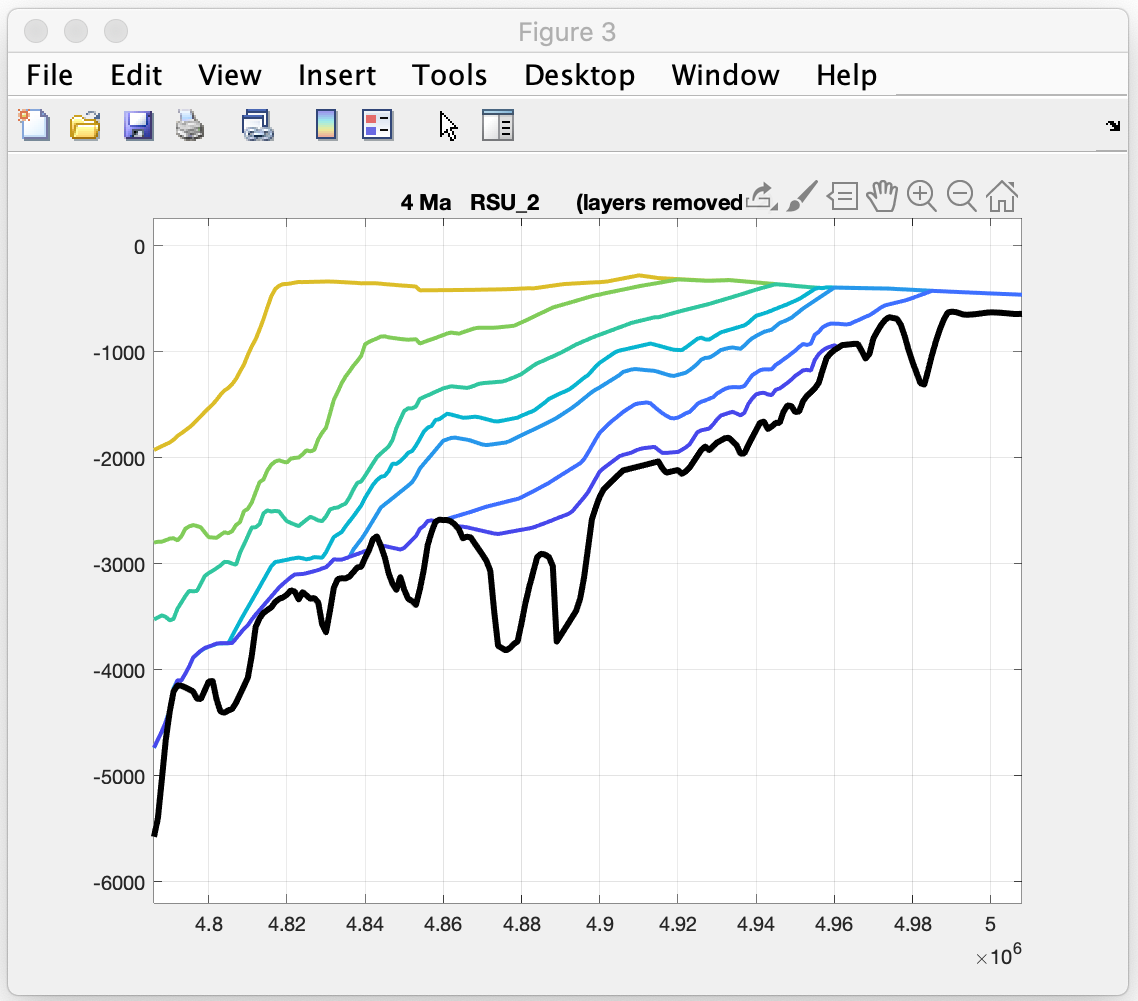
\includegraphics[scale=0.35]{Figures/2D/H08.png}
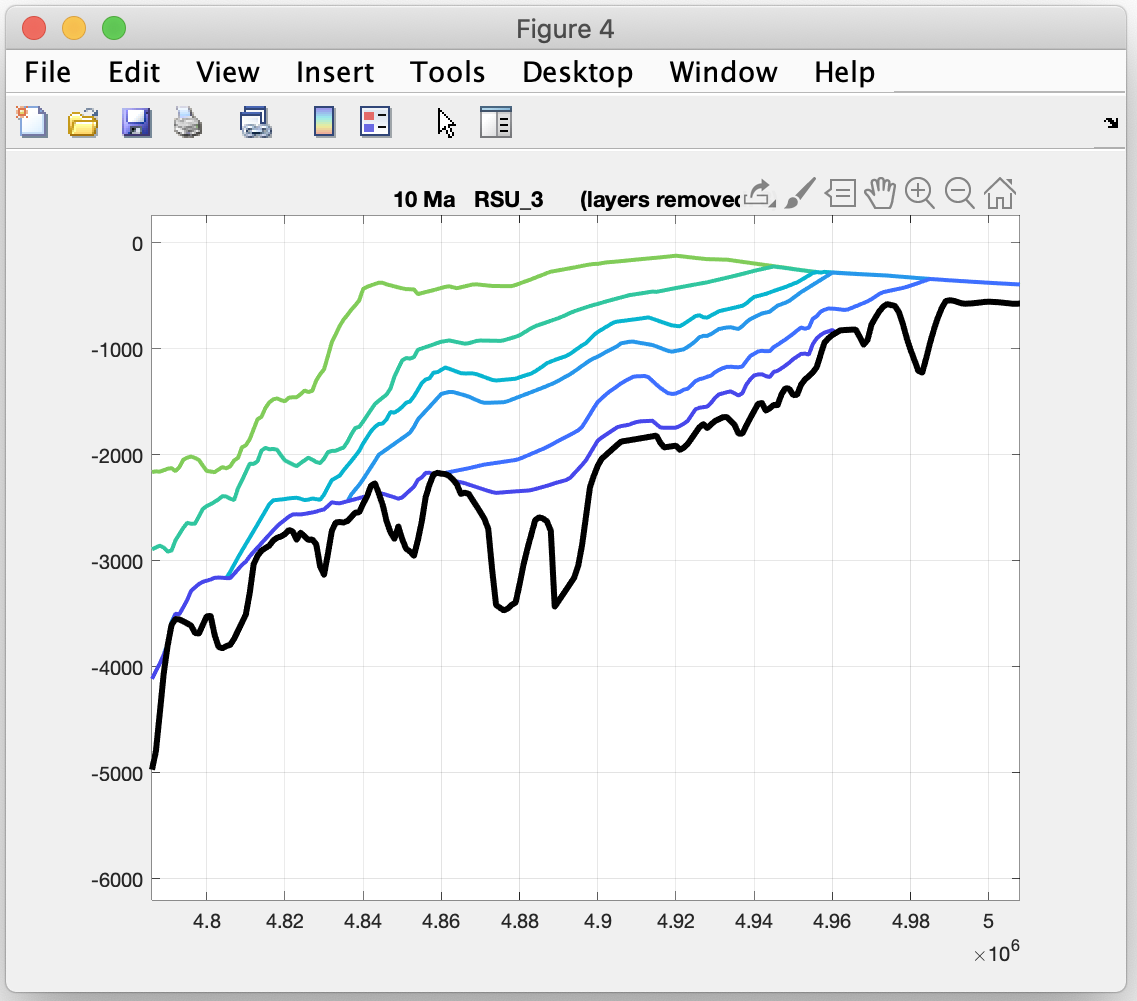
\includegraphics[scale=0.35]{Figures/2D/H07.png}\\
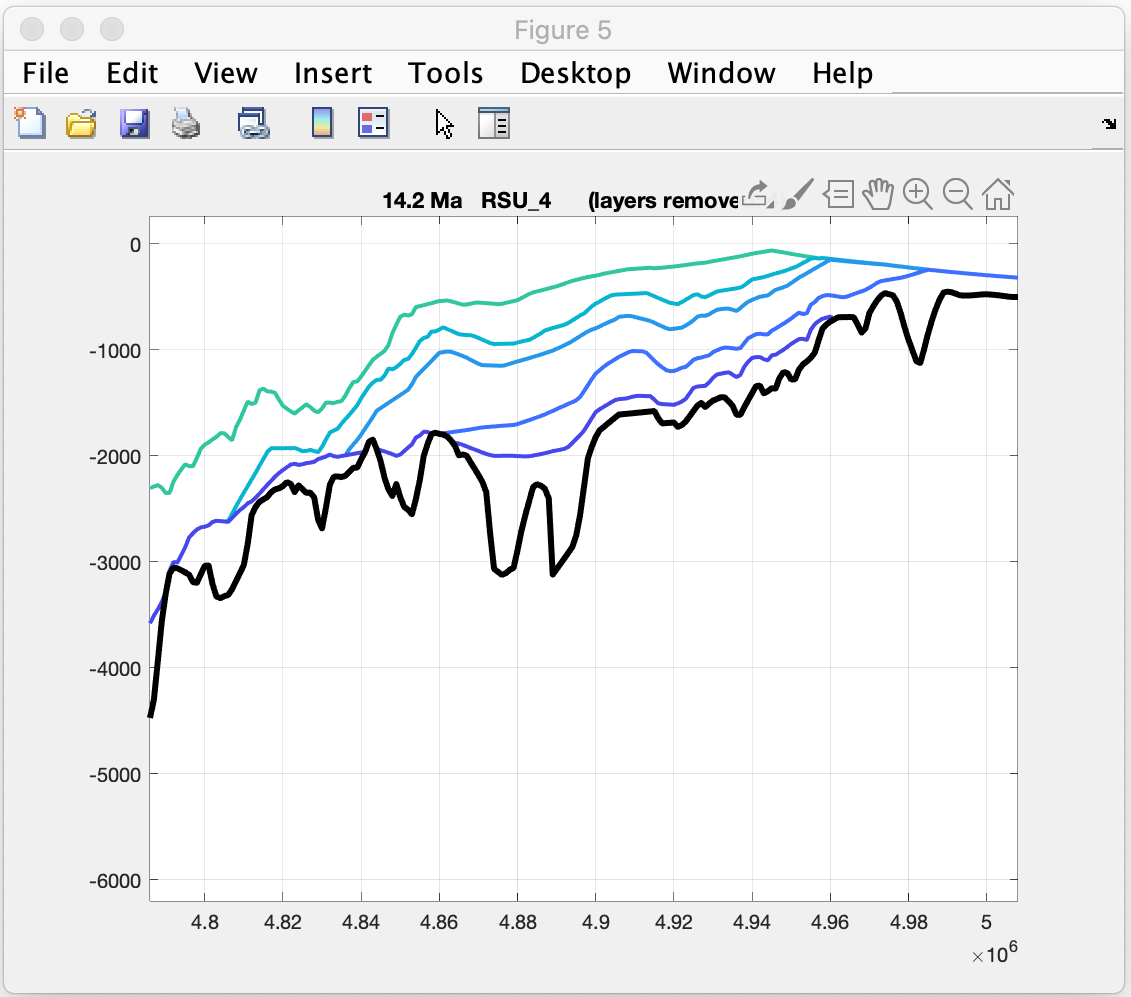
\includegraphics[scale=0.35]{Figures/2D/H06.png}
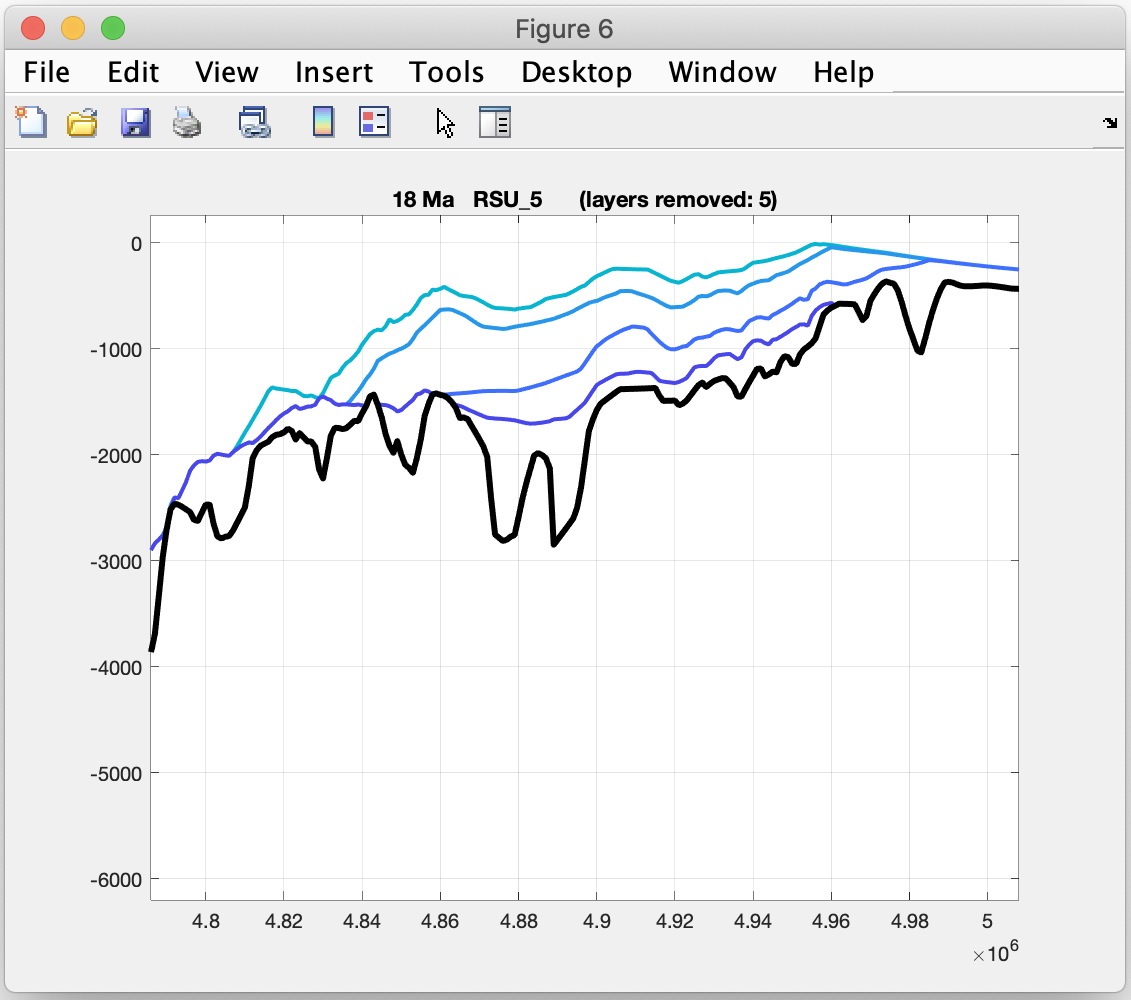
\includegraphics[scale=0.35]{Figures/2D/H05.png}\\
\end{figure}


\begin{figure}[!h]
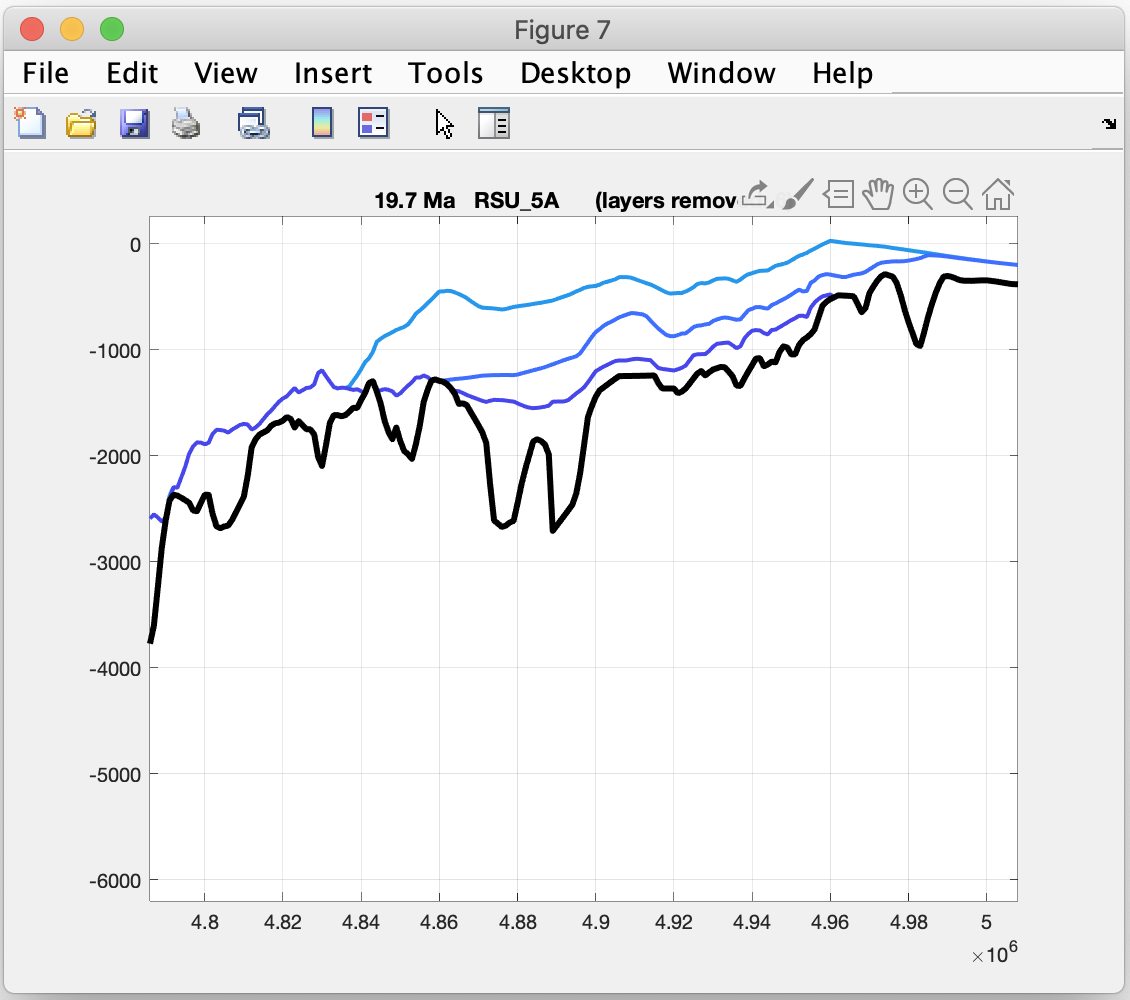
\includegraphics[scale=0.35]{Figures/2D/H04.png}
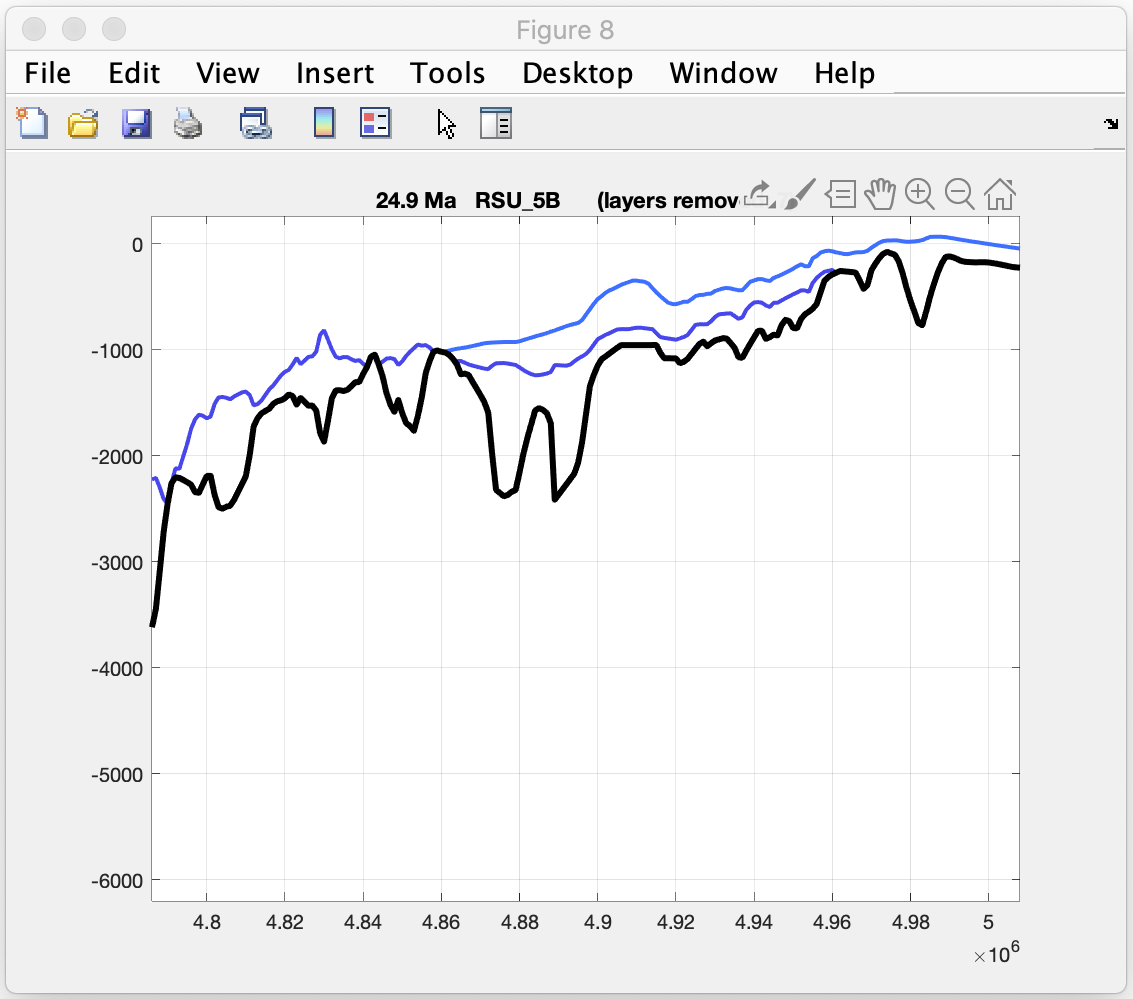
\includegraphics[scale=0.35]{Figures/2D/H03.png}\\
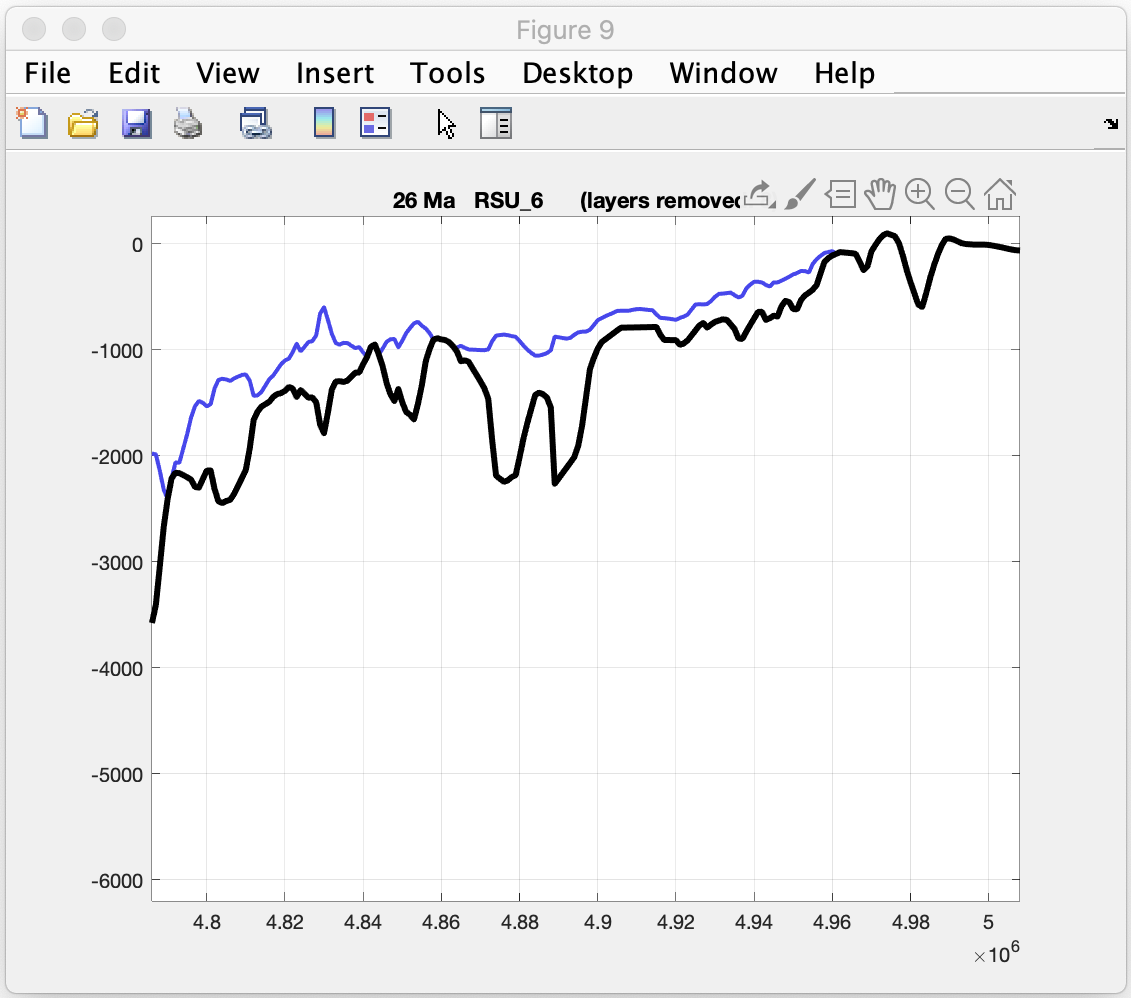
\includegraphics[scale=0.35]{Figures/2D/H02.png}
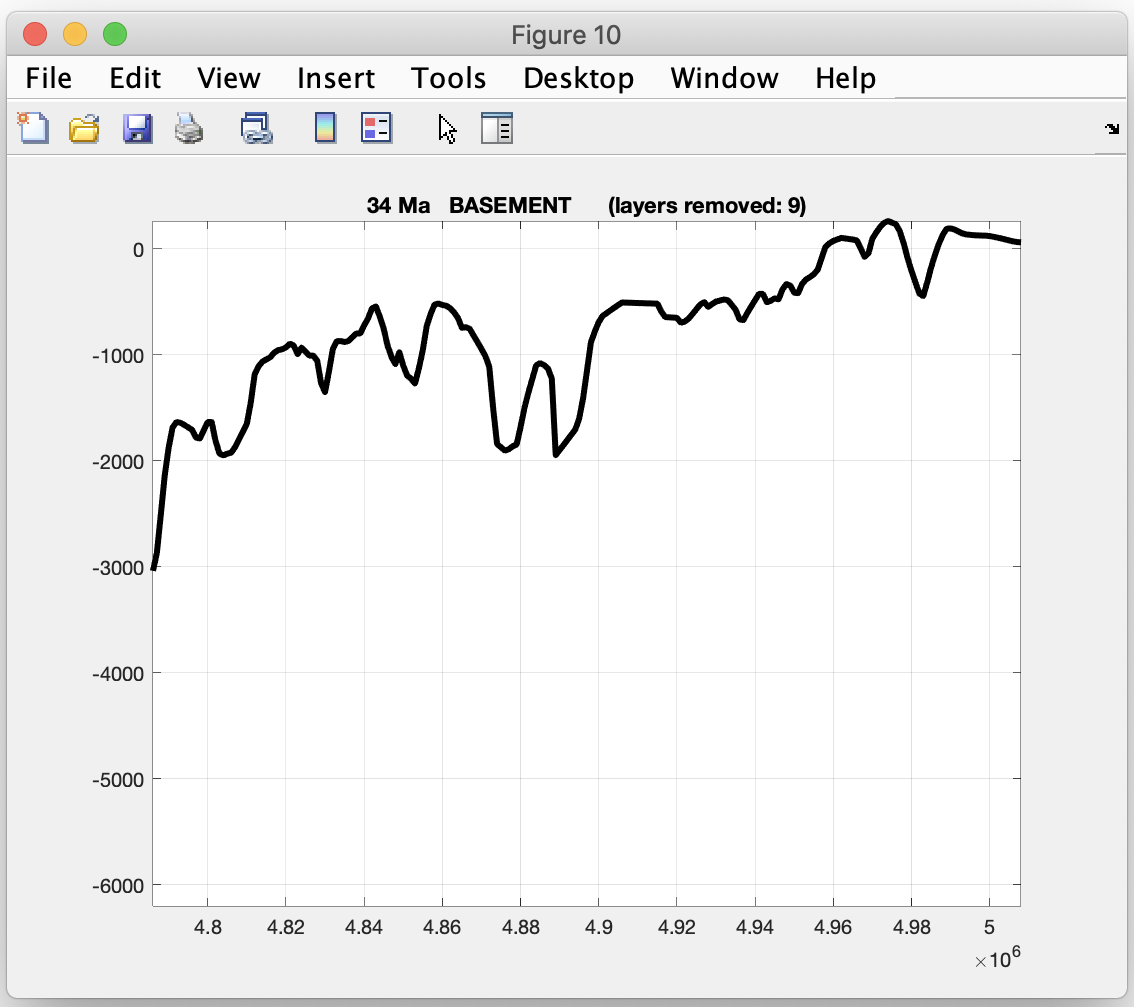
\includegraphics[scale=0.35]{Figures/2D/H01.png}\\
\end{figure}


\subsection*{5- Save outputs}

The procedure is identical to that shown for 1D well example above.



\clearpage
\newpage

\section{3D maps}

\subsection*{1- Import data}

\begin{figure}[!h]
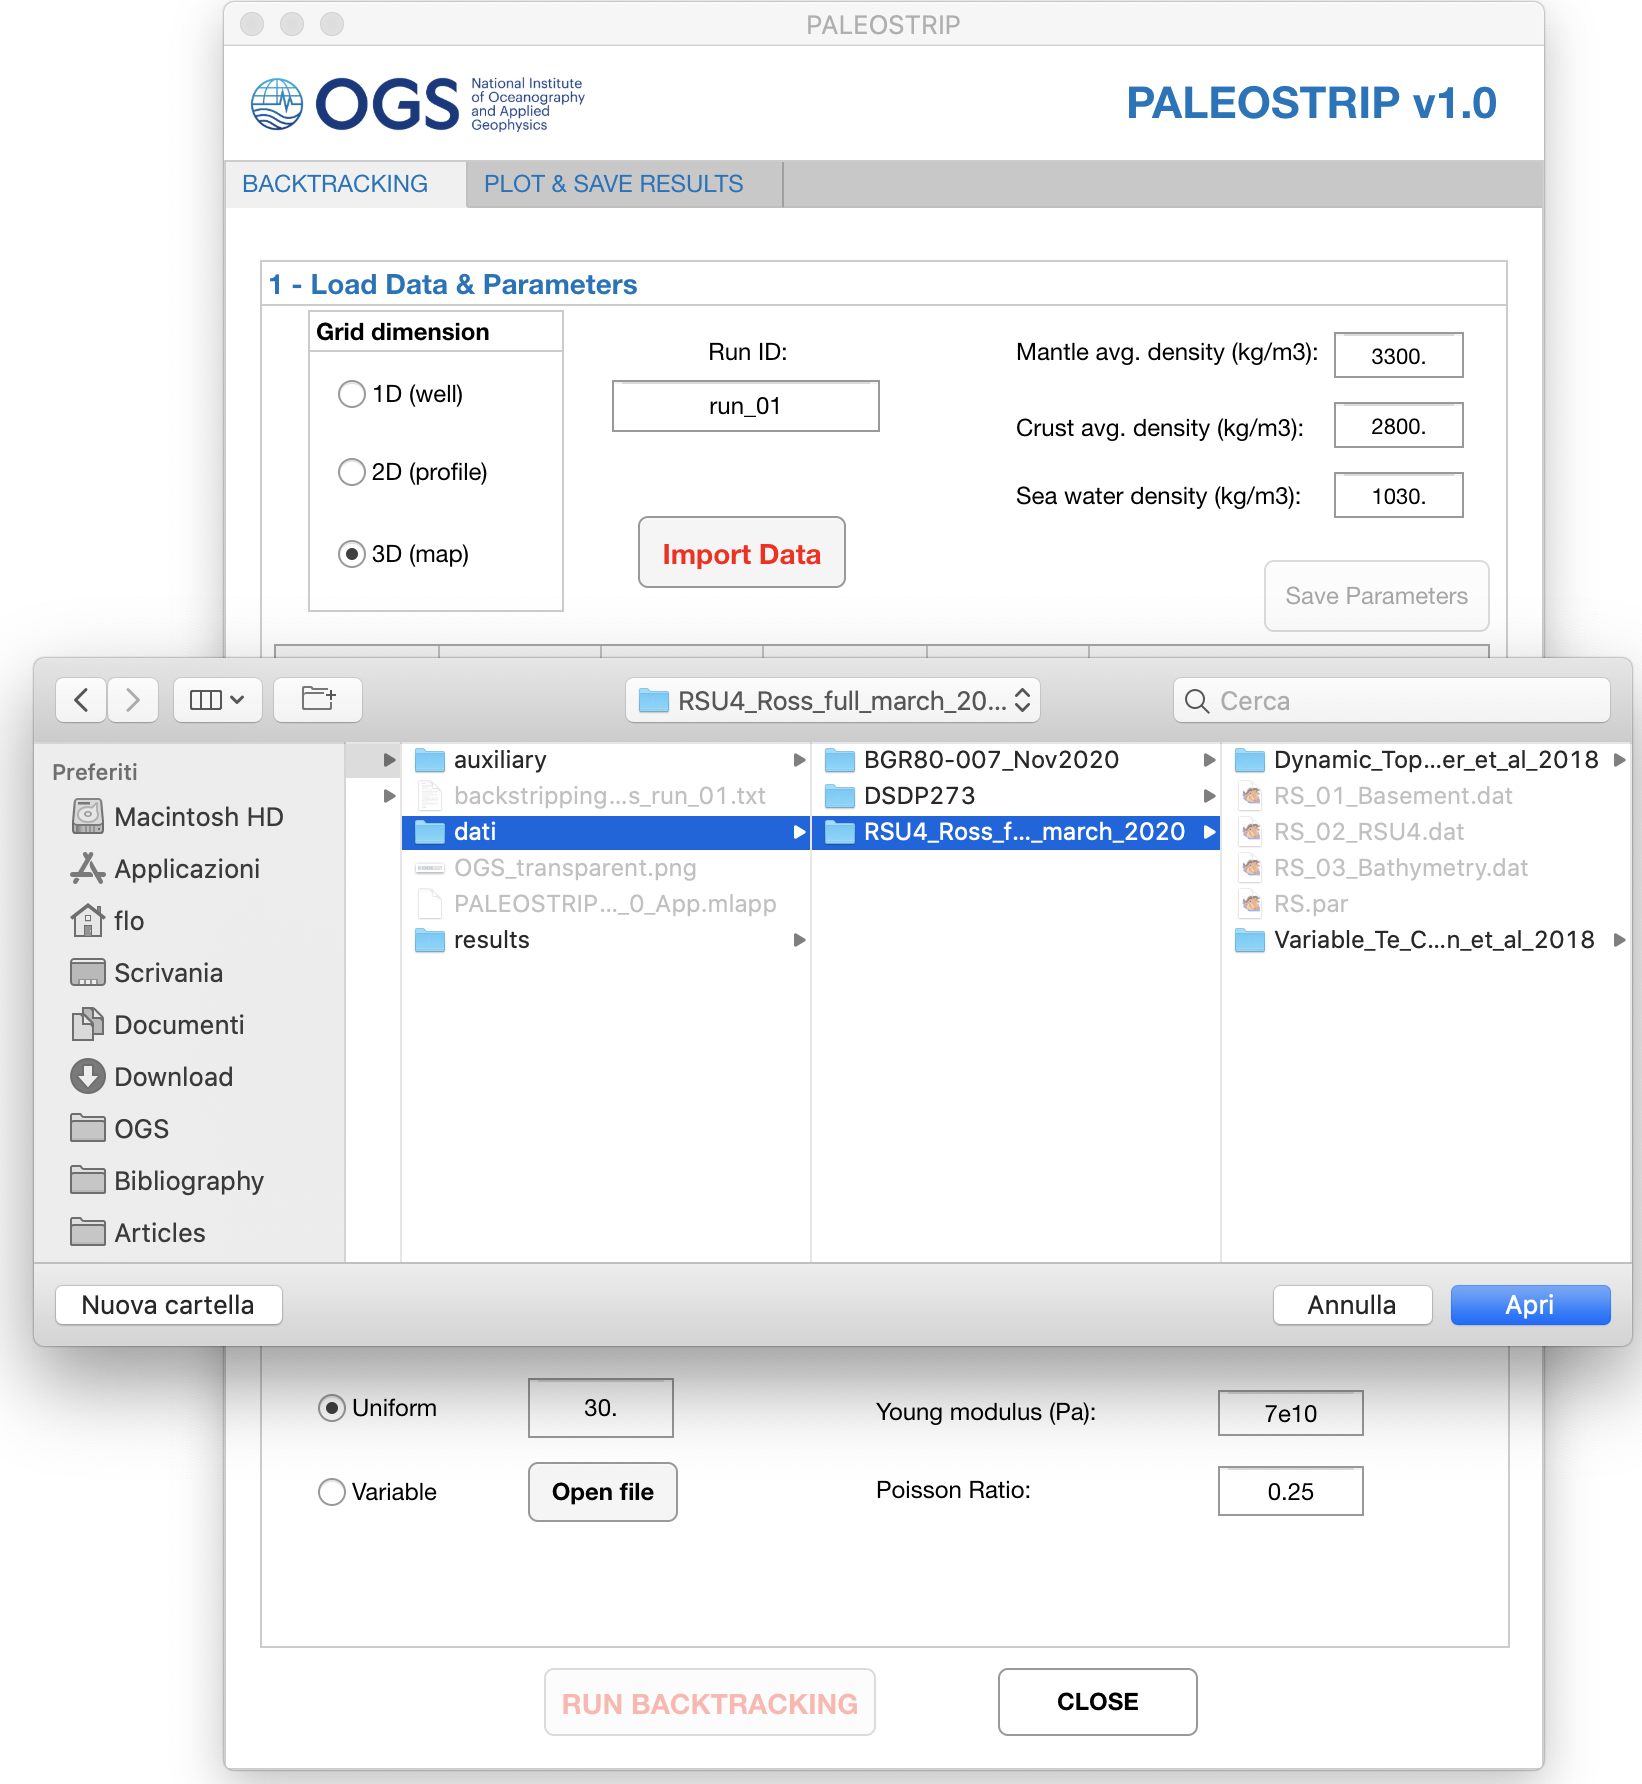
\includegraphics[scale=0.35]{Figures/3D/Import_data_3D.png}
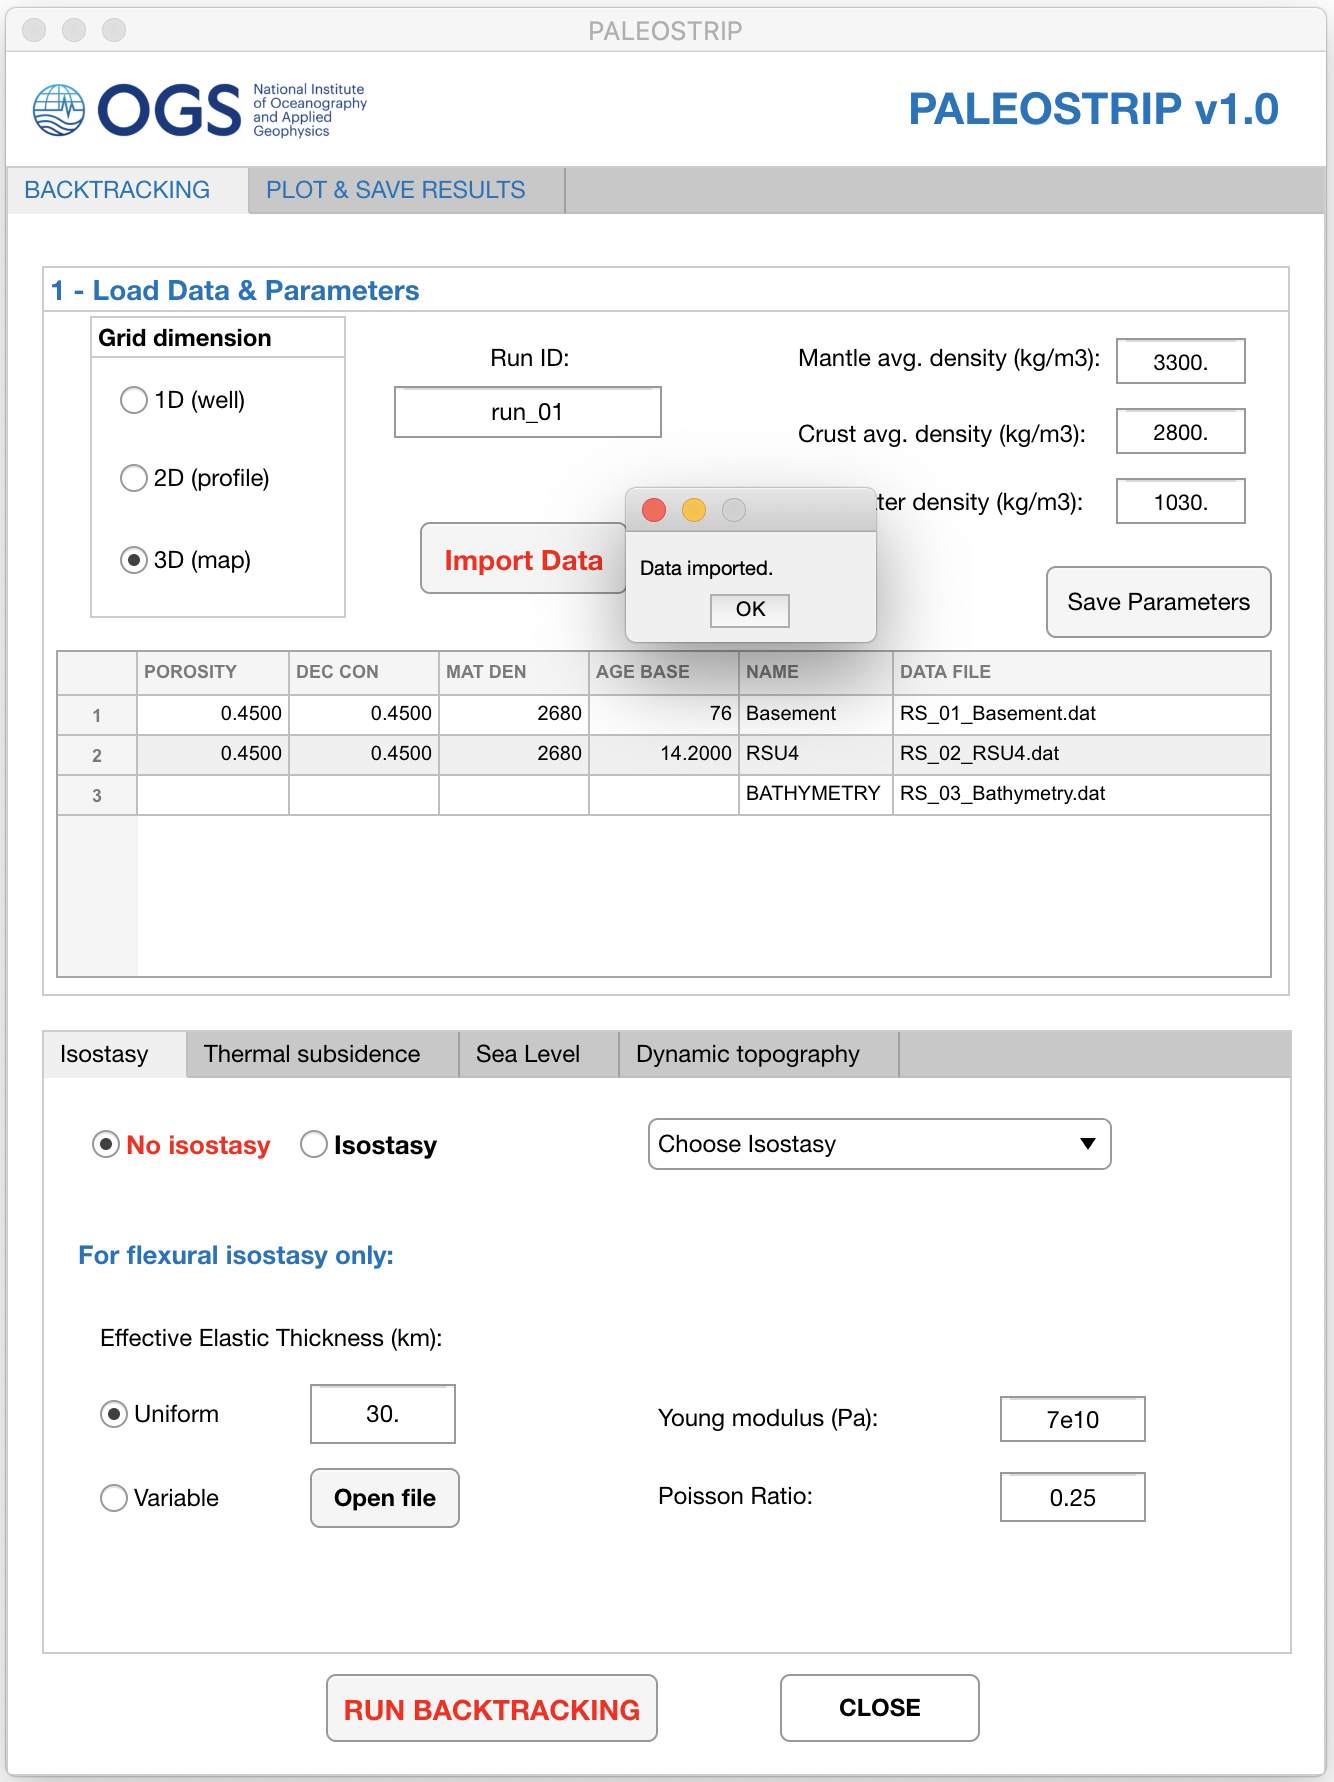
\includegraphics[scale=0.35]{Figures/3D/Import_data_OK.png}
\end{figure}

\clearpage
\newpage
\subsection*{2- Select physical parameters and corrections}

We use flexural isostasy with prescribed spatially variable effective elastic thickness from Chen et al. (2018). We also use prescribed time-evolving dynamic topography from M\"uller et al. (2018) (data files listed within a single ASCII file and passed to the GUI).

\begin{figure}[!h]
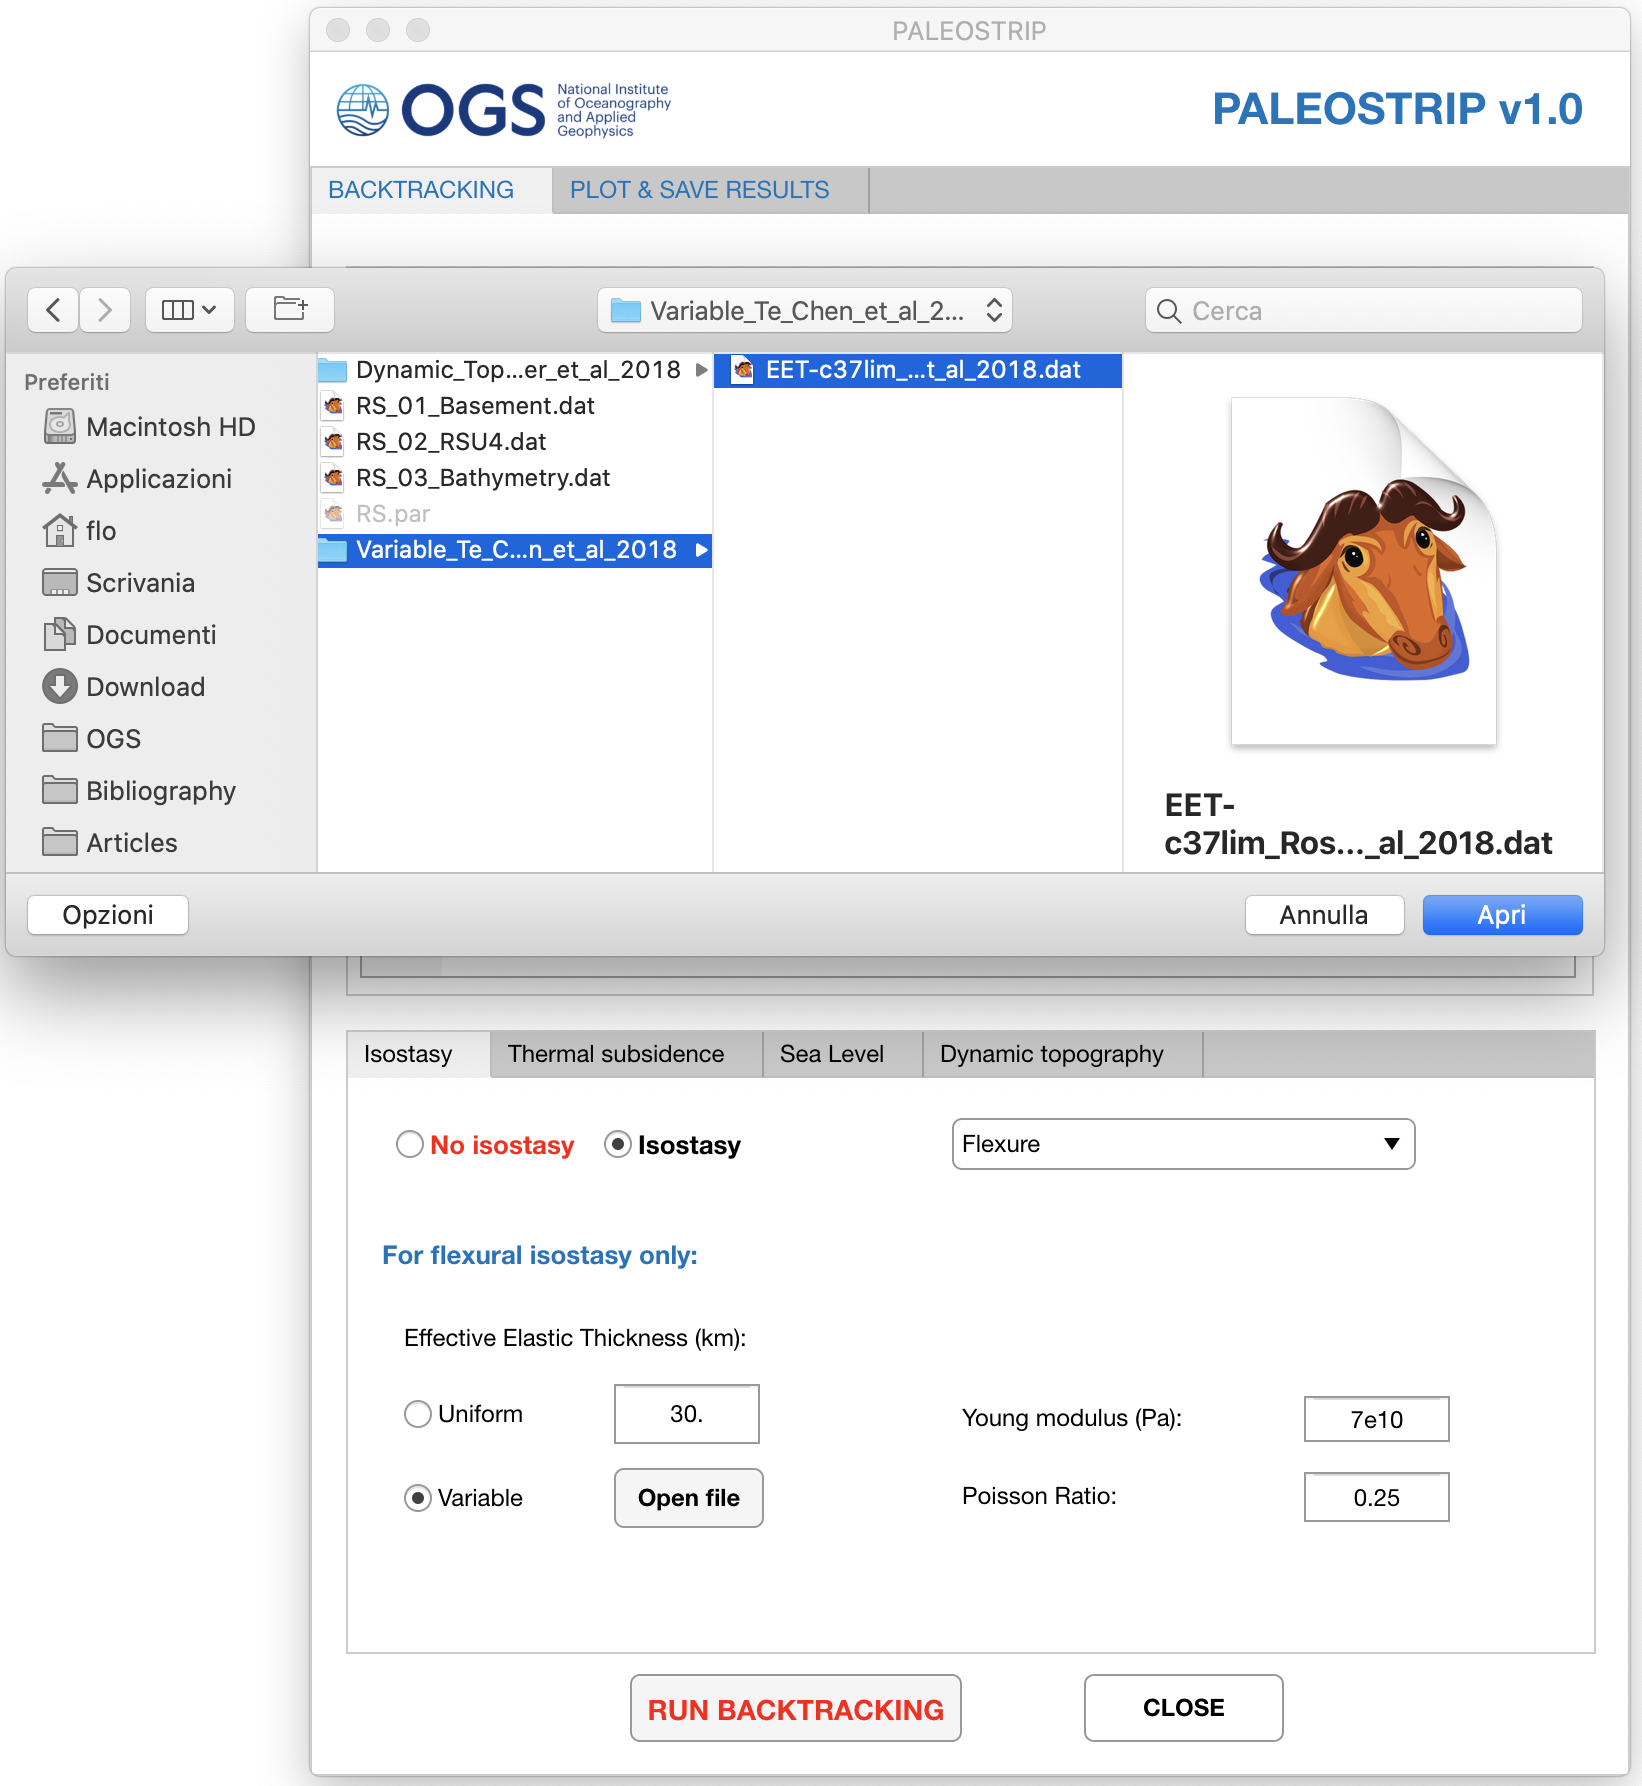
\includegraphics[scale=0.35]{Figures/3D/Variable_Te.png}
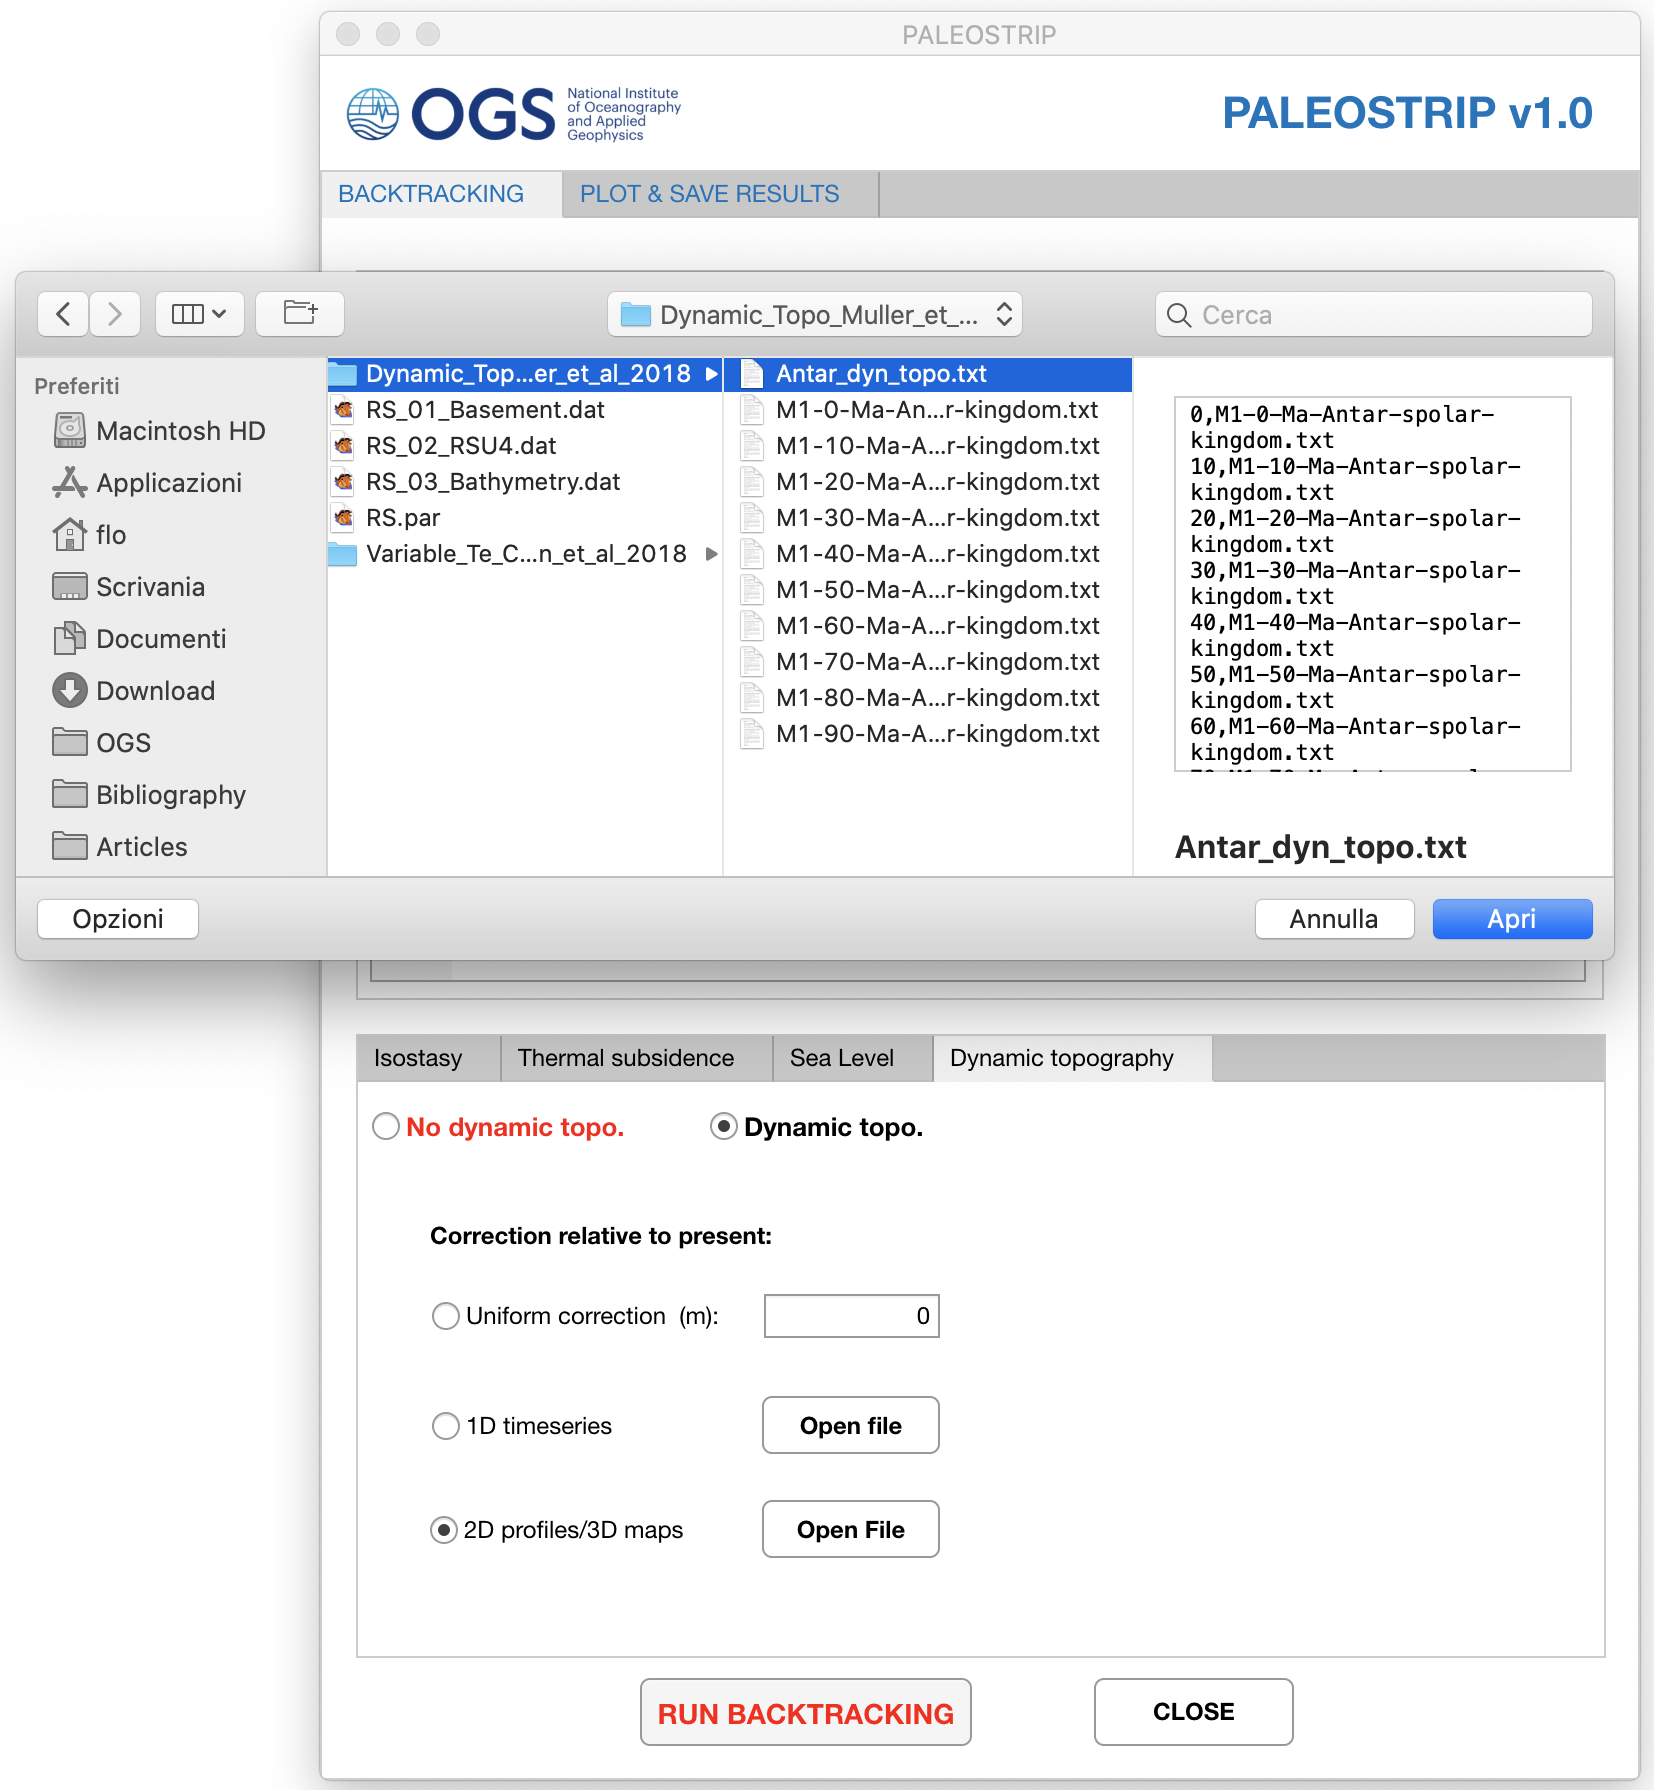
\includegraphics[scale=0.35]{Figures/3D/Dynamic_topography_Miller.png}
\end{figure}

\subsection*{3- Run Backtracking}

The procedure is identical to that shown for 1D well example above.

\clearpage
\newpage
\subsection*{4- Plot outputs}

In the case of 3D maps, several visualisation options are available. \textbf{Note that in the case of 3D maps, the plots only show the uppermost layer at each backtracking step}.\\

First we show the backtracked horizon depths with the plain map view, with a colorscale ranging from -4000 meters to +200 meters.

\begin{figure}[!h]
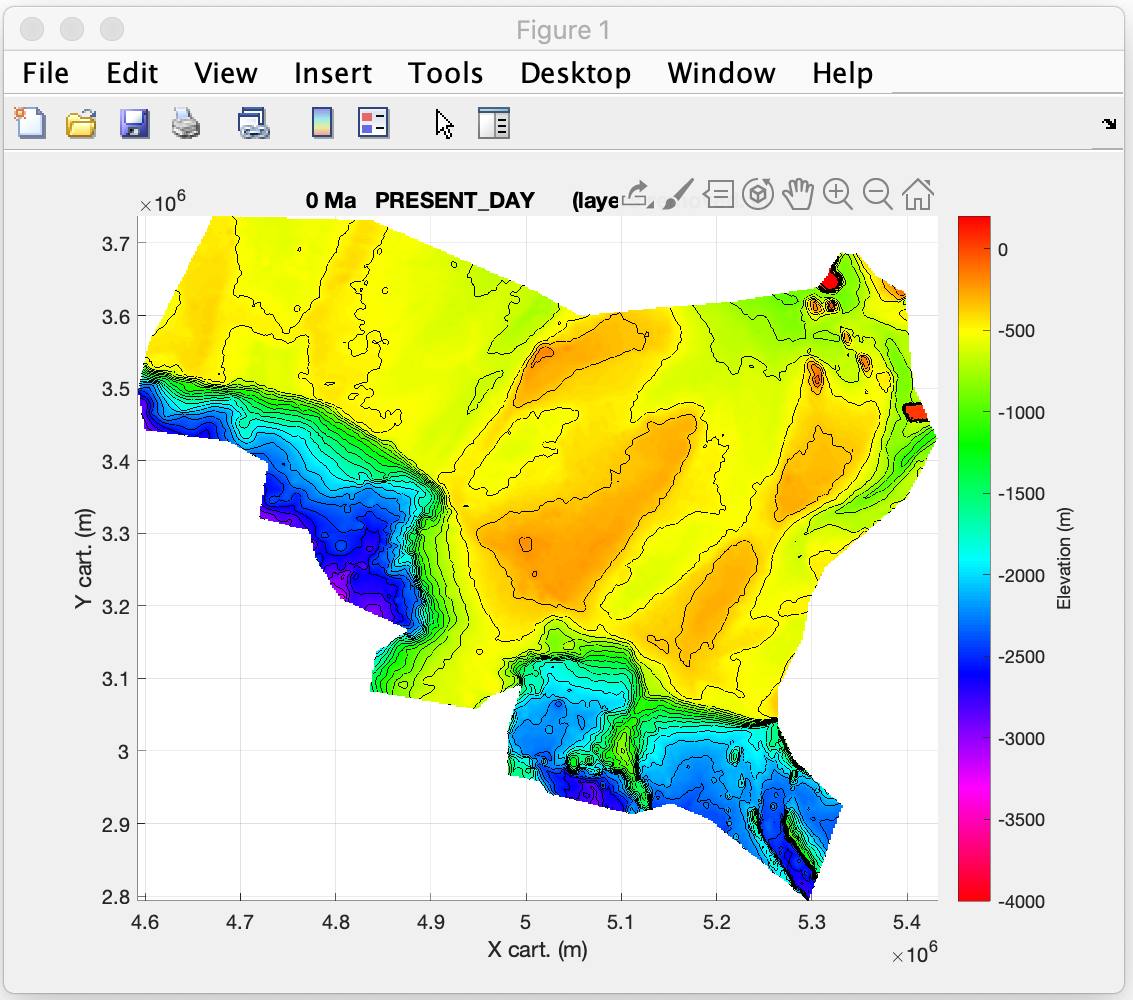
\includegraphics[scale=0.4]{Figures/3D/H03.png}\\
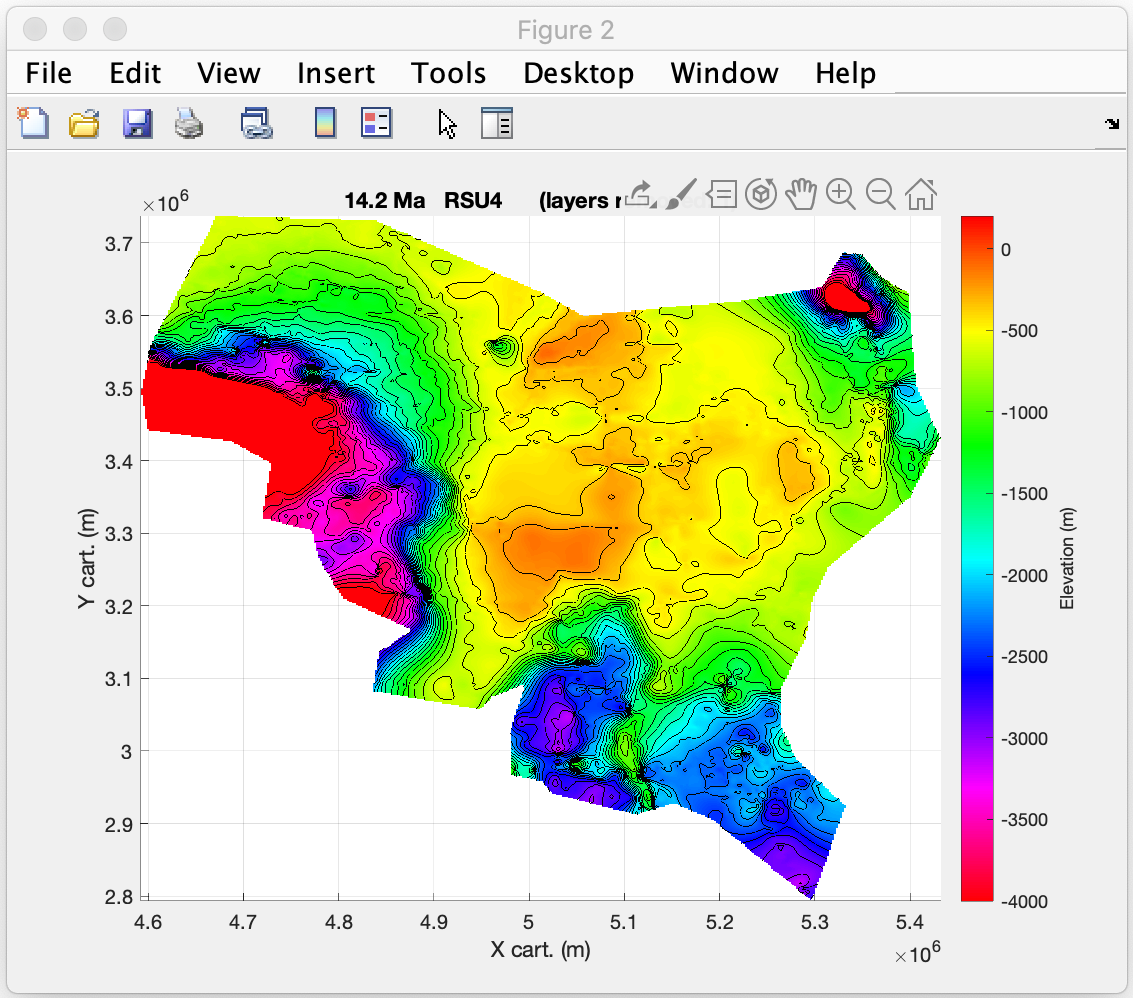
\includegraphics[scale=0.4]{Figures/3D/H02.png}\\
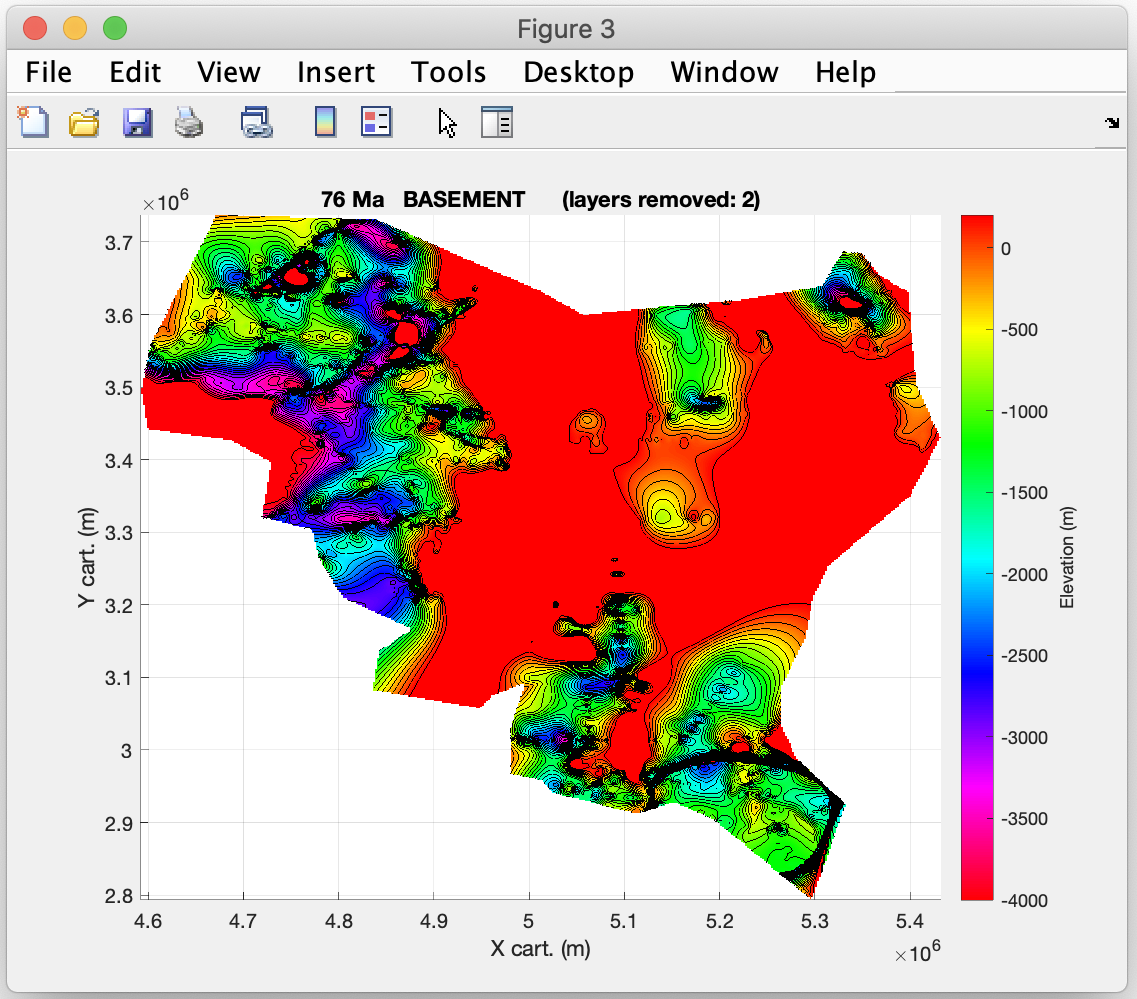
\includegraphics[scale=0.4]{Figures/3D/H01.png}
\end{figure}

\clearpage
\newpage
Then we show the same plots but with a 3D visualisation effect (\texttt{3D maps}):

\begin{figure}[!h]
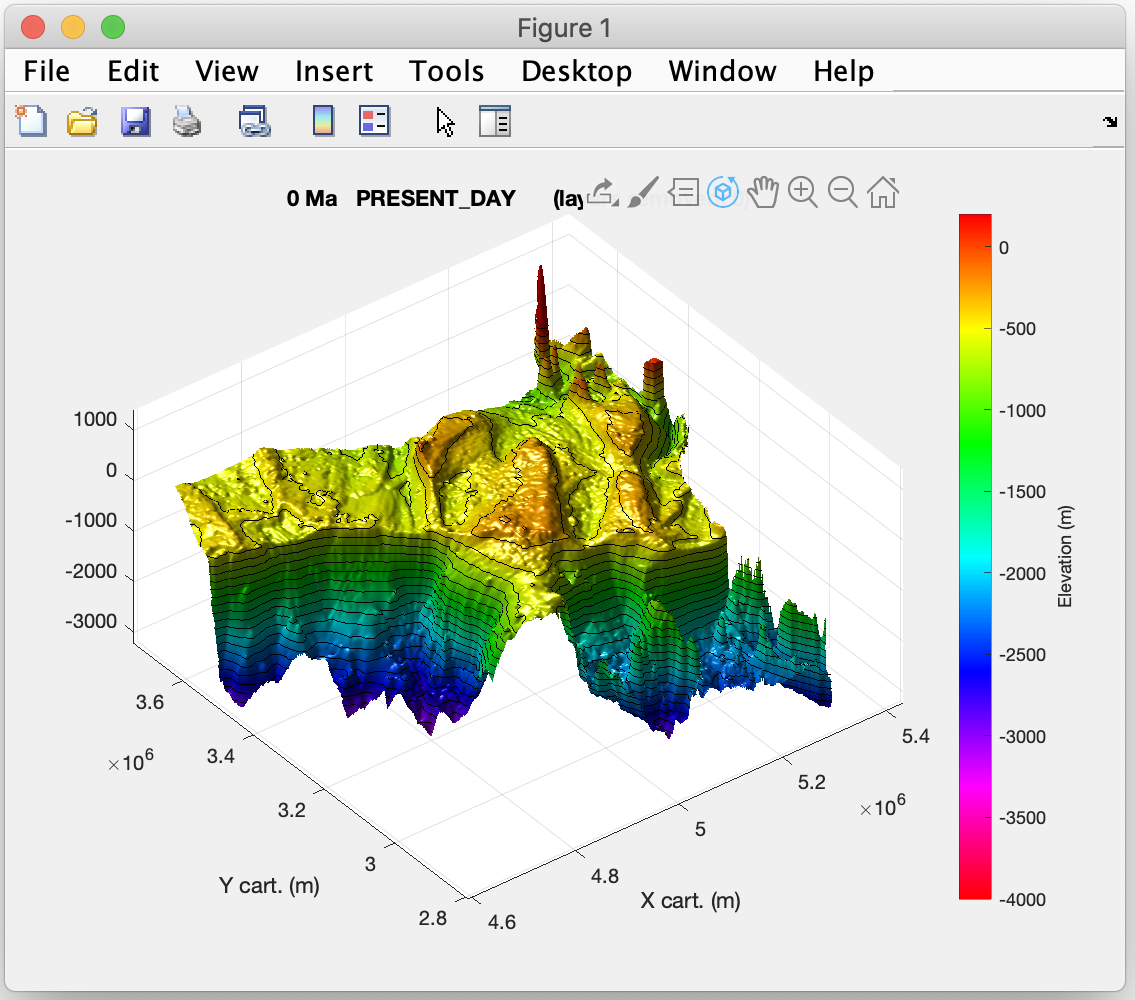
\includegraphics[scale=0.4]{Figures/3D/H03_3d.png}\\
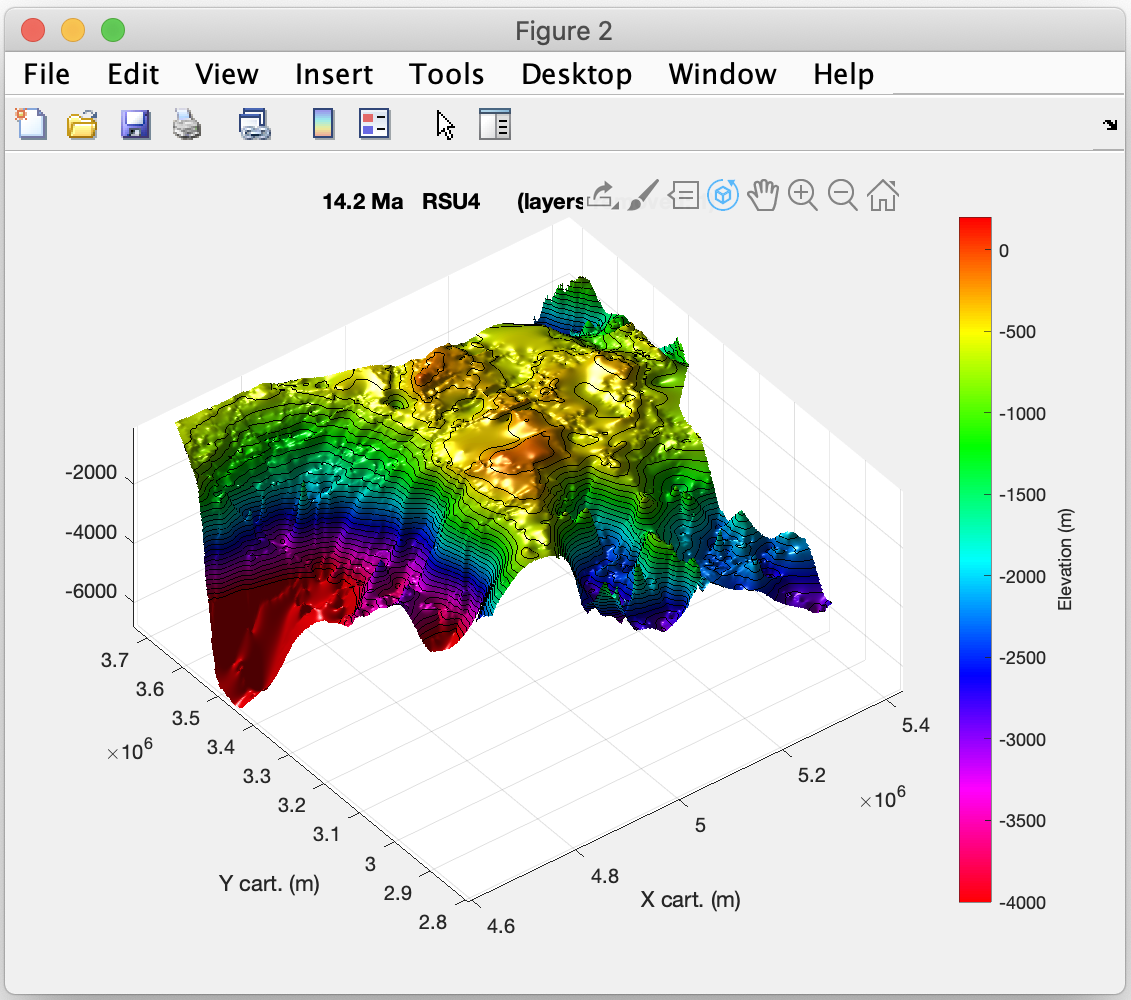
\includegraphics[scale=0.4]{Figures/3D/H02_3d.png}\\
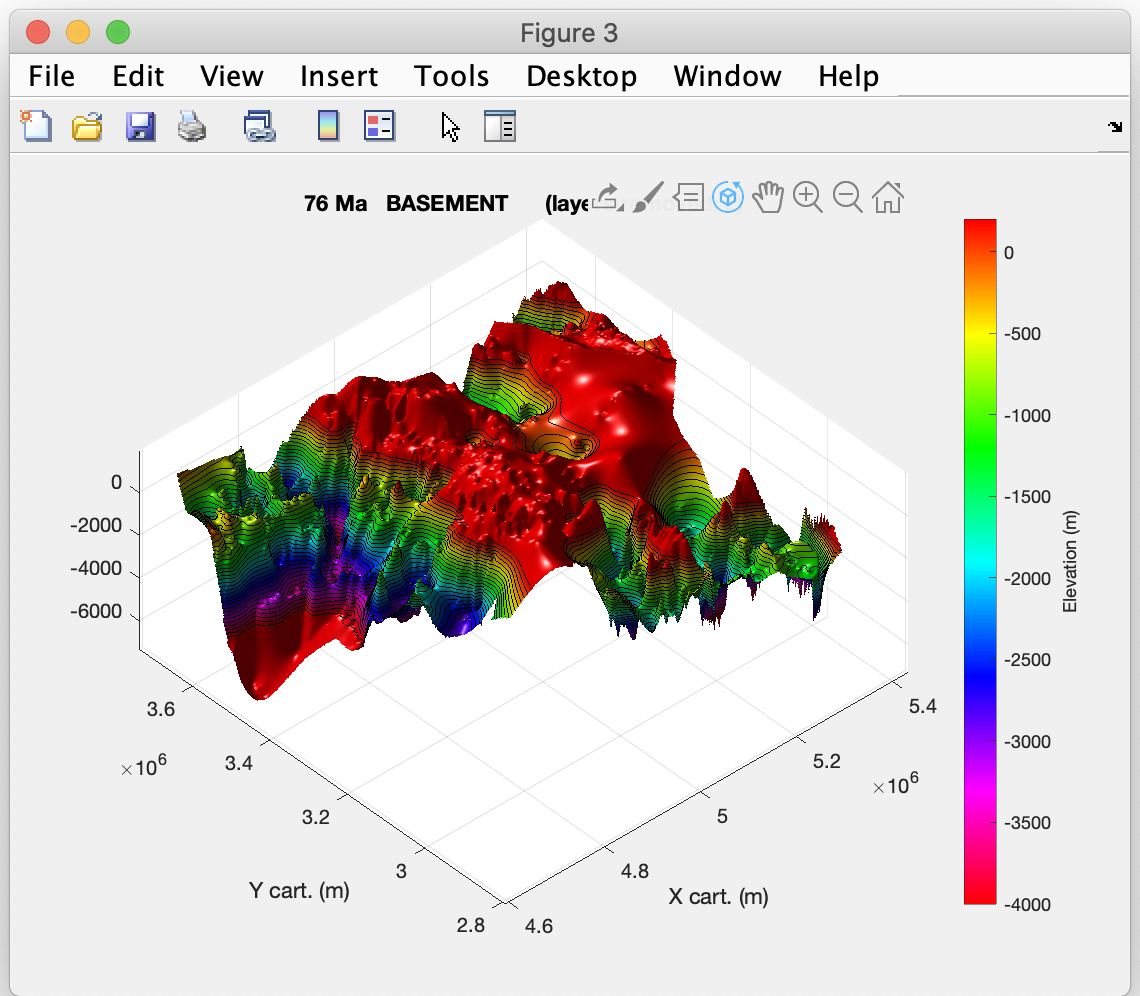
\includegraphics[scale=0.4]{Figures/3D/H01_3d.png}
\end{figure}


\clearpage
\newpage
And finally we show the same plots but with only contours displayed (\texttt{Contour (maps)} option):

\begin{figure}[!h]
\includegraphics[scale=0.4]{Figures/3D/H03_C.png}\\
\includegraphics[scale=0.4]{Figures/3D/H02_C.png}\\
\includegraphics[scale=0.4]{Figures/3D/H01_C.png}
\end{figure}


\clearpage
\newpage
\subsection*{5- Save outputs}

The procedure is identical to that shown for 1D well example above.

\subsection*{6- Extract data}

The user can extract 1d wells or 2D transects from 3D backtracked maps. Here we loaded the (X,Y) coordinates from an ASCII file to extract the data by clicking on \texttt{Load profile}. The user can also only prescribed in the Table on the GUI a starting and an ending point of a linear profile that will be created automatically by PALEOSTRIP.

\begin{figure}[!h]
\includegraphics[scale=0.4]{Figures/3D/Import_coordinates.png}
\end{figure}

The user can then select the variable to be extracted from the drop-menu and then click on \texttt{Extract}:

\begin{figure}[!h]
\includegraphics[scale=0.4]{Figures/3D/Select_variable_extract.png}\\\\
\includegraphics[scale=0.4]{Figures/3D/Extraction_OK.png}
\end{figure}

\clearpage
\newpage

\subsection*{7- Plot extracted data}

Extracted data can be plotted:

\begin{figure}[!h]
\includegraphics[scale=0.4]{Figures/3D/H03_extracted.png}\\
\includegraphics[scale=0.4]{Figures/3D/H02_extracted.png}\\
\includegraphics[scale=0.4]{Figures/3D/H01_extracted.png}
\end{figure}

\subsection*{8- Save extracted data}

The procedure is identical to that shown for 1D well example above, for saving backtracked output data.


%-----------------------------------------------------------
%BIBLIOGRAPHY
%-----------------------------------------------------------
\clearpage
\newpage

\chapter*{Bibliography}

\noindent Allen, P. A. and Allen, J. R.: Basin Analysis: Principles and Applications, 2nd Edition | , Wiley, 2 edn., 2013.\\\\

\noindent Chen, B., Haeger, C., Kaban, M. K., and Petrunin, A. G.: Variations of the effective elastic thickness reveal tectonic fragmentation of the
Antarctic lithosphere, Tectonophysics, 746, 412–424, 2018.\\\\

\noindent Colleoni, F., De Santis, L., Pochini, E., Forlin, E., Geletti, R., Brancatelli, G., Tesauro, M., Busetti, M., and Braitenberg, C., PALEOSTRIPv1.0 - a user-friendly 3D backtracking software to reconstruct paleo-bathymetries, Geoscientific Model Developments, 2021, https://doi.org/10.5194/gmd-2021-78.\\\\

\noindent Crameri, F., G.E. Shephard, and P.J. Heron (2020), The misuse of colour in science communication, Nature Communications, 11, 5444. doi:10.1038/s41467-020-19160-7. \\\\

\noindent Müller, R., Hassan, R., Gurnis, M., Flament, N., and Williams, S. E.: Dynamic topography of passive continental margins and their hinterlands
since the Cretaceous, Gondwana Research, 53, 225–251, 2018.

%%%%%%%%%%%%%%%%%%%%%%%%%%%%%%%%%%%%%%%%%%%%%%%%%%%%%%%%
%% Sample table                                        %
%% Source: www1.maths.leeds.ac.uk/latex/TableHelp1.pdf %
%%%%%%%%%%%%%%%%%%%%%%%%%%%%%%%%%%%%%%%%%%%%%%%%%%%%%%%%
%\begin{table}[ht]
%\caption{Sample table} % title of Table
%\centering % used for centering table
%\begin{tabular}{c c c c}
%% centered columns (4 columns)
%\hline\hline %inserts double horizontal lines
%S. No. & Column\#1 & Column\#2 & Column\#3 \\ [0.5ex]
%% inserts table
%%heading
%\hline % inserts single horizontal line
%1 & 50 & 837 & 970 \\
%2 & 47 & 877 & 230 \\
%3 & 31 & 25 & 415 \\
%4 & 35 & 144 & 2356 \\
%5 & 45 & 300 & 556 \\ [1ex] % [1ex] adds vertical space
%\hline %inserts single line
%\end{tabular}
%\label{table:nonlin} % is used to refer this table in the text
%\end{table}

\end{document}